% Ejemplo del uso de la template para escribir tesis/memorias de la Universidad Diego Portales.
%
% Eviar bugs a: Adín Ramírez, adin.ramirez (at) mail.udp.cl

% Puede generar borradores si omite la opción "final" de la clase.
% \documentclass{udpthesis}
\documentclass[final]{udpthesis}

% Establecemos el sistema para uso del español
% Babel ya esta cargado dentro de updthesis
\usepackage[T1]{fontenc}%    output
\usepackage[utf8]{inputenc}% input
\usepackage{lmodern}
\usepackage{multirow, array} % para las tablas
\usepackage{float}
\usepackage{longtable}
\clubpenalty=10000
\widowpenalty=10000
% Leyendas
\usepackage[font=footnotesize,labelfont=bf,labelsep=period]{caption}

% Agregue acá otros paquetes que le sean de utilidad
% Matemáticas
\usepackage{amsmath}

% Gráficos
\usepackage{graphicx}
\graphicspath{ {imagenes/} {entrevistas/}}
\usepackage[font=footnotesize,labelformat=simple]{subfig}
% Cambiamos el formato de las leyendas: finalizan en punto, y en negrita.
\captionsetup{labelsep=period,labelfont=bf}
% Habilitamos el uso de paréntesis al citar las figuras con subfiguras dentro, e.g., Fig. 1(a)
\renewcommand\thesubfigure{(\alph{subfigure})}
\renewcommand\thesubtable{(\alph{subtable})}
\newcommand{\subfigureautorefname}{\figureautorefname}

% Código
% Para generar código fuente usar listings.sty
%\usepackage{listings}
%\usepackage{tikz}
%\lstset{
%  language=[LaTeX]TeX,
%  breaklines=true,
%  basicstyle=\tt\scriptsize,
%  keywordstyle=\color{blue},
%  identifierstyle=\color{magenta},
%  commentstyle=\color{green!40!black},
%  % frame 
%  frame=tb,
%  captionpos=t,
%  xleftmargin=1em,
%  numbersep=0.3em,
%  numbers=left,
%  framexleftmargin=1.1em,
%  framexrightmargin=0pt,
%  % additional letters for accents in spanish
%  literate=%
%    {á}{{\'{a}}}1
%    {é}{{\'{e}}}1
%    {í}{{\'{i}}}1
%    {ó}{{\'{o}}}1
%    {ú}{{\'{u}}}1
%    {ñ}{{\~{n}}}1
%    {Ñ}{{\~{N}}}1
%}
%
%\renewcommand{\lstlistingname}{Código}% Listing -> Código
%\DeclareCaptionFormat{listing}{\rule{\dimexpr\linewidth\relax}{0.4pt}\par\vskip1pt#1#2#3}
%\captionsetup[lstlisting]{format=listing,singlelinecheck=false, margin=0pt,position=bottom}

% O para generar algoritmos en pseudocódigo usar algpseudocode.sty
%\usepackage{algorithm}
%\usepackage{algpseudocode}
%\makeatletter
%\renewcommand{\ALG@name}{Algoritmo}% Algorithm -> Algoritmo
%\makeatother
%\captionsetup[algorithm]{font=footnotesize,labelsep=period}

% Referencias (este paquete ordena y comprime las referencias)
\usepackage{cite}

% Un paquete para generar texto. REMUEVA ESTE PAQUETE AL UTILIZAR ESTA PLANTILLA.
\usepackage{blindtext}


% Establecemos el tema a utilizar. 
% Debe existir el archivo udpthesisEIT.sty en su sistema TeX para poder utilizarlo.
% Por ejemplo, para utilizar el tema de magíster de la EIT deben de utilizar
% \udptheme{EIT-MS}
\udptheme{EIT}


\begin{document}
%% Inicio de la portada
\frontmatter

% Título del tema (no más de 12 palabras)
\title{Propuesta de modelo predictivo para la deserción universitaria aplicado a carreras de ingeniería}
% para precisar aún más su tema, use un subtítulo
%\subtitle{Subtítulo explicativo del tema}

% El autor(es) de la tesis
\author{Jack Elgueta}
\email{jack.elgueta@mail.udp.cl}% utilice un correo que revise después de graduado

% o una lista de autores separados con comas
%\author{Juan Bar, José Foo}
%\email{juan.bar@mail.udp.cl, jose.foo@mail.udp.cl}

% Fecha a aparecer en la tesis
\date{2016}

% Profesor guía
\professor{Juan Duarte}
% Comité
\committee{Andrea Nieto}{Demian Schkolnik}

% , Demian Schkolnik

% Dedicatoria
\dedicatory{Dedico esta tesis a mi familia, especialmente a mi padre, que de un modo u otro siempre ha dado su apoyo en mis peores momentos.}

% Agradecimientos
\acknowledgment{Agradezco a todos los profesores que de un modo u otro me han otorgado el conocimiento para la elaboración de este trabajo, especialmente a mi profesor guía Juan Duarte.}

% Abstrac en inglés
\abstract{%<- evita nueva linea en el abstract
According to statistics of the Servicio de Información de Educación Superior (SIES, 2015) of the Ministry of Education reveal that over 30 \% of young people retires in the first year Career (3 of 10). In the second year this figure rises to 43 \%. Among the 20 career with the highest desertion in the country, the first and second year are the first year, 7 career engineering a dropout percentage of 36 \%, and for the second year, 12 career of engineering with a dropout percentage on 47 \%. \\


In agreement to the problematics previously mentioned, a study based on investigations will be exposed, on factors that influence the desertion of the students the careers of engineering. In order to generate a predictive model of the desertion, based on information of students of evening and diurnal day.\\

The model building will take into account factors used in other studies that determine a student's desertion, but is mainly based on three concepts. The first, Customer Intelligence, where constructs are determined on assessment of students desertion issue, thus it is expected to reach identifying variables to generate the model. The second, Business Intelligence, with which the data provided by the institutions will be processed, finding the variables identified with Customer Intelligence. And third, Data Mining, which grant the knowledge of attrition patterns in the data.
}

% Resumen
\resumen{%<- evita nueva linea en el resumen 
%El resumen no debe contener menos de 100 palabras ni mas de 300 palabras.
Según datos estadísticos del Servicio de Información de Educación Superior (SIES, 2015) del Ministerio de Educación revelan que sobre un 30 \% de los jóvenes se retira el primer año de la carrera (3 de cada 10). Al segundo año esta cifra asciende a un 43 \%. Entre las 20 carreras con mayor deserción del país, al primer y segundo año, se encuentran al primer año, 7 carreras de ingeniería con un porcentaje de deserción sobre el 36 \%, y para el segundo año, 12 carreras de ingenierías con un porcentaje de deserción sobre el 47 \%.\\

De acuerdo a la problemática anteriormente mencionada, se expondrá un estudio basado en investigaciones, sobre factores que influyen en la deserción de los alumnos en las carreras de ingeniería. Con el fin de generar una propuesta de modelo predictivo de la deserción, basados en datos de alumnos de jornada vespertina y diurna.\\

El modelo a construir tendrá en cuenta factores utilizados en otras investigaciones que determinan deserción de un alumno, pero se basará principalmente de tres conceptos. El primero, Inteligencia del Cliente, en donde se determinarán constructos, sobre apreciación de los estudiantes del tema deserción, con ello se espera llegar a la identificación de variables para generar el modelo. El segundo, Inteligencia de Negocio, con el cual se procesarán los datos otorgados por una institucion privada, encontrando las variables identificadas con Inteligencia del Cliente. Y tercero, Minería de Datos, el cual otorgará el conocimiento de patrones de deserción en los datos.\\

}

% Generamos la portada
\makecover

% Indices y listas
\tableofcontents% tabla de contenido
\listoftables%    índice de tablas
\listoffigures%   índice de figuras
% puede agregar otras listas o índices acá de ser necesario



% Inicio del contenido
\mainmatter

% Capítulos y secciones del documento
% Aca se incluyen los archivos con el texto de los capitulos
% Incluyo el archivo cap-intro.tex
\part{Marco Teórico}
\chapter[Introducción]{Introducción}
\label{ch:intro}



\section{Antecedentes y Motivación}
\label{sec:motivacion}

En Chile el tema deserción se ha transformado en un problema que preocupa tanto para el Ministerio de Educación, instituciones de educación superior y para investigaciones, por este motivo que se han comenzado a examinar modelos y a utilizar sofisticados métodos cuantitativos para entender la deserción en el contexto de educación superior. Algunos trabajos han dado como resultado que el fenómeno deserción es multicausal \cite{acuna}, específicamente, en las características individuales de pre-ingreso, tales como el establecimiento de origen, el promedio de notas y ranking en la enseñanza media, los cuales son mejores predictores de la deserción que el puntaje PSU  \cite{larroucau}. Otros resultados indican que el tipo de establecimiento de educación media impacta en la deserción. Estudiantes provenientes de colegios particulares tienen menores tasas de deserción en los últimos años de la carrera que aquellos provenientes de la educación pública \cite{celis}. También se encontró que a mayor puntaje PSU y a mayor ingreso familiar, menores son las probabilidades de deserción \cite{diaz}. \\

La motivación de esta propuesta es apoyar con información pertinente a las carreras con alto índice de deserción, principalmente carreras de ingeniería. Con el resultado se espera dar información que ayude a ejecutar acciones de tipo preventivas de apoyo tanto al docente como al alumno.\\ 

Es importante destacar que el modelo predictivo se genera a partir de la data existente, basada en la historia de las carreras de ingeniería.\\







\section{Contexto}
\label{sec:contexto}
La tasa de retención de los estudiantes en educación superior, en especial de primer año, es uno de los indicadores más utilizados a nivel internacional para medir la eficiencia interna de las instituciones de educación, considerando que la mayor parte de los estudiantes desertan al primer año. Por otro lado, la deserción, permanencia y titulación de los estudiantes universitarios se ha transformado en un elemento estratégico para las instituciones en la rendición de cuentas y también para el Ministerio de Educación, al integrar indicadores de eficiencia docente, como la tasa de retención y de titulación, con el fin de medir el uso de recursos del crédito con aval del estado, el cual está destinado al financiamiento estudiantil a partir del año 2006 este distribuye utilizando un modelo que fija un arancel de referencia para cada carrera de las universidades pertenecientes al Consejo de Rectores de Universidades Chilenas (CRUCH).\\


De acuerdo con el portal mifuturo.cl del Ministerio de Educación (diciembre, 2015), actualmente existen 157 instituciones reconocidas por el Ministerio de Educación, entre ellas 54 Centros de Formación Técnica (CFT), 43 Institutos Profesionales (IP), 25 Universidades Públicas y 35 Universidades Privadas \cite{instituciones}.\\

En un estudio del SIES del Ministerio de Educación (2014) \cite{Sies2014}, sobre retención señala que:

\begin{itemize}
    \item Las universidades tienen mayor tasa de retención que los Institutos Profesionales (IP) y los Centros de Formación Técnica (CFT). Alcanzando un 76,6 \% para Universidades, 66,6 \% para IP y 64,5 \% para CFT.
    
    \item Las carreras profesionales (con y sin licenciatura) tienen tasas de retención significativamente mayores que las carreras técnicas. Con un 75 \% para las carreras profesionales y un 65,1 \% para carreras técnicas.
    
    \item Las instituciones de educación superior acreditadas tienen persistentemente mayor tasa de retención de primer año que aquellas instituciones que no lo están. Las instituciones acreditadas tuvieron una tasa de 72,2 \%, mientras que las sin acreditación un 53,7 \%.
    
\end{itemize}

\section{Metodología de la solución}
\label{sec:descripcion}

Proponer un modelo predictivo que permita identificar los alumnos de carreras de ingeniería con una mayor probabilidad de deserción temprana, de modo que la institución pueda generar mecanismos de apoyo.\\

La solución se basa en el trabajo de un conjunto de datos de carreras de jornada vespertina y diurna de una facultad de ingeniería.\\

Con estos datos, se realizará un proceso de investigación utilizando inteligencia del cliente obteniendo variables para un tablou con el que se busca aplicar técnicas de minería de datos con el fin de determinar la influencia de los datos en el análisis predictivo.\\

Con la información otorgada a través de la investigación y prueba de diferentes modelos, se espera generar una propuesta de modelo predictivo propio. \\


\section{Objetivos}
\label{sec:objetivos}

\subsection{Objetivo general}

Proponer un modelo predictivo para detectar de forma oportuna a alumnos con mayor probabilidad de desertar de la carrera de ingeniería a través de inteligencia del cliente y minería de datos.

\subsection{Objetivos específicos}

\begin{enumerate}
\item Describir conceptos básicos de inteligencia del cliente, inteligencia de negocio y minería de datos.
\item Identificar los diferentes factores que afectan la permanencia del estudiante en su carrera académica a través de inteligencia del cliente.
\item Identificar y clasificar técnicas de minería de datos.
\item Usar minería de datos para buscar patrones que predigan el comportamiento de deserción.
\item Desarrollar diferentes modelos que determinen patrones de deserción.
\item Analizar y validar los modelos desarrollados.

\end{enumerate}

\section{Metodología de trabajo}

El trabajo será dividido en tres fases:

\begin{itemize}
    \item Fase I
    
   En esta fase se trabajará principalmente en la definición y contextualización del problema, analizando el ámbito de la deserción de manera global y a nivel país, este último separado en instituciones estatales e instituciones privadas. Se definirán conceptos básicos de inteligencia del cliente, inteligencia de negocio y de minería de datos, de manera general, para poder analizar las diferentes técnicas de minería de datos. \\
    
    Se espera para esta fase tener conocimientos fuertes del tema deserción, minería de datos, inteligencia del cliente e inteligencia de negocio para dar paso a la siguiente fase.\\
    
    \item Fase II
    
    Se trabajará en entrevistas, aplicando el concepto de inteligencia del cliente para determinar constructos que permitan identificar y determinar variables influyentes en la deserción universitaria.\\   
    
    Se espera para esta fase, definir los principales datos que influyen en la predicción de deserción.\\
    
    \item Fase III
    
    En esta fase se trabajará en la solución, generando diferentes modelos predictivos a través de la herramienta \textit{RapidMiner}, software que permite aplicar varias técnicas de minería de datos. Los modelos se generarán teniendo en cuenta las investigaciones y conclusiones de las fases anteriores. Aplicando fases del proceso de minería de datos y validando los modelos con el conjunto de datos.\\
    
    Se espera a partir de los modelos generados, realizar un análisis para determinar el modelo que mejor se adapte a la situación deserción.\\
    


\end{itemize}


%\blindtext[2]
% Incluyo el archivo cap-tema.tex
\chapter[Deserción en Chile]{Deserción en Chile}
\label{ch:tema}


\section{Deserción en Chile}
\label{sec:deserción}

En los últimos 30 años en Chile ha existido un crecimiento de manera significativo en el número de matrículas de pregrado para la educación superior, de 165 mil estudiantes matriculados a principios de los ochenta, a más de un millón de estudiantes para el año 2012.\\

El cual ha marcado un gran cambio en el sistema de educación superior, pasó de ser un sistema de élite a uno masivo. Sin embargo, este cambio trajo consigo el aumento de diferentes problemas, como es el caso de la deserción.\\

La deserción no es un fenómeno aislado, las cifras en porcentaje son muy elevadas, aproximadamente un 50 \% de los alumnos que entran a universidades o centros de formación técnica no terminan su programa de estudio al cual se matricularon, situación que preocupa tanto al Estado como a los distintos actores del sistema. El Estado pierde recursos, los estudiantes y sus familias pierden la inversión en la formación de quienes no completan sus estudios, las instituciones se ven afectadas ya que dejan de recibir recursos asociados a estos estudiantes y deben adaptar su funcionamiento en cursos superiores a un menor número de alumnos. Además, para los jóvenes que desertan sus sueños de graduarse se estancan, lo que les genera frustración y descontento.\\


\subsection{Estadísticas de deserción en Chile}

En Chile desde el año 2006 surge el Servicio de Información de Educación Superior (SIES), del Ministerio de Educación, a través del mandato establecido en la Ley 20.129, la que en su artículo 49 \textsuperscript{\underline{o}} señala ``corresponderá al Ministerio de Educación, a través de su División de Educación Superior, desarrollar y mantener un Sistema Nacional de Información de la Educación Superior, que contenga antecedentes necesarios para la adecuada aplicación de las políticas públicas destinadas al sector de educación superior, para la gestión institucional y la información pública de manera de lograr una amplia y completa transparencia académica, administrativa y contable de las instituciones de educación superior'' \cite{sies}. \\

El SIES recopila datos de las matriculas de prácticamente la totalidad de las instituciones de educación superior, con los cuales genera informes anuales de las tasas de retención. La retención se es la contraparte de la deserción, indica cuántos alumnos siguen sus estudios y logran continuar a la obtención de su título. El documento más reciente sobre las tasas de retención de las instituciones abarca los años 2010 al 2014 y se puede ubicar en \cite{Sies2014}. Dicho documento, operacionalmente, calcula la tasa de retención al primer año como el cociente entre el número de estudiantes que ingresan como alumnos de primer año a un programa de estudios en un año determinado y el número de estos mismos estudiantes que se mantienen como estudiantes antiguos en la misma institución al año siguiente.\\

A continuación, se presentará una serie de estadísticas que describen el comportamiento de la retención entre los años 2010 y el año 2014.\\

\begin{figure}[H]
	\centering 
	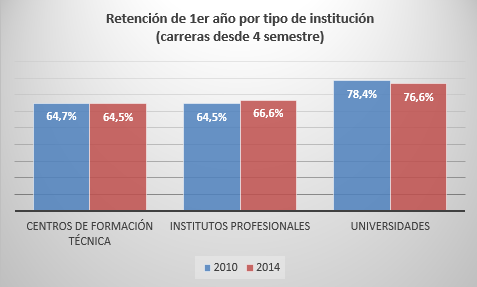
\includegraphics[width=10cm,height=5cm] {retencioninstituciones.png} 
	\caption{Retención de 1er año por Tipo de Institución} \label{fig:institucion}
\end{figure}

En la Figura \ref{fig:institucion} se puede apreciar la evolución de la retención en las instituciones chilenas entre los años 2010 y 2014. En el año 2014 la retención, tanto el CFT como en Universidades bajó con respecto al año 2010, la disminución se distribuye en un 0,2 \% para CFT, y de un 1,8 \% para Universidades, mientras que los Institutos registraron un alza de 2,1 \%. \\

\begin{figure}[h]
	\centering 
	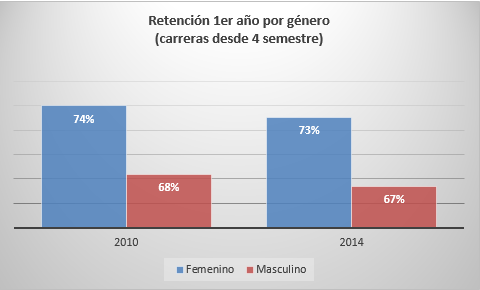
\includegraphics[width=10cm,height=5cm] {retenciongenero.png} 
	\caption{Retención de 1er año por Género} \label{fig:genero}
\end{figure}


En cuanto a género la evolución de la tasa de deserción se puede apreciar en la Figura \ref{fig:genero}, donde para ambos género ha existido una baja en la tasa de retención, para el año 2010 se registra un 74 \% para el género femenino y un 68 \% para el género masculino, y para el año 2014 se registra un 73 \% para el género femenino, y un 67 \% para el género masculino, ambos con una baja de 1 \%.\\  

\begin{figure}[H]
	\centering 
	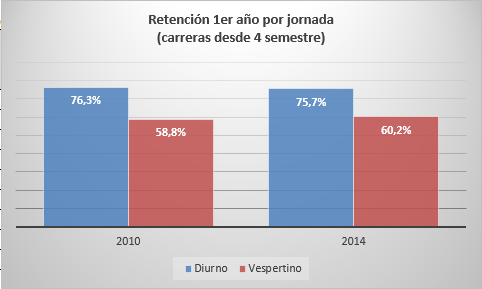
\includegraphics[width=10cm,height=5cm] {retencionjornada.png} 
	\caption{Retención de 1er año por Jornada} \label{fig:jornada}
\end{figure}

En lo que respecta a las jornadas de estudios, para el año 2010 la tasa de retención para carreras diurnas fue del 76,3 \% y para carreras vespertinas fue de un 58,8 \%, mientras que para el año 2014, para la jornada diurna fue de 75,7 \% teniendo una baja de 0.6 \%, y para la jornada vespertina, fue de 60,2 \% obteniendo un incremento de 1,4 \%, ver Figura \ref{fig:jornada}.\\

\begin{figure}[h]
	\centering 
	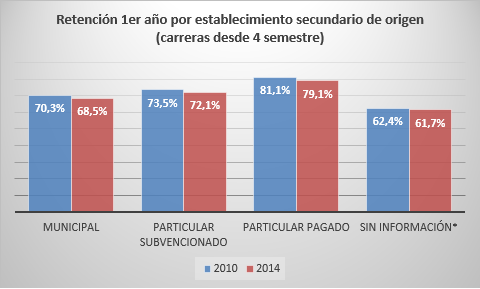
\includegraphics[width=10cm,height=5cm] {retencionestablecimiento.png} 
	\caption{Retención de 1er año por Establecimiento de Origen} \label{fig:establecimiento}
\end{figure}


La Figura \ref{fig:establecimiento}, genera la estadística a partir de los establecimientos de origen de los alumnos, mostrando para el año 2010 los siguientes resultados. Para establecimientos municipales un 70,3 \%, para establecimientos particular subvencionado un 73,5 \%, para establecimientos particular pagado un 81,1 \% y para establecimientos sin información (matricula sin información de colegio de origen) un 62,4 \%. Para el año 2014, para establecimientos municipales hubo una baja de 1,8 \%, marcando 68,5 \%, para establecimientos particular subvencionado hubo una baja de 1,4 \%, marcando 72.1 \%, para establecimientos particular pagado hubo una baja de 2 \%, marcando 79.1 \%, para establecimientos sin información, también hubo una baja de 0,7 \%, marcando 61.7 \%.  \\

\begin{figure}[h]
	\centering 
	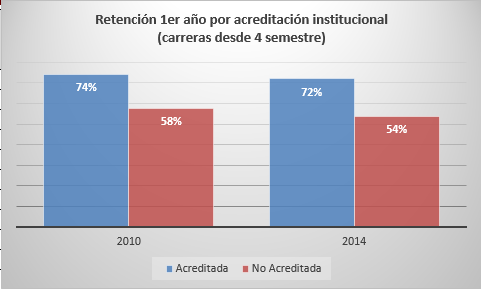
\includegraphics[width=10cm,height=5cm] {retencionacreditacion.png}
	\caption{Retención de 1er año por Acreditación Institucional} \label{fig:acreditacion}
\end{figure}

La estadística para instituciones con y sin acreditación se puede visualizar en la Figura \ref{fig:acreditacion}. La retención el 2010, para instituciones acreditadas fue de 74 \% y para instituciones no acreditadas de 58 \%. Para el año 2014, las instituciones acreditadas bajaron 2 \%, alcanzando un 72 \%, mientras que las no acreditadas llegaron al 54 \%, registrando una baja de cuatro puntos porcentuales.\\   


% incluya otros archivos según su necesidad
% \input{archivo}
\chapter[Inteligencia del Cliente]{Inteligencia del Cliente}
\label{ch:ic}

\section{Inteligencia del Cliente}
\subsection{¿Qué es Inteligencia del Cliente?}

El proceso de Inteligencia del Cliente (Customer Intelligence, CI), gestiona, almacena y analiza datos e información relacionada a los clientes, buscando un mayor entendimiento de sus necesidades, para así mejorar el flujo de comunicación, el servicio prestado y diseñar y/o preparar decisiones estratégicas concretas.\cite{ic}\\

En otras palabras, consiste en convertir los datos en bruto con los que se cuentan, en información científica útil y analizable. \cite{ic}\\

Una gestión adecuada de CI, trae consigo beneficios para la empresa u organización. Mejorando la experiencia del servicio al cliente, toma estratégica de decisiones y predicción de hábitos o comportamiento del cliente.\cite{ic}\\

Inteligencia del Cliente está fuertemente relacionado a la ``Gestión de Relación con el Cliente'' (Customer Relationship Management, CRM), CI es un componente clave para CRM, ya que CI capta datos e información del cliente que CRM no logra hacer. CI se basa en apreciaciones, opiniones del cliente, principalmente en aspectos de emociones que provoca el servicio y/o producto entregado por la empresa. En cambio, un sistema tradicional de CRM obtiene los datos e información del cliente basado en historiales, como por ejemplo historial de compras. Aplicando ambos conceptos de manera efectiva, CI otorga una importante fuente de información con respecto a comportamiento y experiencia de los clientes de una empresa.\cite{wikiic}\\



\subsection{Estructura de Relacionamiento y CRM}

Inteligencia del Cliente estudia, desde los ámbitos psicológicos y sociales al ser humano y su forma de relacionarse con el resto, ya que busca como objetivo relacionar los clientes con la empresa, tal como relacionarse con otro ser humano, generando un compromiso con una carga emocional.\\


La gestión de relación con el cliente CRM, es parte de una estrategia centrada en el cliente, una parte fundamental de su idea, es la recopilación de la mayor cantidad de información posible de los clientes, para poder entender sus necesidades y dar valor a la oferta.\cite{crm}\\


Los sistemas informáticos ayudan a gestionar la relación con el cliente, almacenando sus datos y aplicando Inteligencia de Negocio en conjunto con minería de datos.

\subsection{Metodología de la Metáfora}

La metodología de la metáfora es una herramienta del marketing que analiza el pensamiento consciente e inconsciente del consumidor, teniendo en cuenta puntos de neurociencia y psicología con el objetivo de comprender sus emociones y motivaciones, ya que están estrechamente relacionadas con los procesos del razonamiento y por ende las emociones contribuyen a una toma de decisiones sólidas.\footnote{``Viaje desde lo conocido'', Zalman Cap. 1}\\

En marketing, se piensa que el consumidor capta sus recuerdos como una cámara, un mecanismo que capta imágenes, pero con un toque de creatividad, lo que hace el recuerdo maleable, es decir, cambian constantemente de forma inconsciente, haciendo que los recuerdos sean metáforas. \\

Cuando los consumidores usan las metáforas para describir un producto o servicio llevan sus pensamientos y sentimientos inconsciente a un nivel de consciencia que permite encontrar sentido a lo que descubren e influye en sus decisiones y acciones. Esto permite a las empresas y organizaciones diseñar ofertas más valiosas para los consumidores.\footnote{``Interrogar a la mente'', Zalman Cap. 4}\\

En las ciencias cognitivas el captar o inferir el pensamiento de una persona a través de sus declaraciones o conductas es conocido como ``constructos''. Los constructos no son el pensamiento ni la conducta real de la persona, más bien es una interpretación que realiza en este caso el mercadólogo del consumidor.\footnote{``Pensándolo bien'', Zalman Cap. 6}\\

Los constructos son más bien etiquetas que realiza una persona, a partir del análisis del comportamiento de otra. Los constructos pueden tener asociaciones entre si, generando un ``mapa de consenso''. Un mapa de consenso nace a partir de los constructos de un grupo de personas, y se trata de un gráfico de pensamientos y sentimientos compartidos de un grupo sobre un tema en concreto. Figura \ref{fig:consenso}


\begin{figure}[h]
\begin{minipage}{\textwidth} 
\centering 
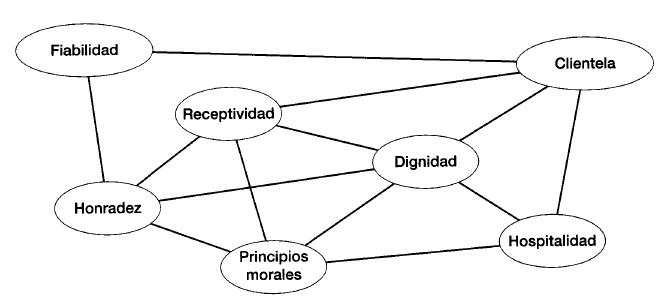
\includegraphics[width=10cm,height=5cm] {consenso.png} 
\caption[Mapa de Consenso]{Mapa de Consenso~\footnote{Fuente: Mind of the Market Laboratory/Harvard Business School}}
\label{fig:consenso}
\end{minipage}
\end{figure}

La metodología de la metáfora se aplica en entrevistas, las cuales pueden ir variando dependiendo del objetivo de la investigación, para el trabajo que se realizará en esta investigación, se seguirán los siguientes pasos:\\

\begin{enumerate}
\item Recolección de revistas o periódicos con muchas imágenes.
\item Pedir al entrevistado que recorte imágenes que se relacionen o motiven sobre un tema en concreto.
\item Pedir que describan las imágenes recortadas y luego las agrupen en distintos grupos, señalando un tema por grupo.
\item Realizar una pregunta opuesta al tema en concreto y tomar apuntes respecto a las respuestas.
\item Definir constructos a partir de las apreciaciones que se obtuvieron con las descripciones de las imágenes y respuestas de la pregunta opuesta.
\item Identificar relaciones entre los constructos definidos y crear un mapa de consenso.
\item Generar métricas y variables a partir de los constructos y sus asociaciones.

\end{enumerate}

\section{Inteligencia de Negocio}

Inteligencia de Negocio (Business intelligence, BI), es el proceso que permite transformar los datos en información y la información en conocimiento, permitiendo ayudar a la empresa u organización en la toma de decisiones.\cite{bi}\\

BI nace debido a la gran cantidad de datos que manejan las organizaciones, lo que, a través de la combinación de tecnología, herramientas y procesos, logra la transformación de datos. Dentro de las tecnologías utilizadas en las empresas, se pueden identificar dos tipos de sistemas, los sistemas OLTP que proporcionan datos de orígenes y los sistemas OLAP que ayudan a analizar dichos datos: \cite{olapvsoltp}\\


\begin{enumerate}

    \item \textbf{Sistemas OLTP (Online Transaccional Processing, Procesamiento Transaccional en Línea):}\\
Son bases de datos orientadas al procesamiento de transacciones cortas, rápidas y en línea. Una transacción genera un proceso atómico (que debe ser validado con un commit, o invalidado con un rollback), y que puede involucrar operaciones de inserción (INSERT), modificación (UPDATE) y borrado (DELETE) de datos.\\

\item \textbf{Sistemas OLAP (Online Analytical Processing, Procesamiento Analítico en Línea):}\\
Un sistema OLAP es un vector multidimensional, de N dimensiones, en el, la información se almacena en cada una de estas dimensiones, de forma ordenada y jerarquizada, lo cual ayuda a realizar un análisis rápido de su contenido. Las dimensiones de OLAP son diferentes perspectivas de análisis de información, en donde el usuario especifica diversos criterios que definen cuál y de qué forma será presentada, acumulada y ordenada la información, obteniendo resultados a una velocidad superior e la que se obtendría con un sistema de bases de datos relacional.\\

Las acciones básicas que tienen las tecnologías que implementan un sistema OLAP son: \cite{bi}

\begin{itemize}
    \item Segmentar: Agrupar datos por condiciones especificadas.\\
\item Filtrar: genera informes de datos acotados por algún parámetro.\\
\item Profundizar (Drill down): Desglose de un dato, ejemplo, el desglose de un semestre, sería el mes.\\
\item Sintetizar (Drill up): Deshace el desglose de ``Profundizar''.\\
\item Rotar (Drill anywhere): Realiza un desglose por una característica de una jerarquía distinta a la que se está visualizando actualmente.\\

    
\end{itemize}
    
\end{enumerate}

    Cada uno de estos sistemas están hechos para realizar una tarea específica, por lo cual, a pesar de que ambas son bases de datos, tienen diferencias. A continuación se detallan las principales diferencias entre los sistemas OLTP y OLAP, Tabla \ref{tabla:oltpvsolap}.

\begin{table}[H]
\centering
\begin{tabular}{|c|c|}
\hline
OLTP & OLAP\\ \hline
Son la fuente original de los datos & Los datos OLAP provienen de OLTP \\ \hline
Actualización en tiempo real &	Solo realiza procesos de carga \\ \hline
Por lo general muy rápidos & Lento debido a la gran cantidad de datos a procesar \\ \hline
Consultas simples y estandarizadas & Consultas complejas \\ \hline
Bases de datos normalizadas &	Bases de datos desnormalizadas \\ \hline
Utilizan poco espacio & Requiere una gran cantidad de espacio \\ \hline
\end{tabular}\newline
\caption{Diferencias OLTP vs OLAP. \cite{tablaolapvsoltp}}
\label{tabla:oltpvsolap}
\end{table}

Los sistemas OLTP se pueden utilizar de manera independiente de OLAP, sin embargo, cuando una empresa maneja grandes cantidades de datos, es necesario utilizar una arquitectura que involucra ambos sistemas. Arquitectura que maneja los siguientes componentes:


\begin{itemize}
    \item Bases Operacionales (OLTP).
    \item Procesos ETL
    \item Área Staging
    \item Base Analítica (Data Warehouse)
    \item Herramientas de gestión
\end{itemize}

Estos componentes son los que conforman el proceso de Inteligencia de Negocio, y se puede visualizar en el siguiente esquema, Figura \ref{fig:esquemaBI} :

\begin{figure}[H]
\begin{minipage}{\textwidth}
\centering 
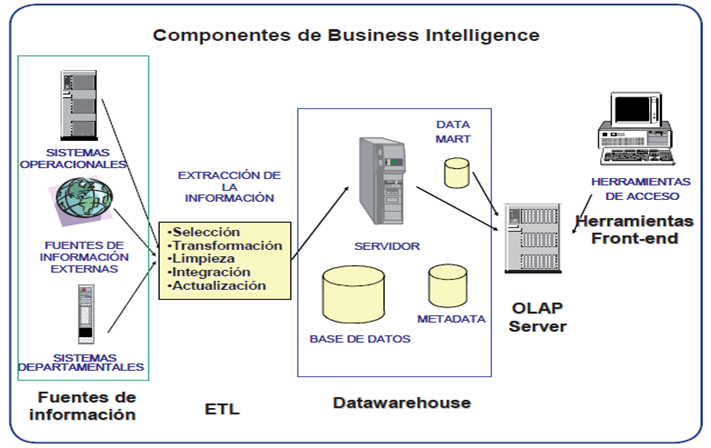
\includegraphics[width=12cm,height=7cm] {componentesBI.png}
\caption[Esquema de Inteligencia de Negocio]{Esquema de Inteligencia de Negocio~\footnote{Curso Inteligencia de Negocios 2/2015, UDP}}
\label{fig:esquemaBI}
\end{minipage}
\end{figure}

\subsection{Bases Operacionales}

Las bases operacionales son las encargadas de almacenar todos los datos de transacciones de una organización, datos que pueden ser de diferentes fuentes, por ejemplo, bases de datos Oracle, SQL Server, Excel entre otros.

\subsection{Procesos ETL}

Los procesos ETL (del inglés, Extract, Transform, Load) son una pieza fundamental de la Inteligencia de Negocio, ya que trata del proceso de mover datos de múltiples fuentes, transformar y luego cargar en otra base de datos.\\

Estos procesos consumen entre el 60 \% y 80 \% del tiempo de un proyecto de BI, y son proceso clave en la vida del proyecto.\cite{etl}\\

ETL se divide en 5 subprocesos:

\begin{enumerate}
\item Extracción:
Recupera los datos necesarios físicamente de las distintas fuentes de información, dejando los datos en bruto. Su extracción puede ser manual o utilizando una herramienta. Sus principales problemas son las distintas fuentes de datos y distintas plataformas.

\item Limpieza:
Recupera los datos en bruto y comprueba su calidad, elimina los duplicados y, cuando es posible, corrige los valores erróneos, si existen valores vacíos, los completa siempre y cuando sea posible.\\

Estos valores, generalmente se llaman valores sucios, y es muy probable encontrarlos, lo importante es saber el origen de dicha suciedad.\\

La limpieza se divide en distintas etapas:
\begin{itemize}
    \item Depurar los valores:
    Localiza elementos individuales de las fuentes de datos y los aísla en estructura de destino, por ejemplo, Dirección $\rightarrow $ calle, número, comuna, ciudad.
    
    \item Corregir:
    Corrige los datos individuales utilizando algoritmos y fuentes de datos externas.
    
    \item Estandarizar:
    Se trabaja con formatos de datos definidos y se aplican rutinas para homogeneizar datos. 
    
    \item Relacionar:
    Busca y relaciona los valores de los registros, corrigiéndolos y estandarizándolos según reglas del negocio, eliminando datos duplicados.
    
    \item Consolidar: 
    Analiza e identifica relaciones entre registros relacionados y los junta en una sola representación.

\end{itemize}

\item Transformación:
Recupera los datos limpios y de alta calidad, los estructura y suma en distintos modelos de análisis.

\item Integración:
Valida que los datos cargados son consistentes con las definiciones y formatos de la base analítica. Integra los datos en los distintos modelos de las distintas áreas de negocio que se han definido.

\item Actualización:
Se añaden los datos a la base analítica.


\end{enumerate}


\subsection{Área Staging}

El área staging es una base de datos la cual es una copia de todas las bases operacionales, generada principalmente para realizar las siguientes actividades:

\begin{itemize}
    \item Facilitar extracción de datos.
    \item Limpiar y mejorar la calidad de los datos.
    \item Operar y ejecutar procesos sin afectar el funcionamiento de las bases operacionales.
\end{itemize}

\subsection{Base Analítica (Data Warehouse)}

La base analítica o Data Warehouse es un repositorio o colección de datos orientada a un tema, integrada, variante en el tiempo y no volátil, que apoya el proceso de toma de decisiones de gestión.\\

En la base analítica se almacenan todos los datos procesados de Área Staging y ETL.\\

Un Data Warehouse puede tener varios DataMart, un DataMart son pequeños Data Warehouse que almacenan datos específicos de un área de negocio o departamento de una empresa.\\

A continuación se detallan las principales diferencias entre las bases operacionales y las bases analíticas, Tabla \ref{tabla:bdovsbda}. 

\begin{table}[H]
	\begin{minipage}{\textwidth} 
		\centering
		\begin{tabular}{ | c | c |}
			\hline
			BD Operacional & BD Analítica\\ \hline
			De transacciones & De consultas masivas \\ \hline
			Predomina la actualización & Predomina la consulta \\ \hline
			Actualizable & Carga, pero no actualiza \\ \hline
			De tipo operativo & Análisis y toma de decisiones \\ \hline
			Datos normalizados & Datos en estrella o copo de nieve \\ \hline
			Usuarios de perfiles medios o bajos & Usuarios de perfiles altos \\ \hline
			Estructura normalmente relacional & Visión multidimensional\\ \hline
		\end{tabular}\newline
		\caption[Diferencias BD Operacional vs BD Analítica.]{Diferencias BD Operacional vs BD Analítica.~\footnote{Creación propia}}
		\label{tabla:bdovsbda}
	\end{minipage}
\end{table}


Las bases analíticas están diseñados y desarrollados para realizar consultas complejas dentro de un volumen muy grande de datos, para lo cual se necesita una arquitectura para cumplir con este propósito, existen 3 arquitecturas, MOLAP (Multidimensional), ROLAP (Relacional) y HOLAP (Híbrido), la más usada es el modelo multidimensional.\\

Los modelos multidimensionales tienen 3 conceptos principales:

\begin{itemize}
    \item Unidad de Medida:
    Atributo cuantificable asociado a los hechos. Ejemplos, Volumen de las ventas, número de transacciones efectuadas, porcentaje de beneficios.
    
    \item Tabla de Hecho:
    Tabla que almacena los valores detallados para medidas, permite realizar inserciones entre las dimensiones y las medidas.
    
    \item Dimensiones:
    Son tablas que permiten la agrupación de los hechos.

\end{itemize}

Las bases multidimensionales son utilizadas con dos esquemas:

\begin{enumerate}
	\item Esquema Estrella:
	Es un esquema simple que utiliza una tabla de hecho, una o más tablas de dimensiones desnormalizadas, que están unidas con la tabla de hecho, Figura \ref{fig:estrella}.
	
	\begin{figure}[H]
		\begin{minipage}{\textwidth} 
			\centering 
			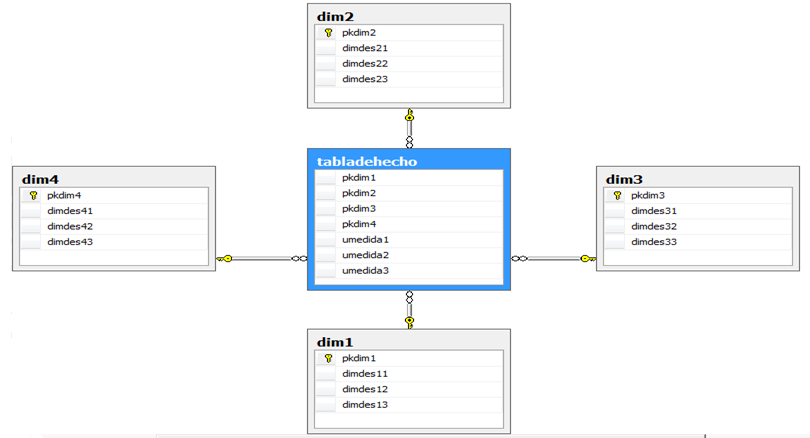
\includegraphics[width=12cm,height=7cm] {estrella.png} 
			\caption[Esquema Estrella]{Esquema Estrella~\footnote{Curso Inteligencia de Negocios 2/2015, UDP}}
			\label{fig:estrella}
		\end{minipage}
	\end{figure}
	
	\item Esquema Copo de Nieve:
	Es un esquema complejo, derivado del esquema estrella, las tablas de dimensiones se encuentran normalizadas en múltiples tablas, y la tabla de hecho no es la única que establece uniones con las otras tablas, Figura \ref{fig:copo}.
	
	\begin{figure}[h]
		\begin{minipage}{\textwidth} 
			\centering 
			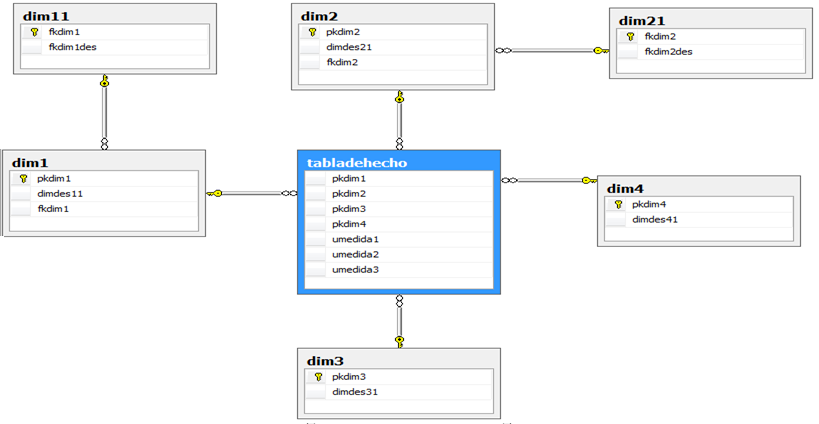
\includegraphics[width=12cm,height=7cm] {copo.png} 
			\caption[Esquema Copo de Nieve]{Esquema Copo de Nieve~\footnote{Curso Inteligencia de Negocios 2/2015, UDP}}
			\label{fig:copo}
		\end{minipage}
	\end{figure}
	
\end{enumerate}


\subsection{Herramientas de Gestión}

Después de que los datos son procesados y almacenados en la base analítica, estos se encuentran disponibles para ser visualizados y analizados a través de herramientas de gestión, que permiten a las personas de alto mando dentro de una organización tener la información de forma rápida y oportuna para la toma de decisiones. Existen una variedad de herramientas que cumplen diferentes objetivos, a continuación se identifican alguna de ellas.

\subsubsection{Query $\&$ Reporting}

Son herramientas que realizan consultas o informes que trabajan tanto sobre el detalle como sobre las agregaciones de la información. Manejan una gran cantidad de información y principalmente responden a la pregunta ¿Qué sucedió?

\subsubsection{Análisis OLAP}

Las herramientas de análisis OLAP o ``Analytics Reports'' son utilizadas por los analistas que necesitan tener la información desde distintos puntos de vistas. Estas herramientas permiten navegar dentro de la información profundizando o ir al detalle, conocidos como navegación jerárquica (Drill Down) y navegación al detalle (Drill Through). Estas herramientas responden a la pregunta ¿Por qué sucedió?

\subsubsection{Dashboard}

Las herramientas de dashboard totaliza los datos, los cuales generalmente están representados en gráficas que representan el estado actual del negocio. La totalización de datos se representa como KPIs (Key Performance Indicator), en español, indicadores claves de desempeño, que son valores relacionados con un objetivo fijado de antemano por la organización y normalmente se expresa en porcentaje, sirven para visualizar el progreso en un aspecto concreto. Por ejemplo, una representación gráfica comúnmente usada es el semáforo, el cual puede representar las ventas del mes de una empresa fijando indicadores acordes a los objetivos de ventas, si el objetivo es alcanzar las 100 ventas en un mes, si se está cumpliendo con dicho objetivo o más el semáforo estará en color verde, si es menor a 100 estará en amarillo y si es menor a una cantidad definida ejemplo 70, entonces se encontrará en color rojo.\\

Estas herramientas son las más usadas por los ejecutivos o personal de alto rango dentro de una organización, ya que permite monitorear tiempo real la situación actual de la organización, facilitando la toma de decisiones. Estas herramientas responden a la pregunta ¿Qué está sucediendo?


\subsubsection{Data Mining o Minería de Datos}

Las herramientas de data mining realizan análisis de datos históricos de la organización, con el objetivo de buscar patrones que predigan el comportamiento o acción de un suceso o persona. Para esto realiza acciones de clasificación, segmentación o predicción. Por ejemplo, el análisis de las ventas de los últimos 5 años permite estimar una aproximación de las ventas del año actual. Estas herramientas responden a la pregunta ¿Qué va a suceder?





\chapter[Minería de Datos]{Minería de Datos}
\label{ch:dm}

\section{Minería de Datos}

El proceso de minería de datos o exploración de datos es un proceso, considerado una etapa de un proceso mayor llamado ``Descubrimiento de Conocimiento en Base de Datos'' (KDD, del inglés, Knowledge Discovery in Databases), ``proceso no trivial de identificar patrones válidos, novedosos, potencialmente útiles y comprensible a partir de los datos''. \footnote{Fayyad et al. 1996}\\

Usualmente ambos conceptos son intercambiables, pero se entiende por KDD al proceso de encontrar información y/o patrones útiles en los datos. En cambio minería de datos, es el uso de algoritmos para extraer información y/o patrones derivados dentro del proceso KDD.\\


Dentro de la definición del proceso KDD se pueden desprender los siguientes conceptos:

\begin{itemize}
    \item Patrones válidos:
     Los patrones deben ser precisos y verdaderos para nuevos datos, similar al principio de inducción matemática.
    \item Novedosos:
    Los datos deben aportar algo nuevo al usuario, un conocimiento. Esto es la esencia de la minería de datos.
    \item Útil:
    Los datos deben conducir a acciones por parte de los usuarios receptores.
    \item Comprensible:
    Los datos deben ser posible de interpretar y por ende comunicar.
\end{itemize}

En la Figura \ref{fig:kdd}, se puede apreciar el proceso de KDD.\\

\begin{figure}[H]
\begin{minipage}{\textwidth} 
\centering 
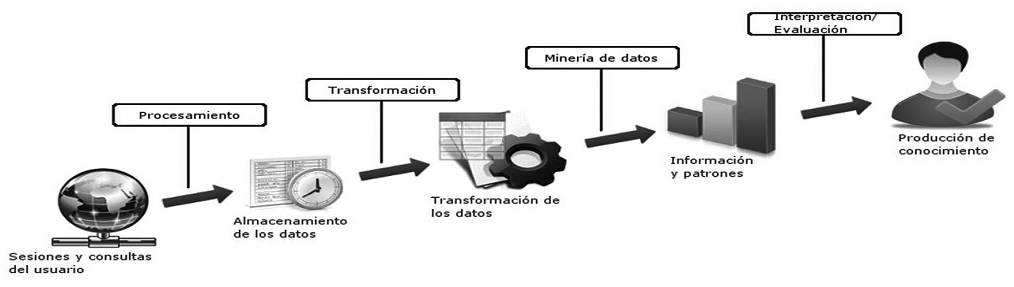
\includegraphics[width=10cm,height=5cm] {kdd.png} 
\caption[Proceso KDD]{Proceso KDD~\footnote{Imagen extraída de http://www.scielo.org.co articulo ``Aplicación del proceso de KDD en el contexto de bibliomining: El caso Elogim''}}
\label{fig:kdd}
\end{minipage}
\end{figure}

\subsection{Fases del Descubrimiento del Conocimiento}

El proceso KDD puede ser representado en 7 objetivos, los cuales se logran en diferentes fases, estos objetivos son:

\begin{enumerate}
    \item Determinar las fuentes de información que pueden ser útiles y dónde conseguirlas.
    \item Diseñar un esquema de almacenamiento de datos, un Data Warehouse.
    \item Implementación del almacén de datos que permita la navegación y visualización previa de los datos para el análisis.
    \item Selección, limpieza y transformación de los datos a analizar.
    \item Seleccionar y aplicar el método de minería de datos apropiado.
    \item Evaluación, interpretación, transformación y representación de los patrones extraídos.
    \item Difusión y uso del nuevo conocimiento.
    
\end{enumerate}

\subsubsection{Recogida de Datos}

La primeras fases del KDD determinan que las fases sucesivas sean capaces de extraer conocimiento válido y útil a partir de la información original.\\

En la fase de recogida de datos se sigue los siguientes pasos:

\begin{itemize}
    \item Selección de datos: 
    Por lo general la información que se quiere investigar sobre un cierto dominio de la organización se encuentra en bases de datos y fuentes internas como externas.
    \item Pre-proceso o limpieza de datos:
    En este paso se debe eliminar el mayor número de datos erróneos o inconsistentes e irrelevantes, esto también se conoce como limpieza y selección.
    \item Transformación de datos:
    Una vez limpiados y seleccionados los datos, se realiza un proceso de transformación que permite homologar la información, dando como resultado un conjunto de filas y columnas denominado ``Vista Minable'', con el fin de dejar los datos preparados para la modelización.
\end{itemize}

\subsubsection{Modelamiento}

El modelamiento o minería de datos es la etapa principal del KDD, aquí se determinan patrones y modelos para descubrir el conocimiento. Existen dos tipos de modelos y diferentes tareas para cada modelo.

\begin{enumerate}
    \item Tareas del Modelo Predictivo\\
    Son aquellas que buscan patrones que ayuden a predecir el comportamiento o tendencia de uno o varios valores.\\
    
    \begin{itemize}
        \item Clasificación:
        Los datos o registros son agrupados en clases, los cuales pueden tomar valores discretos. Su objetivo es determinar patrones en los registros, para identificar o predecir a que clase pertenecen los registros nuevos.
        
        \item Regresión:
        Se usa una regresión para predecir los valores ausentes de una variable basándose en su relación con otras variables del conjunto de datos.
    \end{itemize}
    
    \item Tareas del Modelo Descriptivo\\
    Son aquellas que exploran las propiedades de los datos analizados para encontrar patrones entre ellos.\\
    
    \begin{itemize}
        \item Agrupamiento (Clasificación no supervisada):
        Es similar a la clasificación, excepto que los grupos no son predefinidos. El objetivo es segmentar un conjunto de datos en grupos que pueden ser disjuntos o no. Los grupos se forman basados en la similaridad de los datos en ciertas variables. Como los grupos no son dados a priori se debe dar una interpretación de los grupos que se forman.
        
        \item Correlaciones:
        Identifica el grado de similitud de dos variables numéricas.
        \item Asociación:
        Las asociaciones entre dos atributos ocurre cuando la frecuencia de que se den dos valores determinados de cada uno conjuntamente es relativamente alta.
        \item Reglas de asociación secuenciales:
        Es una variante de asociación que utiliza la variable tiempo para identificar correlación.

        
    \end{itemize}
    
\end{enumerate}


Para estos modelos y tareas existen diferentes técnicas de minería de datos las cuales se pueden aplicar, a continuación se muestra un cuadro de las técnicas y tareas que utilizan, Figura \ref{fig:tecnicas}


\begin{figure}[H]
\begin{minipage}{\textwidth} 
\centering 
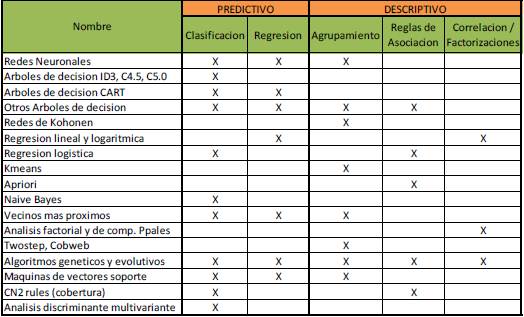
\includegraphics[width=12cm,height=7cm] {tecnicas.png}
\caption[Técnicas de minería de datos]{Técnicas de minería de datos~\footnote{Imagen extraída del libro ``Introducción a la Minería de Datos'', pag. 148, cap. 6}}
\label{fig:tecnicas}
\end{minipage}
\end{figure}

\subsubsection{Evaluación}

La fase de evaluación tiene como objetivo probar y validar el modelo creado en las fases anteriores. Para realizar las pruebas del modelo, se divide el set de datos en dos grupos, un grupo de entrenamiento de los datos, que ayuda a identificar la predicción que se espera, y el otro grupo es de prueba se valida la predicción y se analiza el porcentaje de acierto de dicha predicción. Por lo general se obtienen varios modelos aplicando las diferentes técnicas de minería de datos, los cuales son comparados buscando aquel que se ajuste mejor al problema. Si ninguno de los modelos alcanza los resultados esperados, debe
alterarse alguno de los pasos anteriores para generar nuevos modelos.

\section{Técnicas de Minería de Datos}

En el capitulo anterior se explico que existen diferentes técnicas y tareas en minería de datos para los distintos tipos de modelamiento.\\

El modelamiento acorde a este trabajo, corresponde a un modelo predictivo, en el cual se utilizarán cuatro técnicas en \textit{RapidMiner}, para generar cuatro modelos, estas técnicas son:\\

\begin{itemize}
	\item Regresión Lineal:\\
Es una técnica utilizada para la predicción numérica. Es una medida estadística que determina la relación ente una variable dependiente y una serie de variables independientes.\\
La regresión lineal intenta modelar la relación entre una variable escalar y una o más variables explicativas ajustando una ecuación lineal a los datos observados. Por ejemplo, uno podría querer relacionar los pesos de los individuos con sus alturas usando un modelo de regresión lineal \cite{rl}.

	\item Árboles de decisión:\\

Es una representación de datos que tiene forma de árbol invertido, donde sus nodos raíces están en la parte superior, creciendo hacia abajo.\\
Su objetivo es predecir el valor de un atributo destino (generalmente llamado clase o etiqueta) basándose en varios atributos de entrada, cada nodo interior del árbol corresponde a uno de los atributos de entrada. El número de aristas de un nodo interior nominal es igual al número de valores posibles del atributo de entrada correspondiente. Los bordes salientes de los atributos numéricos están etiquetados con rangos disjuntos. Cada nodo de hoja representa un valor del atributo de etiqueta dado los valores de los atributos de entrada representados por el camino de la raíz a la hoja \cite{ad}.
	\item Redes Neuronales:\\

Una red neuronal, es un modelo matemático o modelo computacional que se inspira en la estructura y aspectos funcionales de las redes neuronales biológicas. Una red neuronal consiste en un grupo interconectado de neuronas artificiales, y procesa la información utilizando un enfoque conexionista a la computación (el principio conexionista central es que los fenómenos mentales pueden ser descritos por redes interconectadas de unidades simples ya menudo uniformes). En la mayoría de los casos, una red neuronal es un sistema adaptativo que cambia su estructura basada en información externa o interna que fluye a través de la red durante la fase de aprendizaje. Las redes neuronales modernas suelen usarse para modelar relaciones complejas entre entradas y salidas o para encontrar patrones en los datos \cite{redn}.

	\item Máquinas de Vectores de Soporte (SVN):\\

Las máquinas de vectores de soporte estándar toman un conjunto de datos de entrada y predice, para cada entrada dada, cuál de las dos clases posibles comprende la entrada, haciendo del SVM un clasificador binario no probabilístico lineal. Dado un conjunto de ejemplos de entrenamiento, cada uno marcado como pertenecientes a una de dos categorías, un algoritmo de entrenamiento de SVM construye un modelo que asigna nuevos ejemplos en una categoría u otra. Un modelo SVM es una representación de los ejemplos como puntos en el espacio, mapeados de modo que los ejemplos de las categorías separadas se dividan por una brecha clara que es lo más amplia posible. Nuevos ejemplos se asignan a ese mismo espacio y se predice que pertenecen a una categoría basada en qué lado de la brecha en la que caen \cite{svn}.

\end{itemize}  

\section{RapidMiner}

RapidMiner es una herramienta de código abierto, usado para la minería de datos. Utiliza un ambiente gráfico que permite combinar distintos operadores y generar procesos de tratamiento y/o análisis de datos\\

\section{Conclusiones Marco Teórico}

A partir del estudio de la deserción según estadísticas del SIES, el tema de deserción universitaria, no es un fenómeno aislado, aproximadamente el 50 \%  de los alumnos que ingresan a un programa de estudios universitario, no termina la carrera, preocupando a varios actores del sistema.\\

Los datos recopilados por el SIES, orientan en cierto sentido el panorama que se a presentado entre los años 2010 y 2014 sobre el tema deserción, tomando variables globales como institución, género, jornada, establecimiento de origen y acreditación.\\

El concepto de inteligencia del cliente, entrega herramientas para analizar las necesidades y relacionamiento que tiene el alumno con la universidad, esto ayudará para identificar a través de entrevistas, variables influyentes en continuar y/o desertar de la carrera. Las variables determinadas ayudarán al proceso de inteligencia de negocio, las cuales serán extraídas, transformadas y cargadas en una base analítica, para finalizar aplicando el concepto minería de datos y generar los modelos con la herramienta RapidMiner.













% \chapter[Técnicas de Minería de Datos]{Técnicas de Minería de Datos}
\label{ch:tecdm}


\part{Desarrollo}
\chapter[Inteligencia del Cliente al Tema Deserción]{Inteligencia del Cliente al Tema Deserción}
\label{ch:des}


Un aspecto importante del concepto de Inteligencia del Cliente, es entender las necesidades del consumidor. En el caso de este trabajo, se manejan los conceptos de IC aplicado a alumnos, para entender sus necesidades y motivaciones en terminar una carrera universitaria.\\

El siguiente desarrollo busca como objetivo ver las motivaciones de los alumnos, para convertirlos en constructos junto a sus asociaciones, los cuales entregarán métricas y variables para analizar el tema deserción. Las métricas y variables definidas en esta sección, ayudará a la selección de datos y construcción de los modelos, para luego aplicar las técnicas de minería de datos con la herramienta \textit{RapidMiner} a la base de datos de la entidad  privada.

\section{Entrevistas con Metodología de Metáforas}


Para captar las necesidades de los alumnos se utilizó la metodología de metáforas, en donde se le pide al entrevistado que recorte de 6 a 8 imágenes de revistas que representen para él, el concepto a evaluar. El concepto a evaluar en este caso, se representa con la pregunta principal ¿Qué te motiva a terminar la carrera? (Ver Anexo A).\\

El marco muestral se define a partir de un segmento de cliente, para el caso de esta investigación, el segmento abarca a alumnos de educación superior de instituciones universitarias.\\

Como el objetivo de las entrevistas es encontrar las necesidades y motivaciones de los alumnos, se utilizó un muestreo no probabilístico, del tipo intencional o por conveniencia, que consiste en seleccionar individuos que son más fáciles de entrevistar \cite{muestra}.\\

\begin{table}[H]
	\begin{center}
\begin{tabular}{|c|c|c|c|c|c|}
	\hline
	Carrera & Cantidad & Hombre & Mujer & Edad Promedio  & Año de Carrera Promedio  \\
	\hline \hline
	Ing. Informática & 7 & 7 & 0 & 25 & 4to \\ \hline
    Ing. Industrial & 9 & 5 & 4 & 21 & 2do \\ \hline
    Ing. Obras Civiles & 2 & 2 & 0 & 19 & 2do \\ \hline
    Ing. Comercial & 2 & 1 & 1 & 23 & 3er \\ \hline
    Psicología & 2 & 2 & 0 & 24 & 5to \\ \hline \hline
    Total & 22 & 17 & 5 & 22 & 3er \\ \hline \hline
\end{tabular}
\caption{Tabla resumen de muestra}
	\label{tabla:resumenmuestra}
\end{center}
\end{table}

El resultado de las entrevistas se muestra en la tabla resumen (Tabla \ref{tabla:resumenmuestra}), estás entrevistas derivan a constructos a partir de sus necesidades y motivaciones.\\



\subsection{Constructos}

Los constructos son definiciones interpretadas a partir de las asociaciones de las imágenes escogidas por los entrevistados, estas definiciones derivan en variables a contemplar para armar un modelo.\\ 

Los constructos recogidos en esta investigación reflejan el sentir del alumno en la carrera, los cuales se pueden plasmar en su formación como profesional y en sus sueños futuros.\\

\begin{figure}[H]
		\centering 
		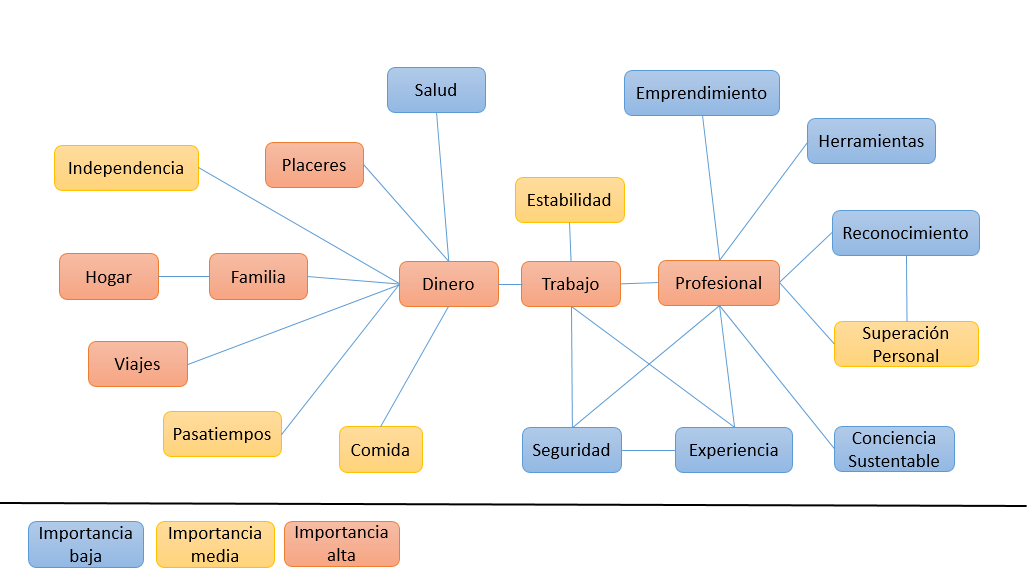
\includegraphics[width=12cm,height=7cm] {constructos.png} 
		\caption[Mapa de Consenso Generado]{Mapa de Consenso Generado}
		\label{fig:constru}
\end{figure}  

La Figura \ref{fig:constru} representa el \textit{Mapa de Consenso} generado a partir de los constructos obtenidos de las entrevistas, los más importantes son los que se repitieron en la mayoría de las entrevistas y son los principales insight de los alumnos al responder la pregunta ¿Qué te motiva a terminar la carrera?.\\

A continuación, se detallan los constructos obtenidos, en donde las asociaciones son realizadas por los entrevistados, las definiciones son interpretaciones a las asociaciones, y las variables son los posibles datos ligados a las definiciones.\\    

\underline {Constructo 1 - Familia} \\
Asociaciones:
\begin{enumerate}
	\item Representa el compartir con la familia una situación económica estable.
	\item Tener una familia y tener dinero para mantener a la familia.
	\item El terminar una carrera implica tener un buen trabajo y mucho dinero, con el cual se puede optar a mejores condiciones de vida.
	\item Poder dar una buena educación a los hijos.
	\item Poder formar mi familia alegre y saludable.	
\end{enumerate}

Definición:\\
Un alumno que valore la familia, también valorará el tiempo que tiene para dedicar a esta, mientras estudia.\\
Un alumno que vive en comunas apartadas tendrá menos tiempo con la familia, lo que redunda en buscar lugares más cercanos.\\
Por otro lado, es importante clasificar las carreras que otorgan un mayor bienestar para la familia.\\
Sumado a lo anterior de igual forma se debe analiza el impacto que tiene el deseo de estudiar la carrera.\\


Variables:
\begin{itemize}
	\item Distancia a universidad (comuna).
	\item Prioridad de postulación a carrera
	\item Tiempo medio de encontrar trabajo estudiante egresado.
\end{itemize}


\underline {Constructo 2 - Independencia}\\ 
Asociaciones:
\begin{enumerate}
	\item Tener un espacio personal grande y vanguardista.
	\item Tener un auto para tener independencia.
	\item Tener la autonomía de vivir solo y tener un hogar
	\item Trabajar de forma independiente
	\item Poder vivir sola y tener mi departamento.	
\end{enumerate}

Definición:\\
Un alumno que valora la independencia, se encuentra más dispuesto a conseguir beneficios que lo ayuden económicamente, así como también trabajar durante la etapa estudiantil para satisfacer sus necesidades.\\

Variables:
\begin{itemize}
	\item Becas
	\item Créditos
	\item Beca alimenticia (Junaeb)
	\item Trabajador
\end{itemize}

\underline {Constructo 3 - Dinero}\\ 
Asociaciones:
\begin{enumerate}
	\item Representa el vehículo que podría adquirir teniendo recursos
	\item Felicidad y estabilidad amorosa, gracias a una buena situación económica.
	\item Poder acceder a muchas cosas, como bienes
	\item Poder comprar tecnología, gracias al buen sueldo que tendré
	\item Ser un profesional significa poder tener mucho dinero
\end{enumerate}

Definición:\\
Un alumno que tome en cuenta el dinero que ganará luego de egresar, debe tener conciencia en las estadísticas de su carrera, cual es la tasa de empleabilidad al 1er año de egreso y como aumentará su sueldo con los años de experiencia.\\

Variables:
\begin{itemize}
	\item Empleabilidad al 1er año
	\item Ingreso promedio al 4to año	
\end{itemize} 

\underline {Constructo 4 - Placeres}\\ 
Asociaciones:
\begin{enumerate}
	\item Tener un título, se asocia a disfrutar placeres de la vida.
	\item Representa las comodidades que uno podría tener una vez trabajando.	
	\item Poder obtener gustos exclusivos gracias al dinero.
	\item Comprar cosas exclusivas
\end{enumerate}

Definición:\\
Hace referencia a la libertad de poder gastar el dinero ganado en cosas o experiencias satisfactorias. Este constructo se encuentra asociado al constructo de Dinero, por lo que se aplican las mismas variables.\\

Variables:
\begin{itemize}
	\item Empleabilidad al 1er año
	\item Ingreso promedio al 4to año	
\end{itemize}


\underline {Constructo 5 - Trabajo} \\
Asociaciones:
\begin{enumerate}
	\item Trabajar de forma relajada, ya que con el título tienes una base para dedicarse a lo que te gusta.
	\item Representa la adquisición de un bien raíz gracias al trabajo después de titulado
	\item Es lo que quiero llegar hacer, y tener un trabajo luego de titularme.	
	\item Poder relacionarse con otras personas y poder tener un trabajo sinérgico
\end{enumerate}

Definición:\\
Representa a lo que se dedicará y obtendrá el alumno una vez titulado. Se relaciona al constructo Dinero y se asocian las mismas variables.\\

Variables:
\begin{itemize}
	\item Empleabilidad al 1er año
	\item Ingreso promedio al 4to año	
\end{itemize}


\underline {Constructo 6 - Profesional} \\
Asociaciones:
\begin{enumerate}
	\item Generar aportes al trabajo, ser un buen profesional
	\item Tener un trabajo relacionado en redes informáticas y ser un buen profesional, para viajar por el mundo
	\item Encontrar un trabajo en una empresa prestigiosa.	
	\item Es a lo que uno aspira ser como ingeniero, teniendo buen puesto y reputación.
	\item Poder dedicarme al desarrollo de aplicaciones móviles.
\end{enumerate}

Definición:\\
Un alumno que valora el ser un profesional, tomará en cuenta el prestigio y excelencia de la institución, como también su formación profesional, por lo que será interesante saber si la institución se encuentra acreditada y si el alumno participa o ha participado en actividades que ayuden a validar sus capacidades.\\

Variables:
\begin{itemize}
	\item Acreditación Institucional
	\item Carrera Acreditada
	\item Talleres de Certificación
	\item Talleres de Desarrollo Profesional	
\end{itemize} 


\underline {Constructo 7 - Viajes} \\
Asociaciones:
\begin{enumerate}
	\item Tener la disponibilidad de tiempo y dinero, salir de la rutina, tener una vida más relajada
	\item Después de la carrera hay tiempo para disfrutar y conocer el mundo. 
	\item Libertad en poder ir a lugares diferentes y con mucha naturaleza
	\item Sin dinero no se puede viajar, y teniendo una carrera, uno puede ganar mucho dinero.	
	\item Poder viajar y hospedarse en buenos hoteles
\end{enumerate}

Definición:\\
Representa la libertad y la posibilidad de poder conocer nuevos lugares, sin preocupaciones de dinero.\\

Los viajes para los entrevistados representan el conocer otros países, si bien hace referencia a algo más vacacional, se puede asociar con las diferentes oportunidades que puede otorgar la institución para realizar intercambios, más puntual si el alumno ha realizado un intercambio por medio de la institución.\\

Variables:
\begin{itemize}
	\item Alumno realizo intercambio
\end{itemize}



\underline {Constructo 8 - Pasatiempos} \\
Asociaciones:
\begin{enumerate}
	\item Tener una buena situación económica para disfrutar eventos culturales.
	\item Tener muchos libros por el gusto de leer.
	\item Poder tener la libertad de darse tiempos libres y hacer las cosas que uno quiere.
	\item Dedicar tiempo para mi persona y realizar lo que me gusta, la cocina.	
	\item Representa la parte artística que podría dedicarme teniendo recursos.
\end{enumerate}

Definición:\\
Hace referencia al tiempo disponible que tendrá, a poder cumplir y hacer lo que siempre le ha gustado hacer. Es importante para el alumno, que la institución a la cual pertenece disponga de talleres o facilidades que complementen sus estudios con los pasatiempos y si el alumno participa activamente de algún taller proporcionado por la institución.\\


Variables:
\begin{itemize}
	\item Taller deportivo o cultural 
	\item Beca deportiva
\end{itemize}


\underline {Constructo 9 - Hogar} \\
Asociaciones:
\begin{enumerate}
	\item Representa el compartir con la familia una situación económica estable.
	\item Tener una familia y tener dinero para mantener a la familia.
	\item Poder acceder a una buena casa en un buen barrio
	\item Tener una casa amplia y con bonita vista para recibir a la familia	
\end{enumerate}

Definición:\\
Representa independencia y unión familiar a través de la estabilidad económica. Se asocia a los constructos de Dinero y Familia\\

Variables:
\begin{itemize}
	\item Empleabilidad al 1er año
	\item Ingreso promedio al 4to año
	\item Distancia a universidad (comuna).
	\item Estudiar 3 primeras prioridades.
	\item Tiempo medio de encontrar trabajo estudiante egresado.	
\end{itemize} 

\underline {Constructo 10 - Comida} \\
Asociaciones:
\begin{enumerate}
	\item Tener una buena situación económica.
	\item Tener para comer y una vida sana.
	\item Representa los gustos que me podría dar, teniendo recursos.	
	\item Tener gustos sin depender económicamente de otras personas
	\item Tener un lugar agradable dentro de la casa
\end{enumerate}

Definición:\\

Hace mención a satisfacer la necesidad de alimento y darse una buena vida. Se asocia al constructo de Dinero junto a sus variables.\\

Variables:
\begin{itemize}
	\item Empleabilidad al 1er año
	\item Ingreso promedio al 4to año
	\item Beca alimenticia
\end{itemize} 

\underline {Constructo 11 - Experiencia} \\
Asociaciones:
\begin{enumerate}
	\item Estar listo para enfrentar el mundo laboral.
	\item Un profesional termina las cosas de manera más rápida, porque está preparado.	
\end{enumerate}

Definición:\\

Hace referencia a sentirse preparado, a estar seguro en lo que se trabaja y poder cumplir de manera excelente. Es importante para el alumno ver la vinculación con el medio que tiene la institución y las prácticas ofrecidas.\\

Variables:
\begin{itemize}
	\item Prácticas realizadas
	\item Taller de Desarrollo Profesional	
\end{itemize}


\underline {Constructo 12 - Superación personal} \\
Asociaciones:
\begin{enumerate}
	\item Cerrar una etapa de la vida, para pasar a una siguiente.
	\item Significa el cierre y el comienzo de una nueva etapa.
	\item Terminar una carrera transmite seguridad y sentirse útil para algo.
	\item Representa crecimiento personal y laboral	.
	\item Es el logro de cumplir con el objetivo de ser ingeniero.
\end{enumerate}

Definición:\\
Representa el alcanzar una meta, crecer, ser independiente y seguro. Esto se puede representar por los logros alcanzados por el alumno, como la cantidad de ramos aprobados en un semestre, promedio de notas o posición en ranking de alumno.\\

Variables:
\begin{itemize}
	\item Porcentaje ramos aprobados
	\item Promedio de notas
	\item Ranking del alumno	
\end{itemize} 

\underline {Constructo 13 - Salud} \\
Asociaciones:
\begin{enumerate}
	\item Poder tener el dinero para obtener buenos tratamientos médicos		
\end{enumerate}

Definición:\\
Tener un título implica poder a acceder a una salud de calidad. Se asocia al constructo Dinero junto a sus variables.\\

Variables:
\begin{itemize}
	\item Empleabilidad al 1er año
	\item Ingreso promedio al 4to año	
\end{itemize}



\underline {Constructo 14 - Seguridad} \\
Asociaciones:
\begin{enumerate}
	\item Desarrollar seguridad personal
	\item Tener una carrera te da seguridad de tener un buen trabajo	
	\item Salir de la carrera es un gran paso y te da libertar y seguridad en trabajar en lo que quieras
\end{enumerate}

Definición:\\
Hace referencia a que un título certifica las capacidades de una persona, haciéndolas sentir más seguras. Un alumno que busca seguridad laboral, buscara mejorar sus capacidades con certificaciones, es importante entonces que la institución a la que pertenece certifique los conocimientos del alumno.\\

Variables:
\begin{itemize}
	\item Talleres de certificación
	\item Acreditación institucional
	\item Carrera acreditada	
\end{itemize}


\underline {Constructo 15 - Conciencia sustentable} \\
Asociaciones:
\begin{enumerate}
	\item Vida consciente con el planeta, a largo plazo
	\item Crear una fundación para ayudar a niños con discapacidad	
	\item Me gustaría tener un desarrollo sustentable, poder ayudar a la naturaleza con mi carrera
\end{enumerate}

Definición:\\
Se refiere a que una carrera entrega nociones y entendimiento sobre los efectos que tienen diferentes efectos sobre el planeta y la sociedad.\\  

Variables:
\begin{itemize}
	\item Participación en voluntariado social o ONG
	\item Ramos relacionado a conciencia sustentable	
\end{itemize} 

\underline {Constructo 16 - Reconocimiento} \\
Asociaciones:
\begin{enumerate}
	\item Representa el triunfo que puede llegar a tener como profesional.
	\item Terminar la carrera, da una sensación de libertad y triunfo. 
	\item Estar graduado y ser reconocido como un ingeniero.
	\item Como te observan las otras personas y como me proyecto como profesional	
	\item Refleja a mis padres, al terminar mi carrera ellos estarían orgullosos de mí
\end{enumerate}

Definición:\\
Representa a la sensación de un buen estatus, de crecimiento y aceptación. Se asocia al constructo Superación Personal junto a sus variables.\\

Variables:
\begin{itemize}
	\item Porcentaje ramos aprobados
	\item Promedio de notas
	\item Ranking del alumno	
\end{itemize} 

\underline {Constructo 17 - Emprendimiento} \\
Asociaciones:
\begin{enumerate}
	\item Poder sacar un postgrado
	\item Poder dar clases en un futuro.
	\item Tener tiempo para poder realizar un curso de inglés y viajar al extranjero.
	\item Poder emprender con un negocio gourmet
	\item Tener mi propia oficina, trabajar con más gente y enseñar lo que sé	
\end{enumerate}

Definición:\\
Representa los sueños a futuros que se pueden cumplir gracias a un título. Para este constructo se relaciona la participación del alumno en distintas actividades que se relacione a emprendimiento, como talleres o concursos a través de la institución a la que pertenece.\\

Variables:
\begin{itemize}
	\item Talleres de emprendimiento	
\end{itemize}


\underline {Constructo 18 - Estabilidad} \\
Asociaciones:
\begin{enumerate}
	\item Generar estabilidad y buenos lazos.
	\item Trabajar con personas, tener vida social 	
	\item Poder tener estabilidad económica y por ende tranquilidad
\end{enumerate}

Definición:\\
Representa que un título otorga poder estar seguro tanto económicamente como emocional. Un alumno con interés en tener una estabilidad económica como emocional, participara de actividades que lo ayuden a encontrar esa estabilidad, por ende, las instituciones deben tener estas actividades, y el alumno participar de dichas actividades.\\

Variables:
\begin{itemize}
	\item Talleres Bienestar estudiantil
	\item Talleres de Desarrollo Profesional	
\end{itemize}


\underline {Constructo 19 - Herramientas} \\
Asociaciones:
\begin{enumerate}
	\item Sueños de ser papá, de tener las herramientas para dar un buen pasar
	\item Los profesores motivan y te enseñan hacer trabajos de calidad	
	\item La universidad me da herramientas que me servirán para el futuro
	\item Representa las habilidades obtenidas en la carrera
\end{enumerate}

Definición:\\
Hace referencia al aprendizaje obtenido en la etapa universitaria. Es importante para el alumno tener las capacidades suficientes para poder ejercer sin problemas su título, por ende, participara en actividades que le brinden estas herramientas.\\

Variables:
\begin{itemize}
	\item Talleres de certificación
	\item Talleres de Desarrollo Profesional	
\end{itemize}


\subsection{Tabla de los Constructos}

\begin{longtable}{| p{4cm}| p{8cm} |}
	\hline
	Variable & Descripción \\
	\hline \hline
	\endfirsthead	
	\hline
	Variable & Descripción \\
	\hline \hline
	\endhead
		
	\multicolumn{2}{|c|}{Institución y Carrera} \\ \hline
	\hline
	Distancia casa - institución & Distancia en kilómetros \\ \hline
Empleabilidad al 1er año  & Porcentaje de egresados con trabajo al 1er año \\ \hline
Ingreso promedio 4to año & Cantidad de dinero a ganar al 4to año de experiencia laboral  \\ \hline
Acreditación Institucional & Indica si la institución se encuentra acreditada\\ \hline
Carrera acreditada & Indica si la carrera se encuentra acreditada \\ \hline 
\hline
\multicolumn{2}{|c|}{Desempeño Alumno} \\ \hline
\hline	
Beca deportiva & Indica si el alumno tiene beca deportiva\\ \hline
Beca de estudio  & Indica si el alumno tiene beca de estudio\\ \hline
Beca de alimento & Indica si el alumno tiene beca de alimento\\ \hline
Crédito  & Indica si el alumno tiene crédito\\ \hline
Promedio notas acumuladas & Promedio total de todas las notas del alumno en la carrera\\ \hline    
Ranking del alumno & Posición del alumno en la carrera\\ \hline
Prácticas & Cantidad de prácticas realizadas por el alumno\\ \hline 
Porcentaje ramos aprobados & Índice de aprobación del alumno, sacado de todos los ramos cursados\\ \hline
\hline
\multicolumn{2}{|c|}{Motivaciones del Alumno} \\ \hline
\hline	   
Prioridad de postulación a carrera  & Lugar en el orden de postulación a su actual carrera\\ \hline
Trabajador &  Indica si el alumno se encuentra trabajando\\ \hline 
Taller emprendimiento  & Indica si el alumno ha realizado talleres o cursos relacionado a emprendimientos\\ \hline
Taller bienestar estudiantil & Indica si el alumno ha participado en talleres que ayuden a su estabilidad emocional o de desempeño en la institución\\ \hline		
Taller profesional  & Indica si el alumno ha participado en talleres que ayuden a su futuro profesional\\ \hline
Intercambio estudiantil & Indica si el alumno ha realizado un intercambio\\ \hline
Taller certificación & Indica si el alumno ha participado en talleres que certifiquen sus conocimientos \\ \hline
Taller deportivo o cultural &  Indica si el alumno ha participado en talleres o ramos de tipo deportivo o cultural\\ \hline
Voluntariado social  & Indica si el alumno ha realizado un voluntariado social o participado en una ONG\\ \hline

	
	\caption{Tabla de variables.}
	\label{tabla:Tablou de variables}
\end{longtable}	

Las variables derivadas del estudio de los 19 constructos generan la Tabla \ref{tabla:Tablou de variables} que se pueden ordenar en tres grupos, el primero ``Institución y Carrera'', el cual tiene información general de la institución y carrera. El segundo ``Desempeño Alumno'', el cual tiene información puntual del alumno sobre si posee beneficios y datos de su desempeño. El tercero ``Motivaciones del Alumno'', el cual tiene información puntual en la participación de diversas actividades que se asocian a sus motivaciones y a una orientación vocacional.\\


\chapter[Aplicando Minería de Datos con RapidMiner]{Aplicando Minería de Datos con RapidMiner}
\label{ch:desmin}

\section{Identificación de datos y variables}
\subsection{Datos}

Los datos a utilizar en los modelos a presentar en este capítulo son extraídos de la base de datos de la institución privada. Estos datos corresponde a información de los años 2014 y 2015 de alumnos de las distintas carreras de ingeniería que imparte la institución. Además se extrae información a través del SIES sobre la institución y sus diferentes carreras de ingeniería con respecto a acreditación e indices de empleabilidad.\\

\subsection{Variables}

Las variables consideradas en este estudio, corresponden al análisis de los constructos del capítulo anterior, además se consideran variables analizadas en el capítulo dos sobre la deserción en Chile.\\

Las variables obtenidas se dividen en tres principales grupos, la primera llamada ``Individual y Educación Media'', corresponde a datos del individuo como su edad y genero, e información previa al ingreso de una institución de educación superior. La segunda llamada ``Institución y Carrera'', corresponde a datos puntuales de la institución y carrera. La tercera llamada ``Alumno'', corresponde a datos sobre actividades, beneficios y rendimiento del alumno.\\



\begin{longtable}{|l|l|l|}
			\hline
			Variable & Tipo & Descripción \\
			\hline \hline
			\endfirsthead
			
			\hline
            Variable & Tipo & Descripción \\
            \hline \hline
            \endhead
			
			\multicolumn{3}{c}{Individual y Educación Media} \\ \hline
			Distancia hogar-institución &  & \\ \hline
			Genero &  & \\ \hline
			Edad &  & \\ \hline
			Tipo establecimiento de origen &  & \\ \hline
			Notas enseñanza media & & \\ \hline
			Promedio PSU lenguaje y matemáticas &  & \\ \hline
			Prioridad de postulación a carrera & & \\ \hline
			Reingresante & & \\ \hline
			Trabajador & & \\ \hline 
			\multicolumn{3}{c}{Institución y Carrera} \\ \hline
			Tipo Institución &  & \\ \hline
			Acreditación Institucional &  & \\ \hline
			Jornada &  & \\ \hline
			Arancel anual & & \\ \hline
			Empleabilidad al 1er año & & \\ \hline
			Ingreso promedio 4to año & & \\ \hline
			Carrera acreditada & & \\ \hline 
			\multicolumn{3}{c}{Alumno} \\ \hline
			Semestres cursados & & \\ \hline
			Taller profesional realizados & & \\ \hline
			Ha realizado intercambio & & \\ \hline
			Taller certificación realizados & & \\ \hline
			Taller deportivo o cultural & & \\ \hline
			Tiene beca deportiva & & \\ \hline
			Tiene beca de estudio &  & \\ \hline
			Tiene beca de alimento & & \\ \hline
			Tiene crédito &  & \\ \hline
			Promedio notas acumuladas &  & \\ \hline
			Ramos aprobados por semestre & & \\ \hline
			Causales acumuladas & & \\ \hline
			Ranking del alumno & & \\ \hline
			Prácticas realizadas & & \\ \hline
			Ha realizado voluntariado social & & \\ \hline
		\caption{Tablou de variables.}
		\label{tabla:Tablou de variables}
\end{longtable}	

Las variables a considerar crean el tablou representado en la Tabla \ref{tabla:Tablou de variables}, estas variables serán rellenadas a partir de los datos de la institución privada.

\subsection{Modelamiento}

La construcción de los modelos se implementará con la herramienta \textit{RapidMiner} utilizando como entrada el tablou generado anteriormente.\\

La herramienta \textit{RapidMiner} permite a través de operadores, construir un proceso. Los procesos son una serie de pasos constituidos por operadores.\\

\begin{figure}[H]
	\centering 
	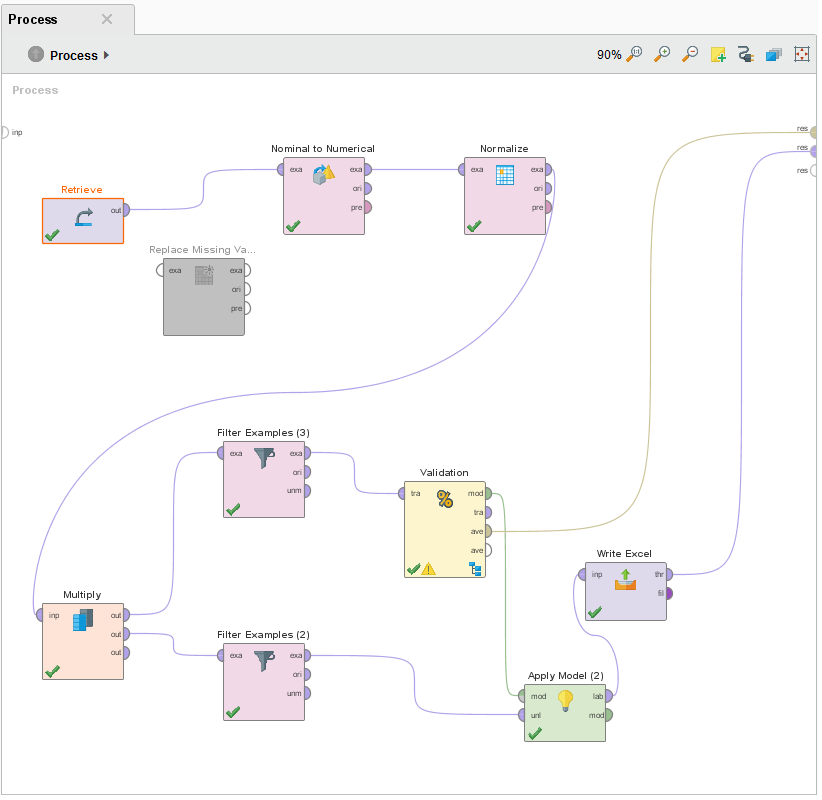
\includegraphics[width=12cm,height=7cm] {proceso.png} 
	\caption[Proceso de Predicción]{Proceso de Predicción}
	\label{fig:proceso}
\end{figure}

\begin{figure}[H]
	\centering 
	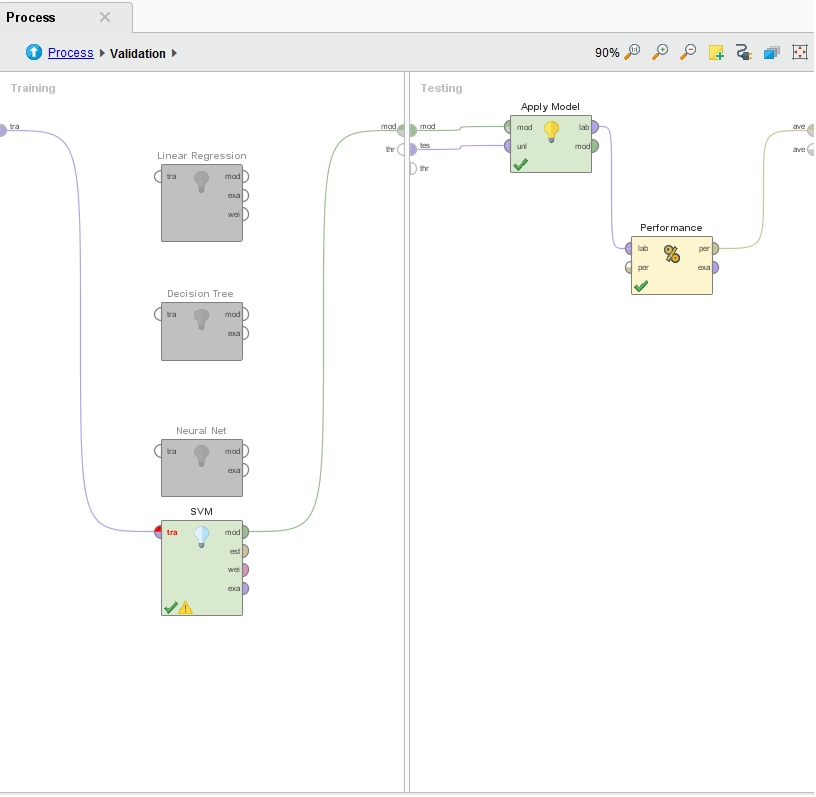
\includegraphics[width=12cm,height=7cm] {provalidacion.png} 
	\caption[Validación]{Validación}
	\label{fig:validacion}
\end{figure}
\part{Conclusiones}
\chapter[Conclusiones e Implementación]{Conclusiones e Implementación}
\label{ch:conclu}

\section{Conclusiones}
A partir del estudio de la deserción según estadísticas del SIES, el tema de deserción universitaria, no es un fenómeno aislado, aproximadamente el 50 \%  de los alumnos que ingresan a un programa de estudios universitario, no termina la carrera, preocupando a varios actores del sistema.\\

Los datos recopilados por el SIES, orientan en cierto sentido el panorama que se a presentado entre los años 2010 y 2014 sobre el tema deserción, tomando variables globales como institución, género, jornada, establecimiento de origen y acreditación.\\

El concepto de inteligencia del cliente, entrego herramientas para analizar las necesidades y relacionamiento que tiene el alumno con la universidad, esto ayudo a identificar a través de entrevistas, variables influyentes en continuar y/o desertar de la carrera. Las variables determinadas con inteligencia del cliente junto a las variables de información del SIES, ayudaron al proceso de inteligencia de negocio, las cuales fueron extraídas, transformadas y cargadas en una base analítica, para finalizar aplicando el concepto minería de datos y generar los modelos con la herramienta RapidMiner.\\

Si bien se generaron variables para un modelo con inteligencia del cliente, finalmente se utilizaron variables disponibles en los datos otorgados por la institución, las variables extraídas de estos datos fueron principalmente variables estudiadas en otras investigaciones respecto al tema deserción y que se comprobó su influencia en las técnicas de predicción.\\

Dentro de las cuatro técnicas probadas en los modelos generados para jornada Diurna y Vespertina, el que tuvo una mejor predicción en ambos modelos fue SVN, prediciendo el 100\% de las observaciones probadas, sin embargo seria optimo a futuro probar el modelo resultante de inteligencia del cliente y aplicar la siguiente implementación utilizando los pasos del modelamiento con la herramienta \textit{RapidMiner} con la técnica SVN.\\

\section{Implementación}

El primer paso es generar los procesos de minería de datos, esto quiere decir realizar actividades relacionadas con la automatización de estos procesos, por este motivo se considera las siguientes actividades:

\begin{enumerate}
	\item Recolectar información de las motivaciones del alumno al finalizar cada semestre.
	\item Definir el día de la extracción de la información, debiese ser finalizando las encuesta de fin de semestre.
	\item Automatizar la generación de la base de datos que alimentará el modelo propuesto. Se debe considerar proceso ETL.
	\item Procesar el modelo con la herramienta \textit{RapidMiner}.
	\item Integrar dichos resultados a un sistema que puede ser interno o externo a los sistemas de la institución. La herramienta \textit{RapidMiner} permite generar los resultados en archivos o integrarlos a una base de datos.
\end{enumerate}

Una vez que el modelo genere la información con los alumnos propensos a desertar de la carrera, esta información debe ser entregada a los entes o áreas de interés para que realicen las acciones necesarias para mantener al alumno en la institución, las cuales pueden vincularse a las actividades que se definieron como motivaciones del alumno en el modelo de la Tabla \ref{tabla:Tablou de variables}.

\part{Información Adicional}
% Iniciamos el resto de secciones adicionales al contenido: referencias y apendices
\backmatter


% Bibliografía
% referencias.bib es el archivo con la base de datos bibliografica
% se recomienda utilizar un manejador de referencias: Jabref (jabref.sourceforge.net)
% El estilo por defecto es IEEE Transactions
\bibliographystyle{IEEEtran}
% Acá puede incluir uno más archivos de referencia
\bibliography{IEEEabrv,referencias}


% Simbología y glosario
% Utilice un paquete para generar símbolos y glosarios.
% Por ejemplo: nomencl (http://texdoc.net/pkg/nomencl)


% Anexos
\appendix

% Aca se incluyen los archivos con el texto de los anexos
% Por ejemplo, anexo.tex
\chapter{Primer anexo}
\label{ch:anexo-a}
\newpage
%\blindtext[5]
\underline {ENTREVISTA 1} \\
Nombre: Marcel\\
Edad: 25\\
Carrera: 4to Año de Ingeniería Civil Informática y Telecomunicaciones\\
Comuna: Santiago Centro \\

\begin{table}[H]
\centering
\begin{tabular}{>{\centering\arraybackslash}m{1cm} >{\centering\arraybackslash}m{2cm} >{\arraybackslash}m{5cm}>{\arraybackslash}m{5cm}}
\hline
Número & Imagen & Descripción & Asociaciones \\
\hline \hline

1 & 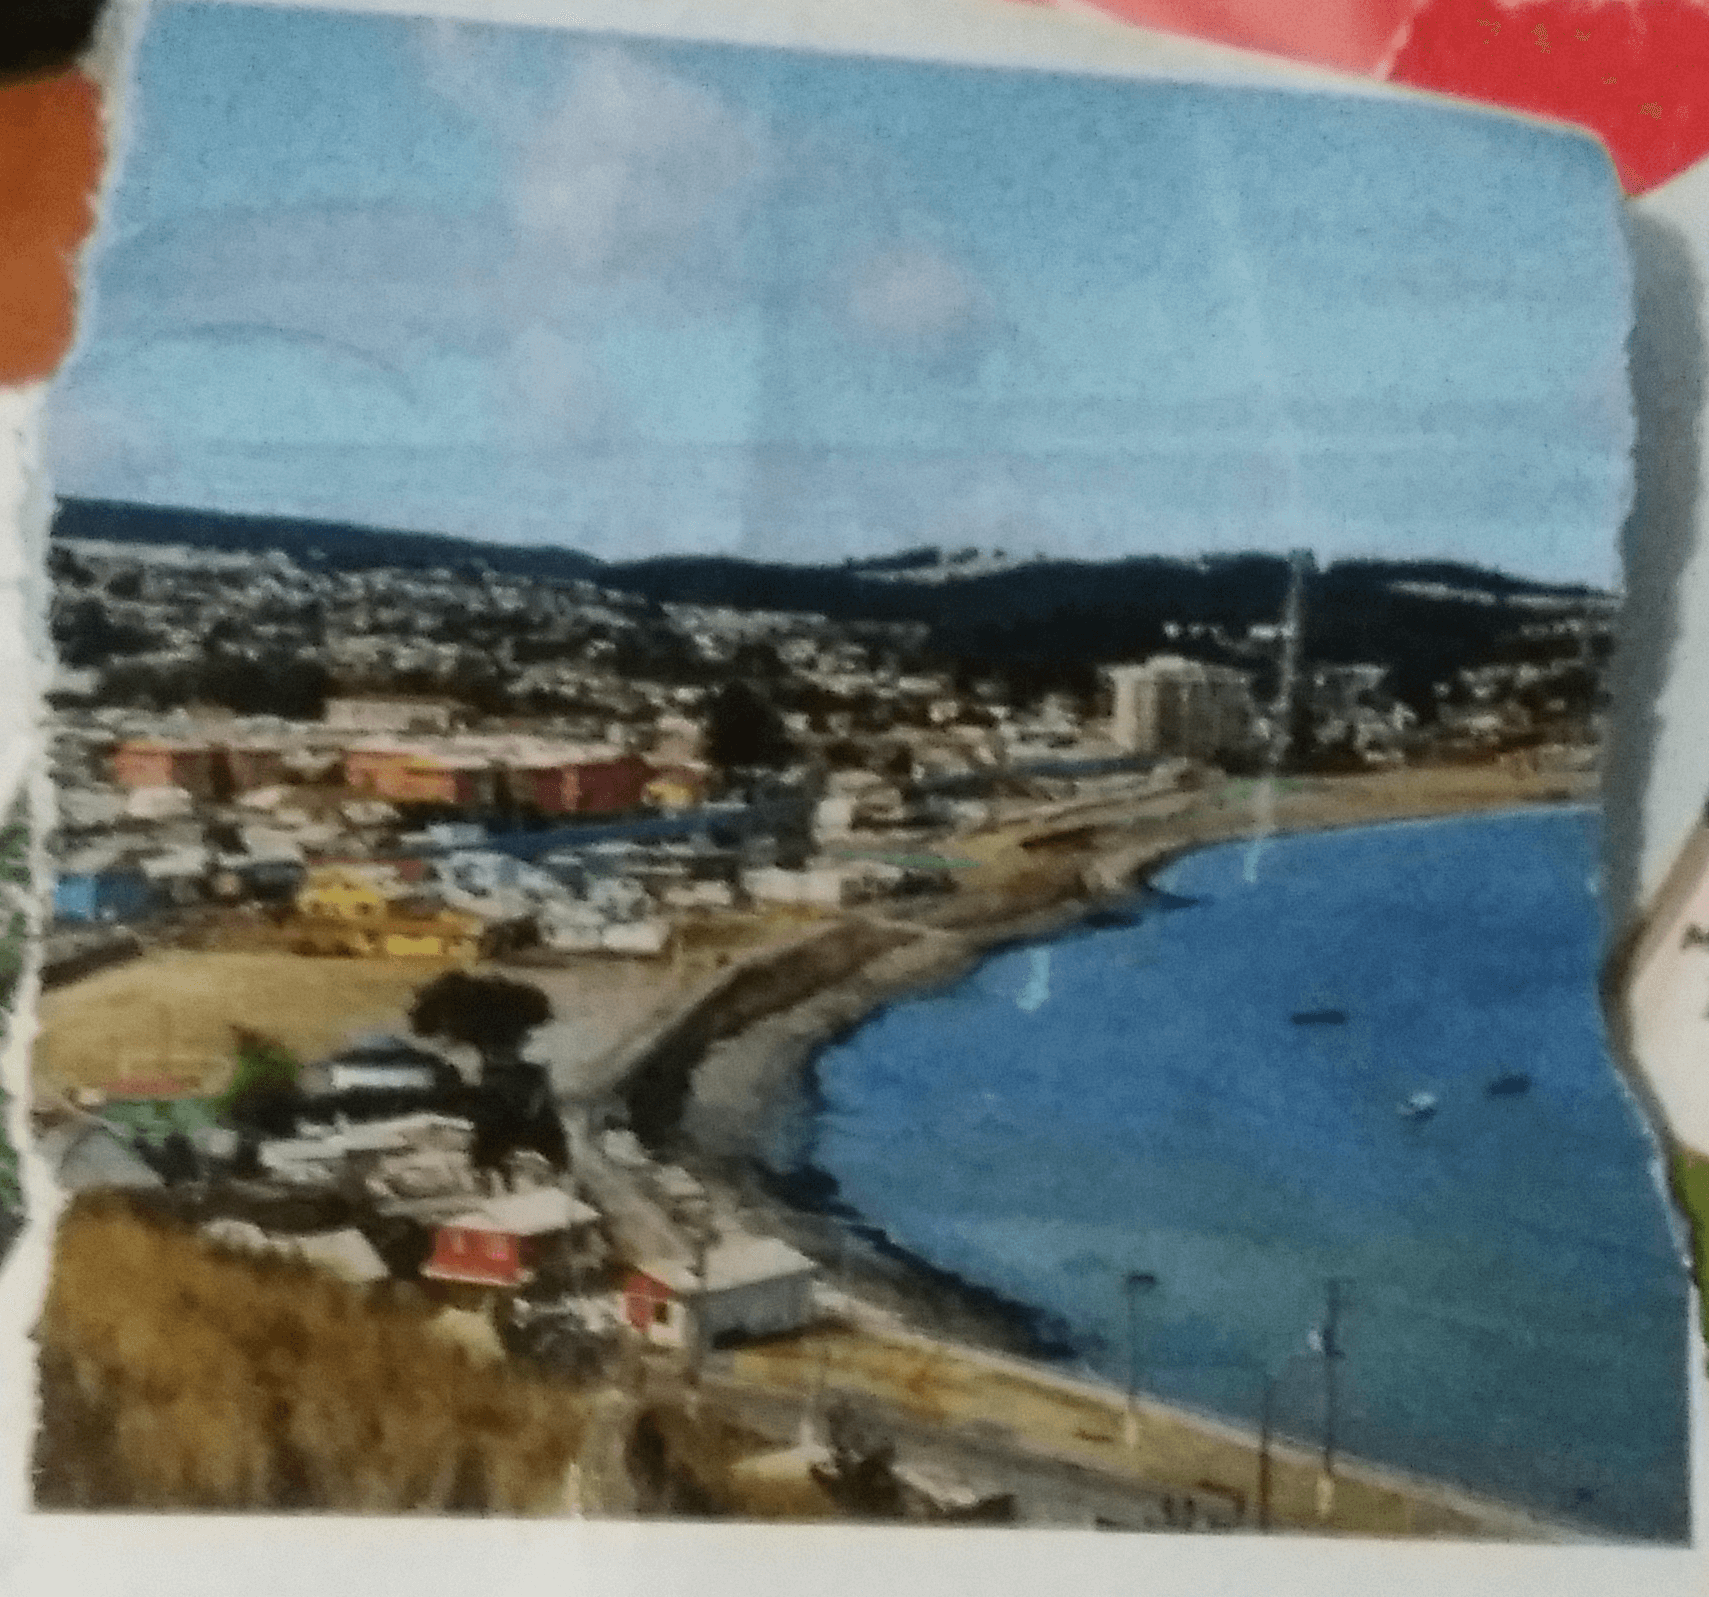
\includegraphics[width=20mm,height=20mm]{marcel1.png} & ``Una casa en la playa, ideal para pasear con la familia'' & ``Representa el compartir con la familia con una situación económica estable'' \\
\hline

2 & 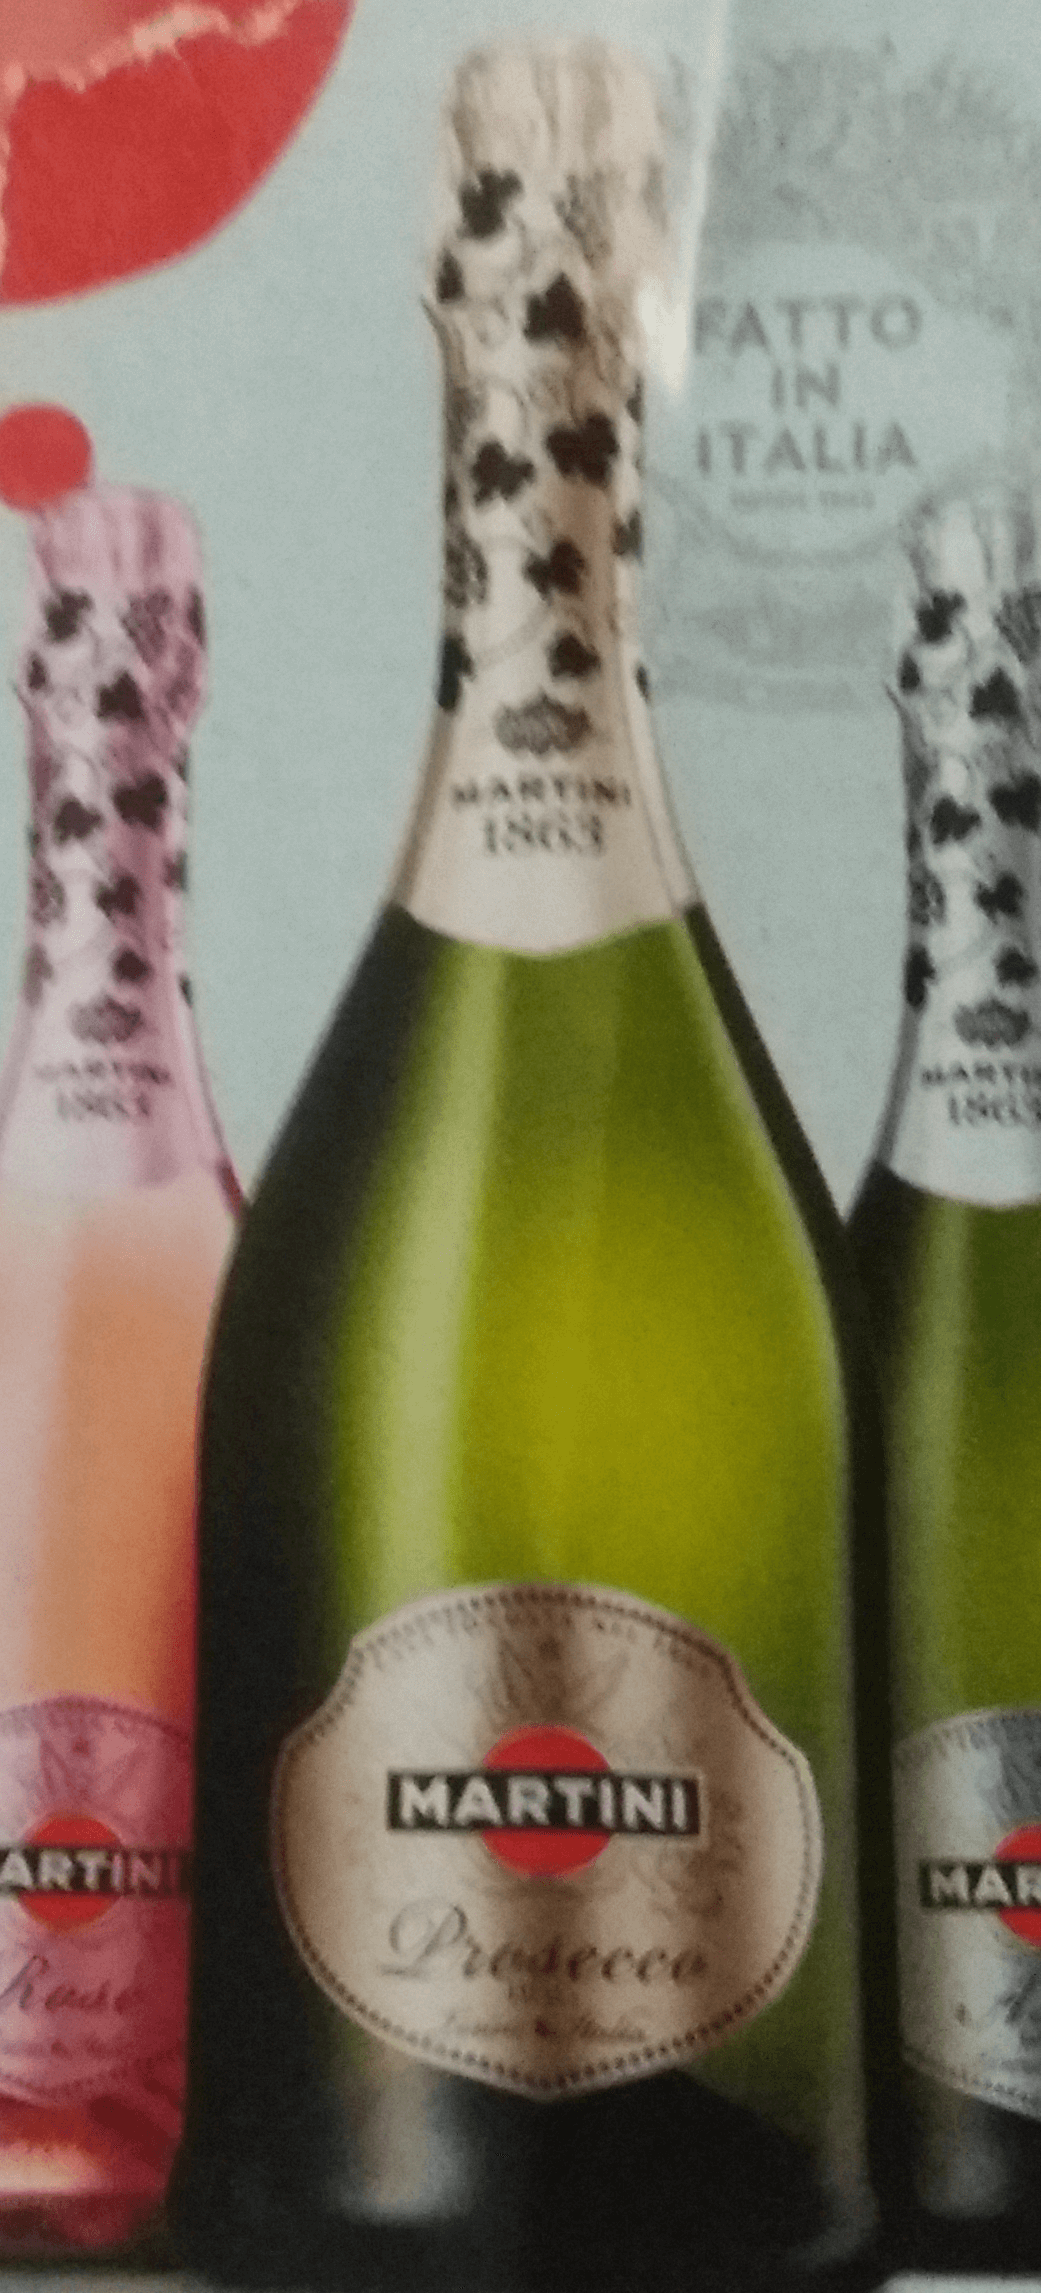
\includegraphics[width=20mm,height=20mm]{marcel2.png} & ``Una botella de champange representa celebración y diversión'' & ``Tener un título, se asocia a disfrutar placeres de la vida'' \\
\hline

3 & 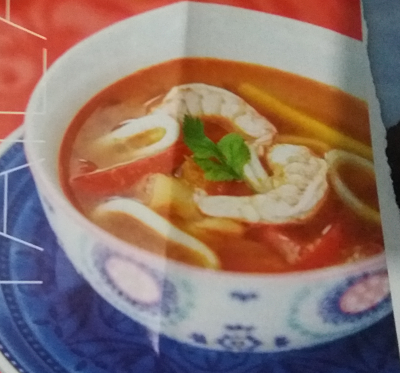
\includegraphics[width=20mm,height=20mm]{marcel3.png} & ``Un plato de comida especial representa los gustos exclusivos que uno se puede dar'' & ``Tener una buena situación económica'' \\
\hline

4 & 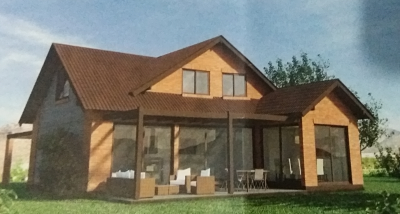
\includegraphics[width=20mm,height=20mm]{marcel5.png} & ``Tener una casa grande para la familia''  & ``El terminar una carrera implica tener un buen trabajo y mucho dinero, con el cual se puede optar a mejores condiciones de vida'' \\
\hline

5 & 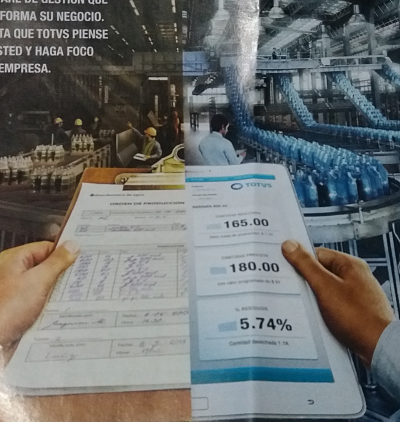
\includegraphics[width=20mm,height=20mm]{marcel6.png} & ``Participación activa en la industria'' & ``Generar aportes al trabajo, ser un buen profesional'' \\
\hline

6 & 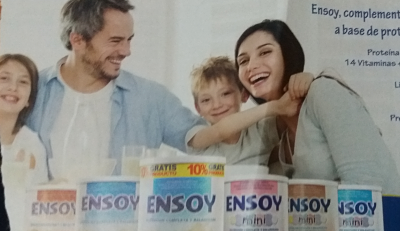
\includegraphics[width=20mm,height=20mm]{marcel7.png} & ``Tener una buena familia'' & ``Generar estabilidad y buenos lazos'' \\
\hline

7 & 
\includegraphics[width=20mm,height=20mm]{marcel8.png} & ``Dar la mano'' &  ``Generar buenos lazos profesionales y hacer negocios'' \\
\hline

\end{tabular}
\caption{Entrevista 1.}
\label{tabla:marcel}
\end{table}

Los grupos de imágenes que escogió el entrevistado fueron:\\

Grupo 1: imágenes 2 y 3, mencionando que son los placeres y gustos que se puede dar uno en la vida.\\

Grupo 2: imágenes 1, 4 y 6, mencionando el lado familiar, de tener algo consolidado y estable.\\

Grupo 3: imágenes 5 y 7, mencionando lado profesional, de tener estabilidad.\\

¿Cómo se ven afectadas tus motivaciones si desertas?.\\
``Los grupos 1 y 3 se complicarían ya que no se podrían lograr sin un título, en cambio el grupo 2 siempre estará porque es la familia''\\* 
\\
\\
\\
\\
\\
\\
\\
\\
\\
\\
\\
\\
\\
\\
\\*

\underline {ENTREVISTA 2} \\
Nombre: Fabián\\
Edad: 23\\
Carrera: 4to Año Ingeniería Civil Informática y Telecomunicaciones\\
Comuna: Puente Alto \\
\\
\begin{table}[H]
\centering
\begin{tabular}{>{\centering\arraybackslash}m{1cm} >{\centering\arraybackslash}m{2cm} >{\arraybackslash}m{5cm}>{\arraybackslash}m{5cm}}
\hline
Número  & Imagen & Descripción & Asociaciones \\
\hline \hline

1 & 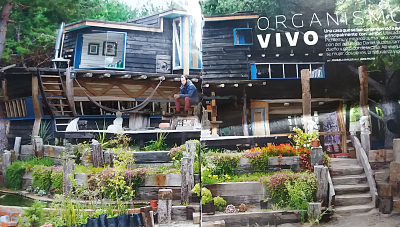
\includegraphics[width=20mm,height=20mm]{fabian1.png} & ``Casa grande'' &  ``Casa acogedora y armónica tanto para él como para su familia''\\
\hline

2 & 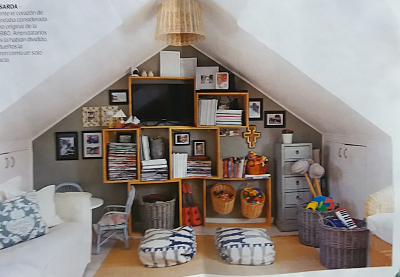
\includegraphics[width=20mm,height=20mm]{fabian2.png} & ``Diseño de espacio vanguardista y acogedor'' & ``Tener un espacio personal grande y vanguardista'' \\
\hline

3 & 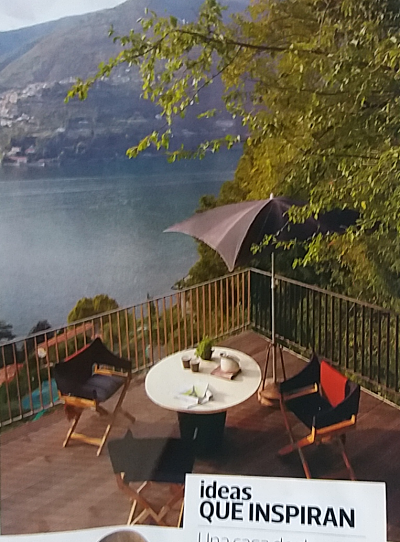
\includegraphics[width=20mm,height=20mm]{fabian3.png} & ``Casa en el lago'' & ``Espacio compartido, acogedor''\\
\hline

4 & 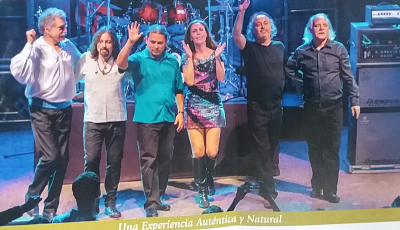
\includegraphics[width=20mm,height=20mm]{fabian4.png} & ``Cultura y música'' &  ``Tener una buena situación económica para disfrutar eventos culturales'' \\
\hline

5 & 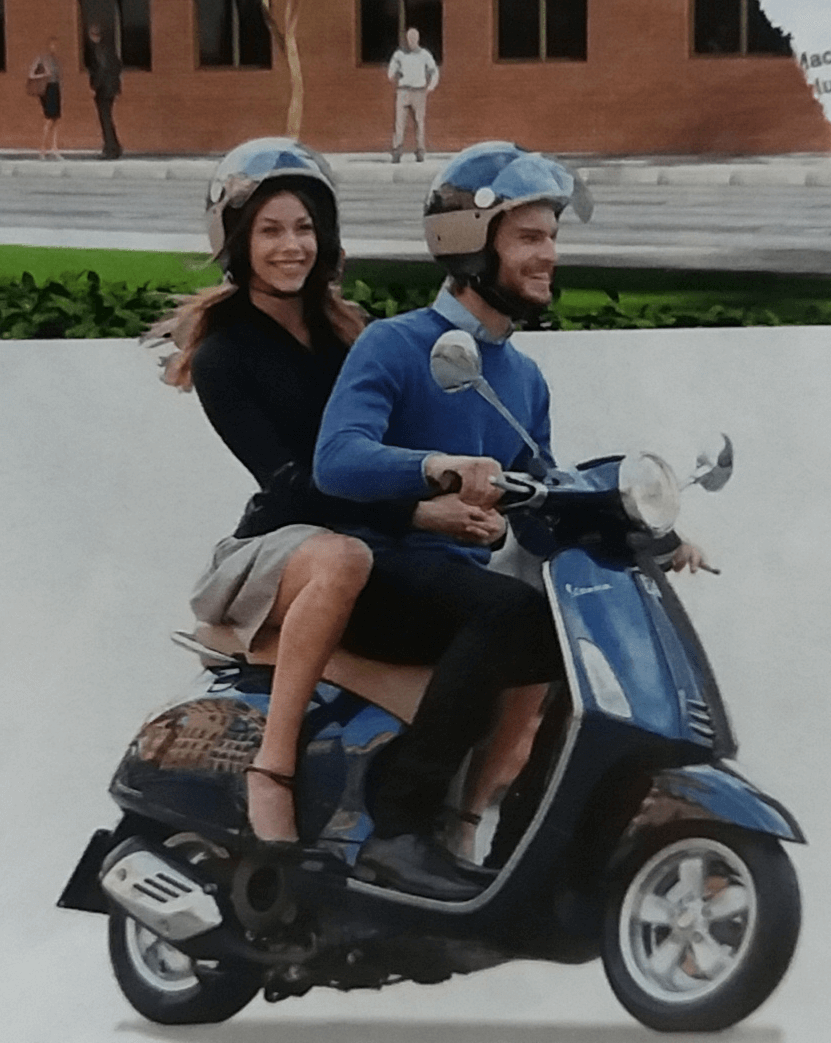
\includegraphics[width=20mm,height=20mm]{fabian5.png} & ``Pareja feliz'' & ``Compañera de vida bajo la premisa de familia, poder ofrecer un buen vivir a través de ser un profesional'' \\
\hline

6 & 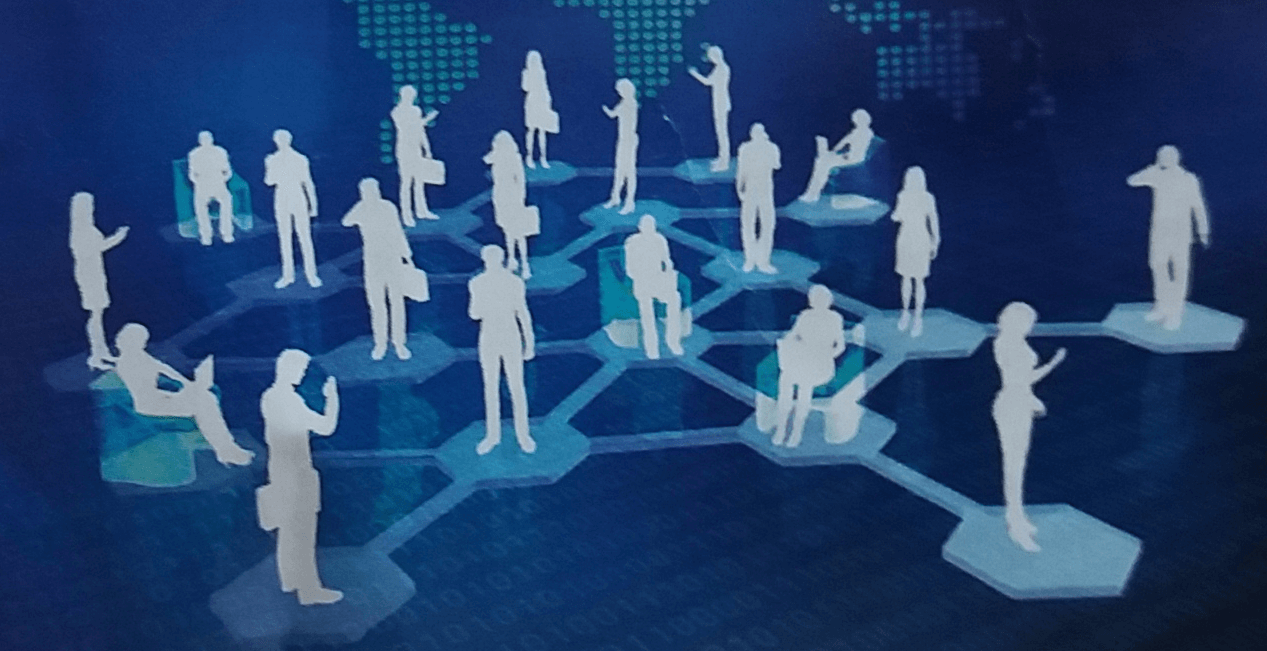
\includegraphics[width=20mm,height=20mm]{fabian6.png} & ``Redes profesionales'' & ``Generar proyectos de ingeniería''\\
\hline

7 & 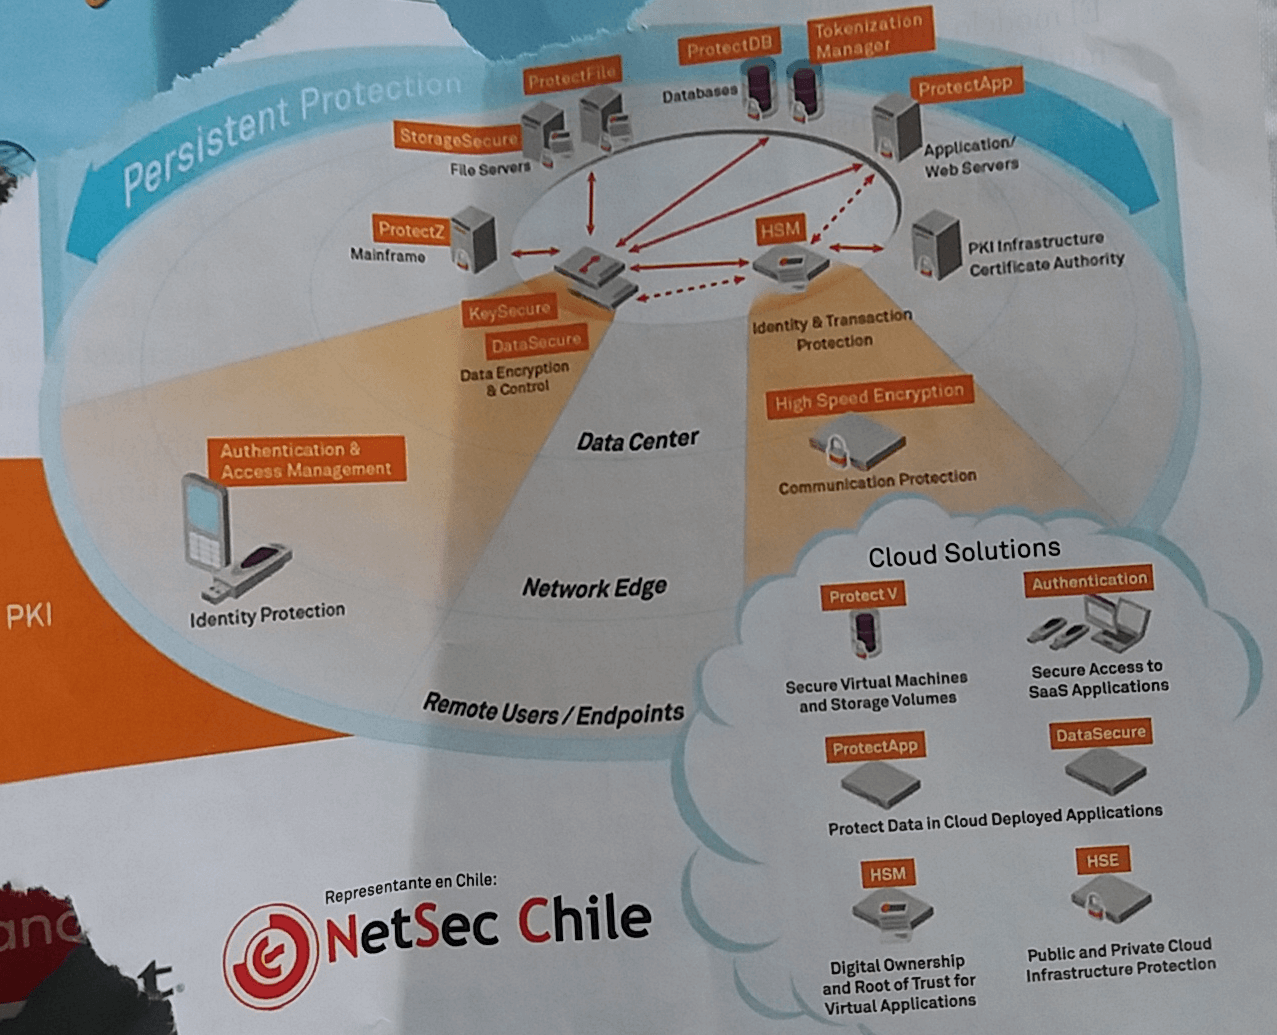
\includegraphics[width=20mm,height=20mm]{fabian7.png} & ``Redes informáticas''  & ``Tener un trabajo relacionado a redes informáticas y ser un buen profesional, para viajar por el mundo'' \\
\hline

8 & 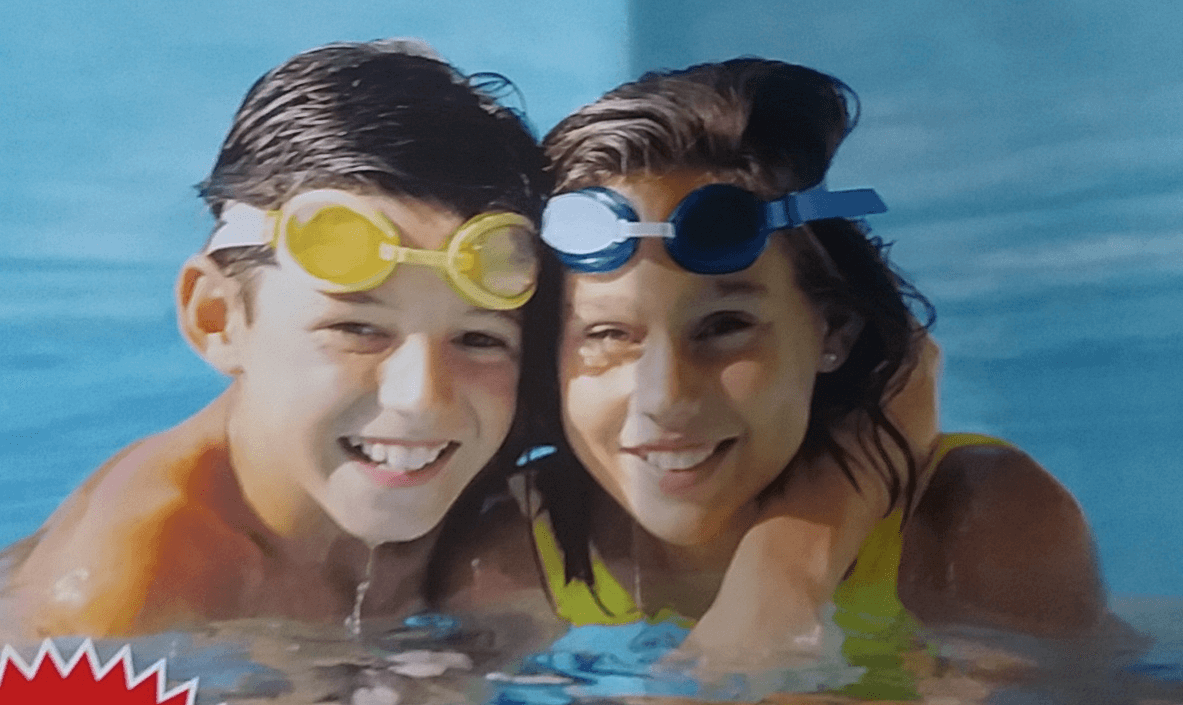
\includegraphics[width=20mm,height=20mm]{fabian8.png} & ``Niños felices'' & ``Sueños de ser papá, de tener las herramientas para dar un buen pasar'' \\
\hline

\end{tabular}
\caption{Entrevista 2.}
\label{tabla:fabian}
\end{table}



Los grupos de imágenes que escogió el entrevistado fueron:\\

Grupo 1: imágenes 4, 6 y 7, mencionando los gustos personales, ligando la parte profesional y la consecuencia de tener el dinero para darse los gustos.\\

Grupo 2: imágenes 5 y 8, mencionando la parte familiar.\\

Grupo 3: imágenes 1, 2, 3  mencionando la parte del hogar, una parte de acogida y en donde compartir.\\

¿Cómo se ven afectadas tus motivaciones si desertas?.\\

``Generaría mucha frustración, ya que la carrera es una herramienta para poder tener todo lo de las imágenes''\\
\\
\\
\\
\\
\\
\\
\\
\\
\\
\\
\\
\\
\\
\\
\\
\\
\\*

\underline {ENTREVISTA 3} \\* 
Nombre: Cristian\\
Edad: 25\\
Carrera: 5to Año Ingeniería Civil Informática y Telecomunicaciones\\
Comuna: La Florida\\

\begin{table}[H]
\centering
\begin{tabular}{>{\centering\arraybackslash}m{1cm} >{\centering\arraybackslash}m{2cm} >{\arraybackslash}m{5cm}>{\arraybackslash}m{5cm}}
\hline
Número  & Imagen & Descripción & Asociaciones \\
\hline \hline

1 & 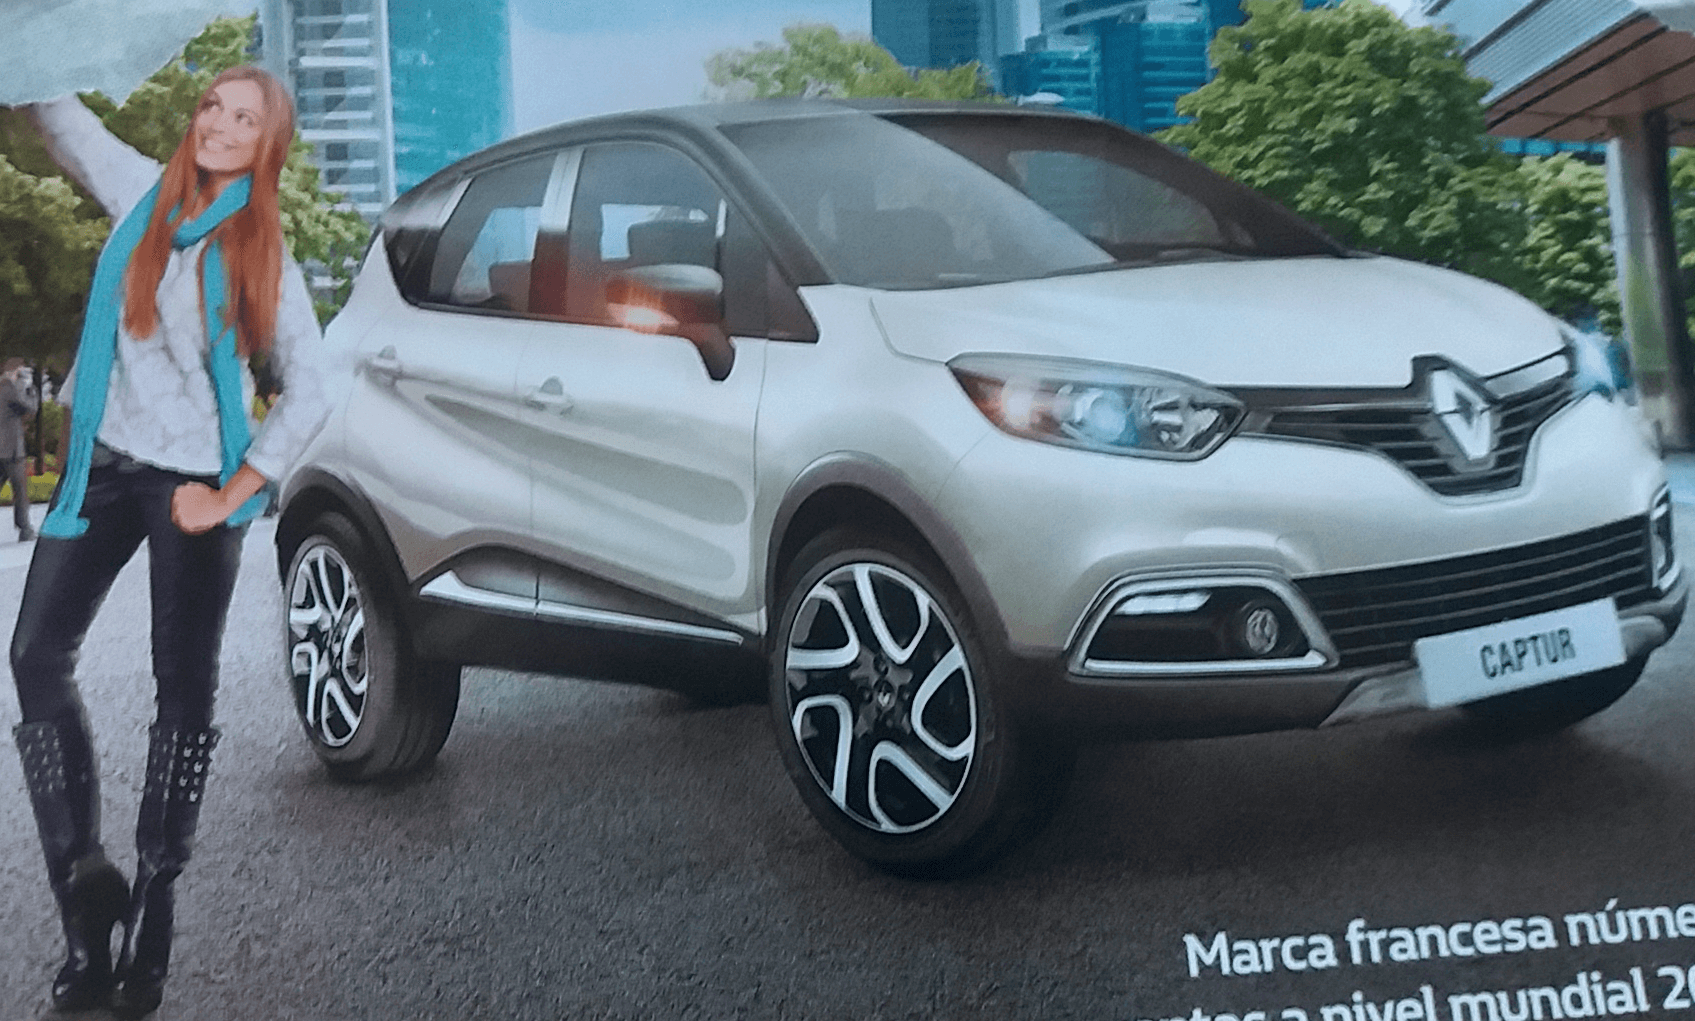
\includegraphics[width=20mm,height=20mm]{cristian1.png} & ``Auto'' & ``Tener un auto para tener independencia'' \\
\hline

2 & 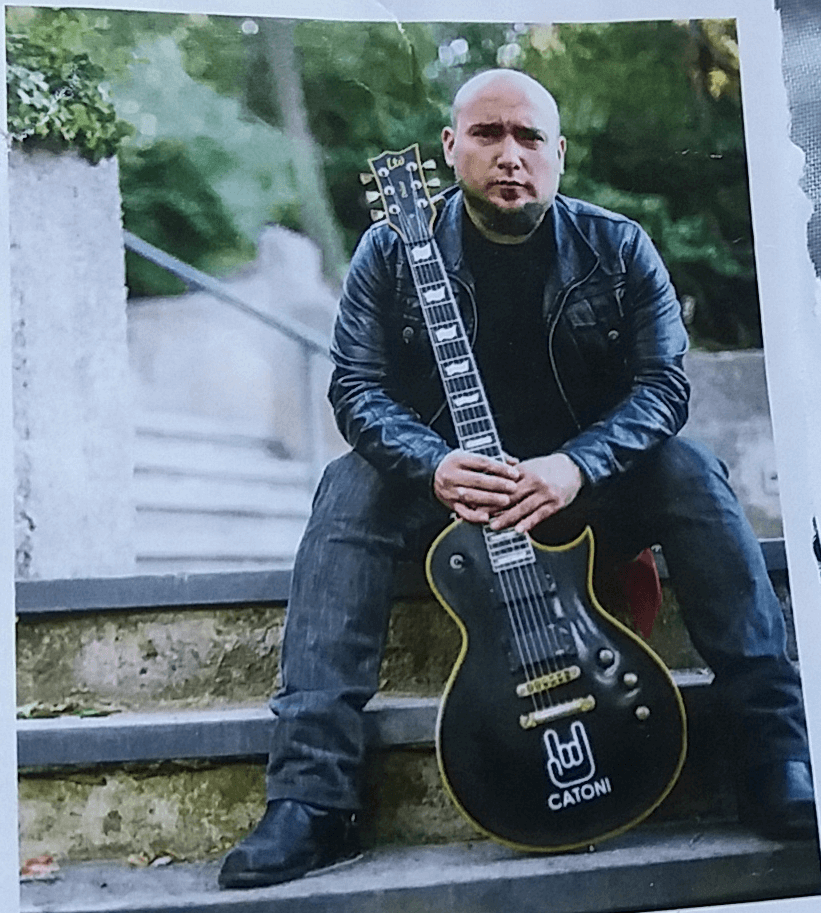
\includegraphics[width=20mm,height=20mm]{cristian2.png} & ``Guitarra'' & ``Tener sus gustos, la música'' \\
\hline

3 & 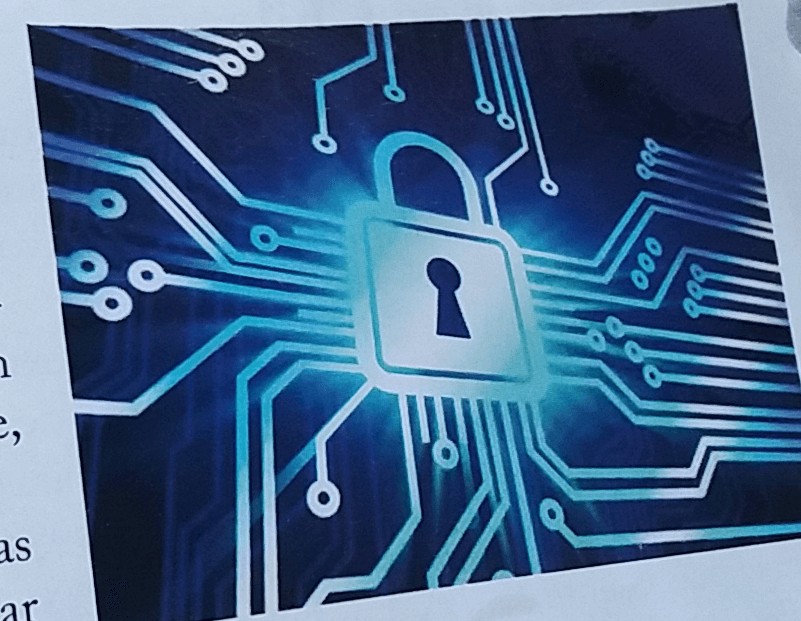
\includegraphics[width=20mm,height=20mm]{cristian3.png} & ``Seguridad informática'' & ``Poder dedicarse a la seguridad informática'' \\
\hline

4 & 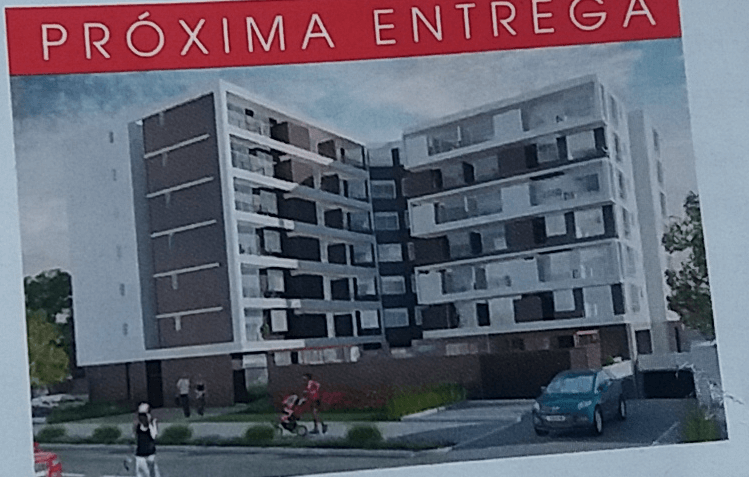
\includegraphics[width=20mm,height=20mm]{cristian4.png} & ``Departamentos'' & ``Tener un lugar donde vivir'' \\
\hline

5 & 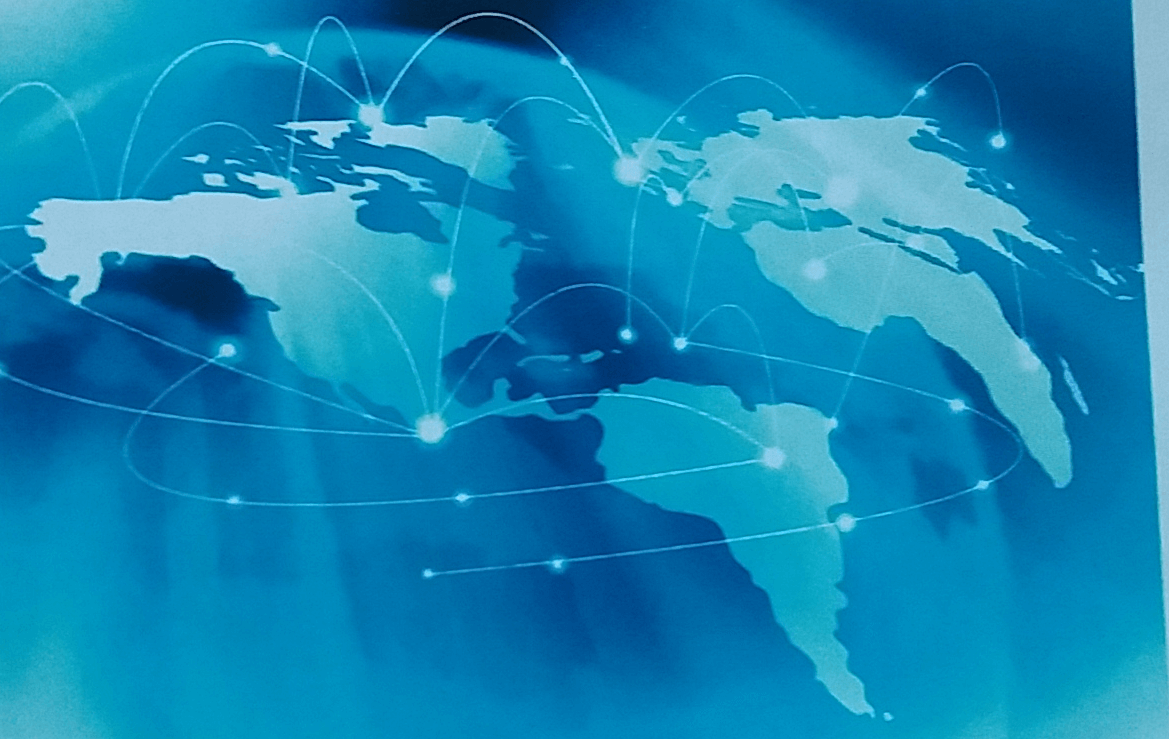
\includegraphics[width=20mm,height=20mm]{cristian5.png} & ``Mundo'' & ``Poder realizar viajes por el mundo''\\
\hline

6 & 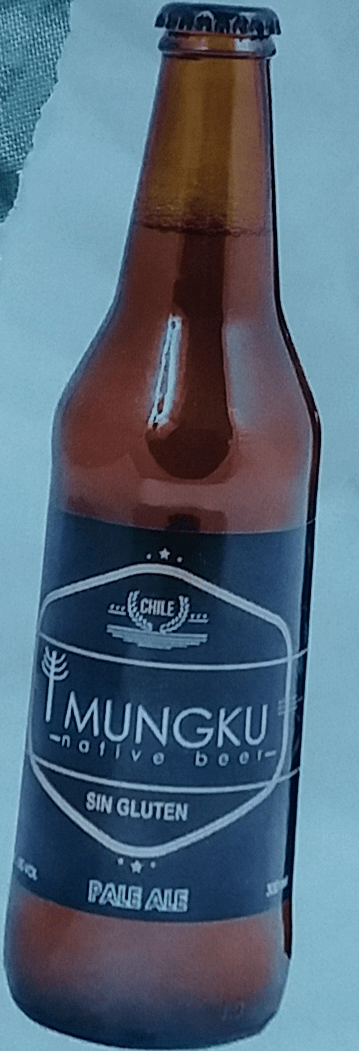
\includegraphics[width=20mm,height=20mm]{cristian6.png} & ``Cerveza'' & ``Poder darse sus gustos''\\
\hline

7 & 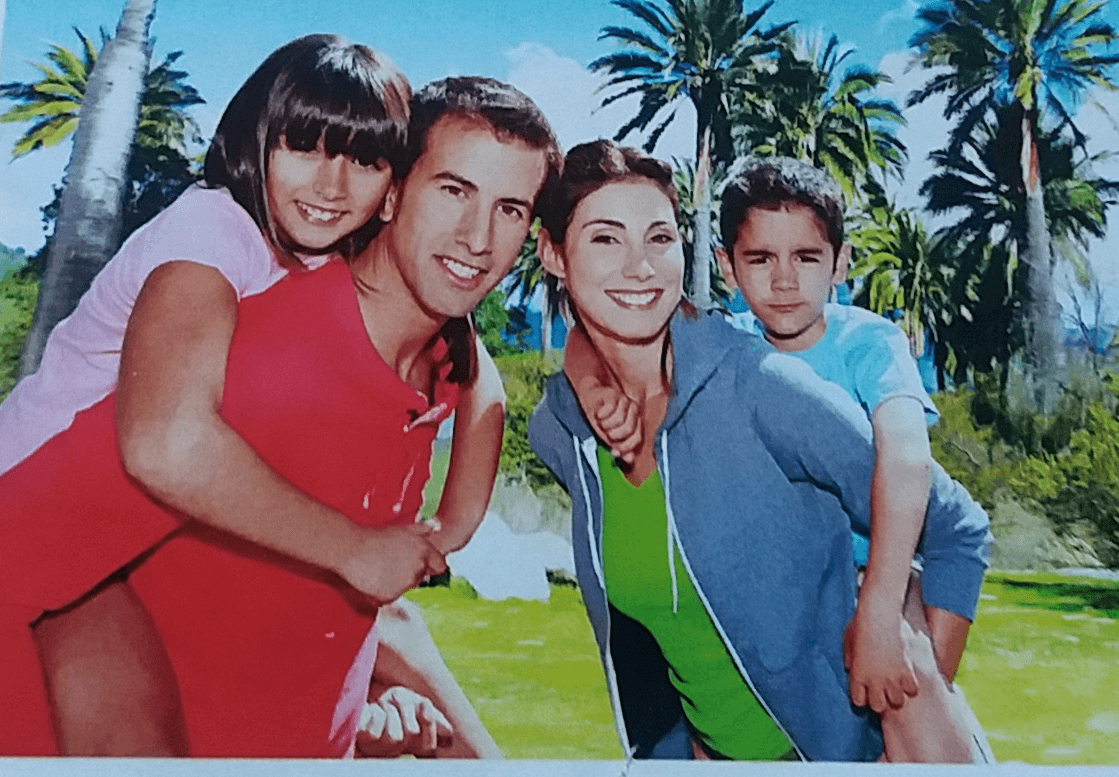
\includegraphics[width=20mm,height=20mm]{cristian7.png} & ``La familia'' & ``Tener una familia y tener plata para mantener a la familia'' \\
\hline

8 & 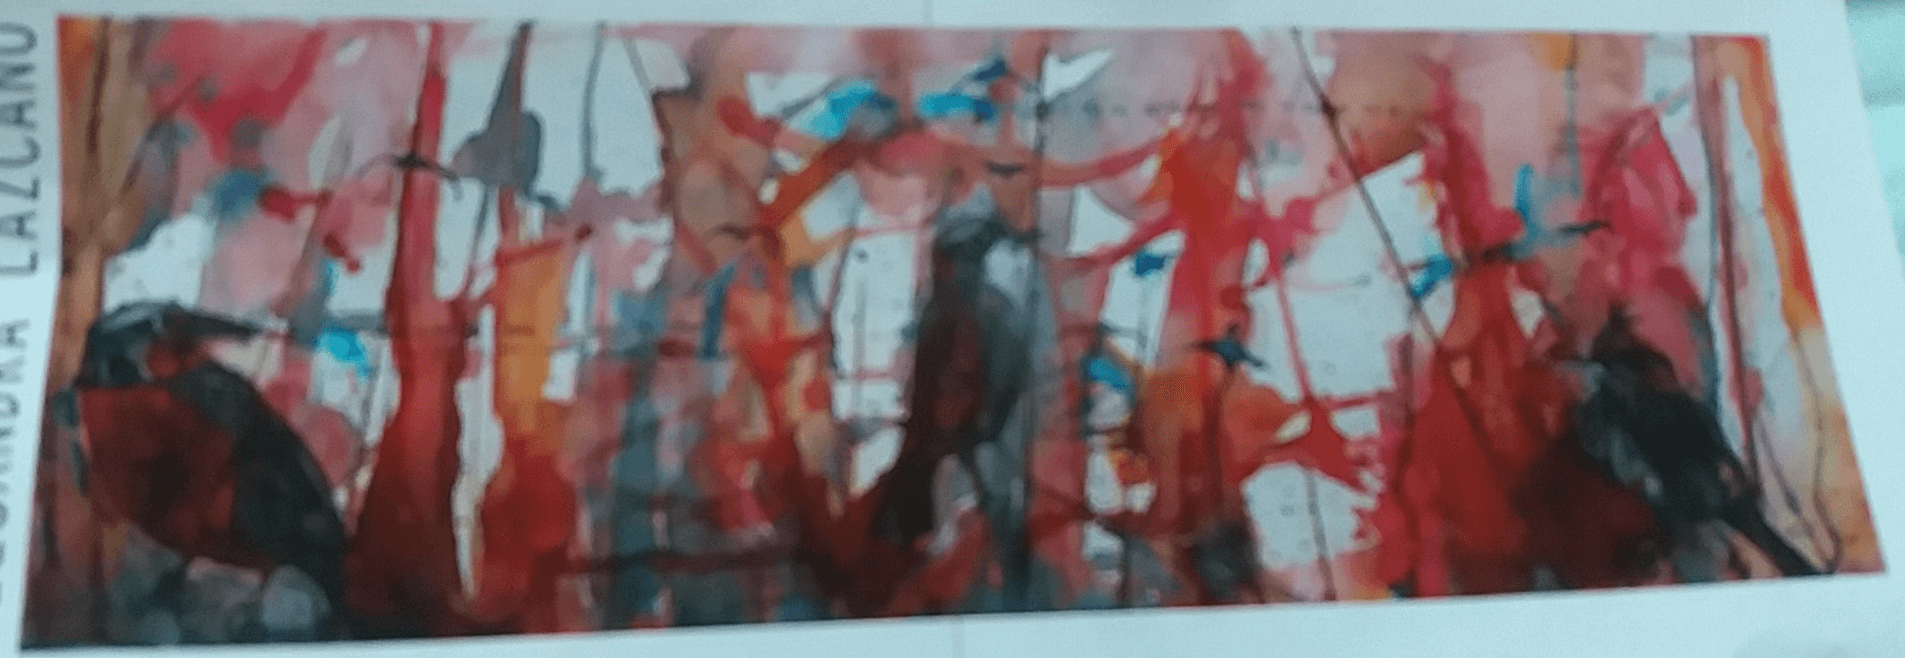
\includegraphics[width=20mm,height=20mm]{cristian8.png} & ``Decoración'' & ``Tener su casa decorada''\\
\hline

\end{tabular}
\caption{Entrevista 3.}
\label{tabla:cristian}
\end{table}

Los grupos de imágenes que escogió el entrevistado fueron:\\

Grupo 1: imágenes 1, 2 y 5, mencionando gustos personales, viajar a diferentes partes del mundo \\

Grupo 2: imágenes 3, 4 y 7, mencionando la parte familiar, trabajando en lo que le gusta, teniendo su casa y familia.\\

Grupo 3: imágenes 6 y 8, mencionando que son gustos exclusivos, no tan importantes como los del grupo 1.\\

¿Cómo se ven afectadas tus motivaciones si desertas?.\\

``Solamente podría tener la parte familiar, los otros grupos serían bastante complicados de satisfacer''\\
\newpage

\underline {ENTREVISTA 4} \\*
Nombre: Manuel\\
Edad: 24\\
Carrera: 4to Año Ingeniería Civil Informática y Telecomunicaciones\\
Comuna: Providencia\\

\begin{table}[H]
\centering
\begin{tabular}{>{\centering\arraybackslash}m{1cm} >{\centering\arraybackslash}m{2cm} >{\arraybackslash}m{5cm}>{\arraybackslash}m{5cm}}
\hline
Número & Imagen & Descripción & Asociaciones \\
\hline \hline

1 & 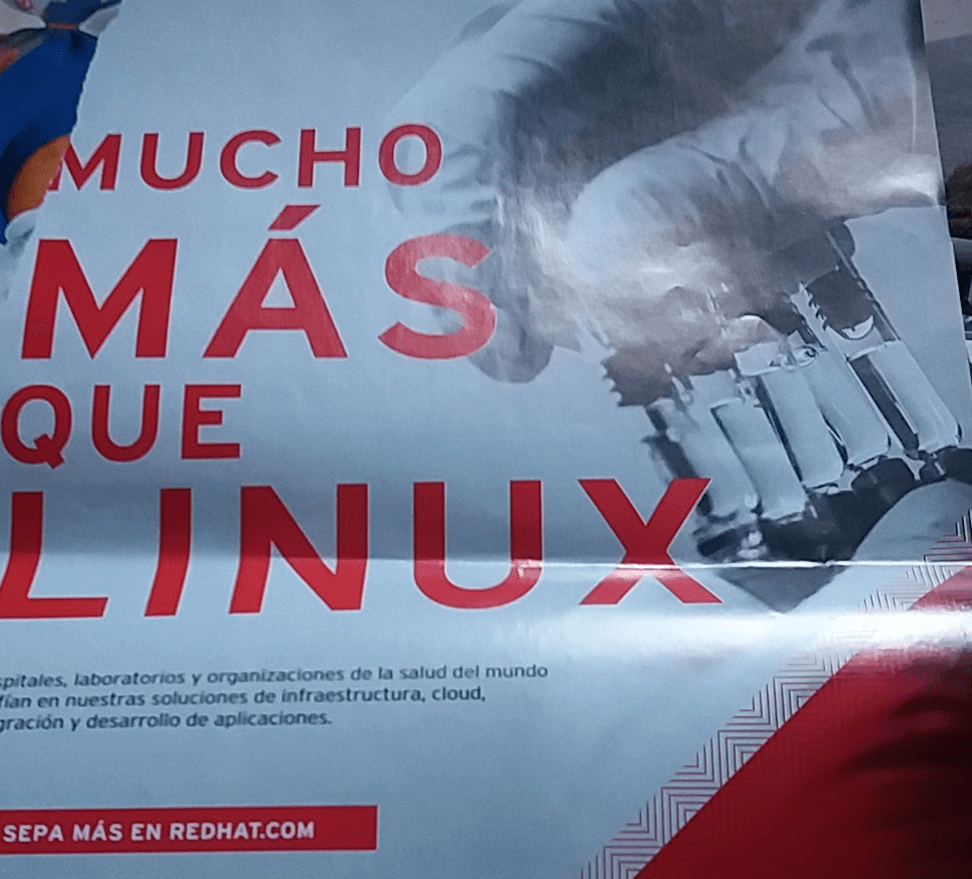
\includegraphics[width=20mm,height=20mm]{manuel1.png} & ``Linux'' & ``Tener sus trabajos realizados en Linux''\\
\hline

2 & 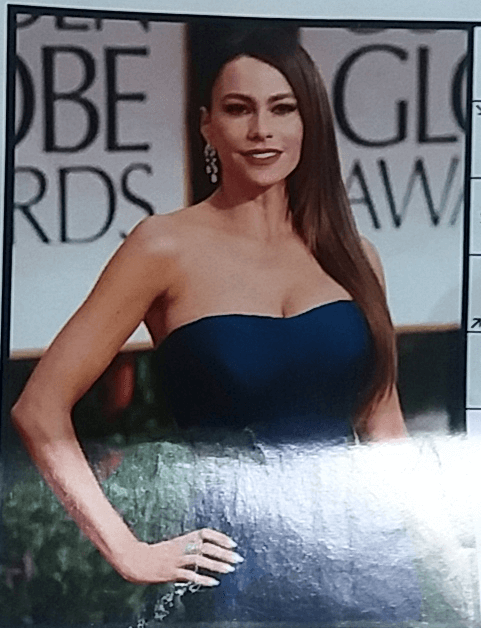
\includegraphics[width=20mm,height=20mm]{manuel2.png} & ``Mujer'' & ``Tener una linda mujer''\\
\hline

3 & 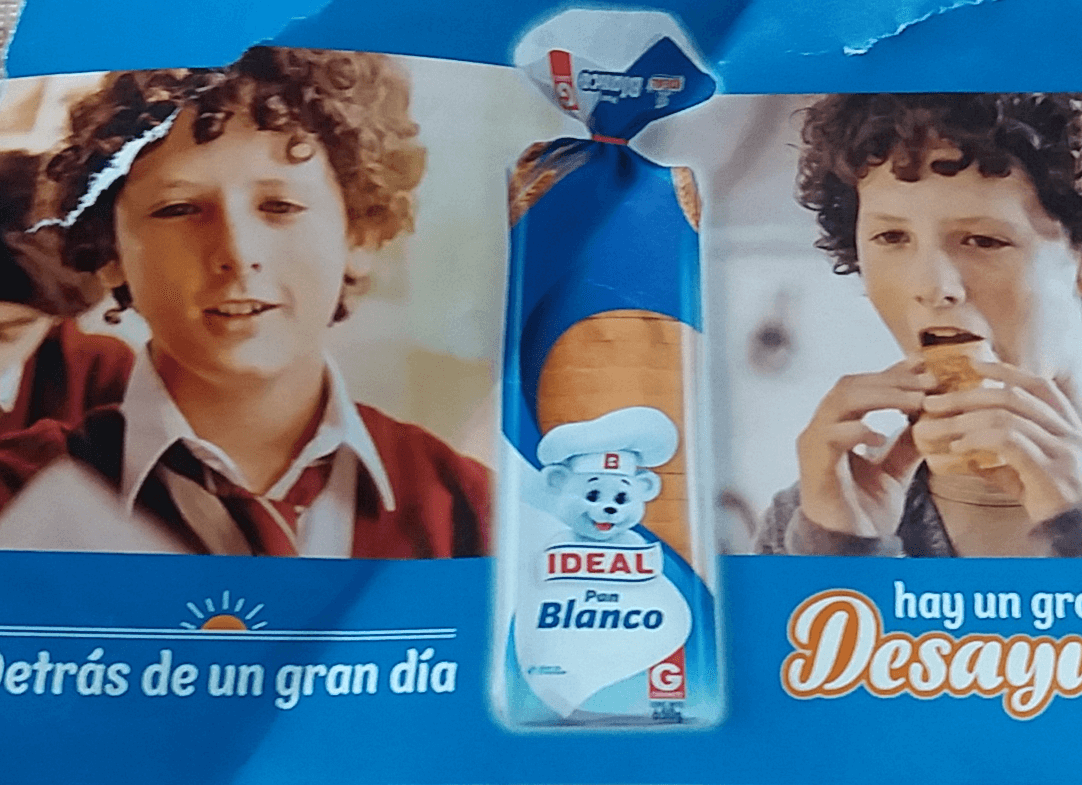
\includegraphics[width=20mm,height=20mm]{manuel3.png} & ``Pan'' & ``Tener para comer y una vida sana'' \\
\hline

4 & 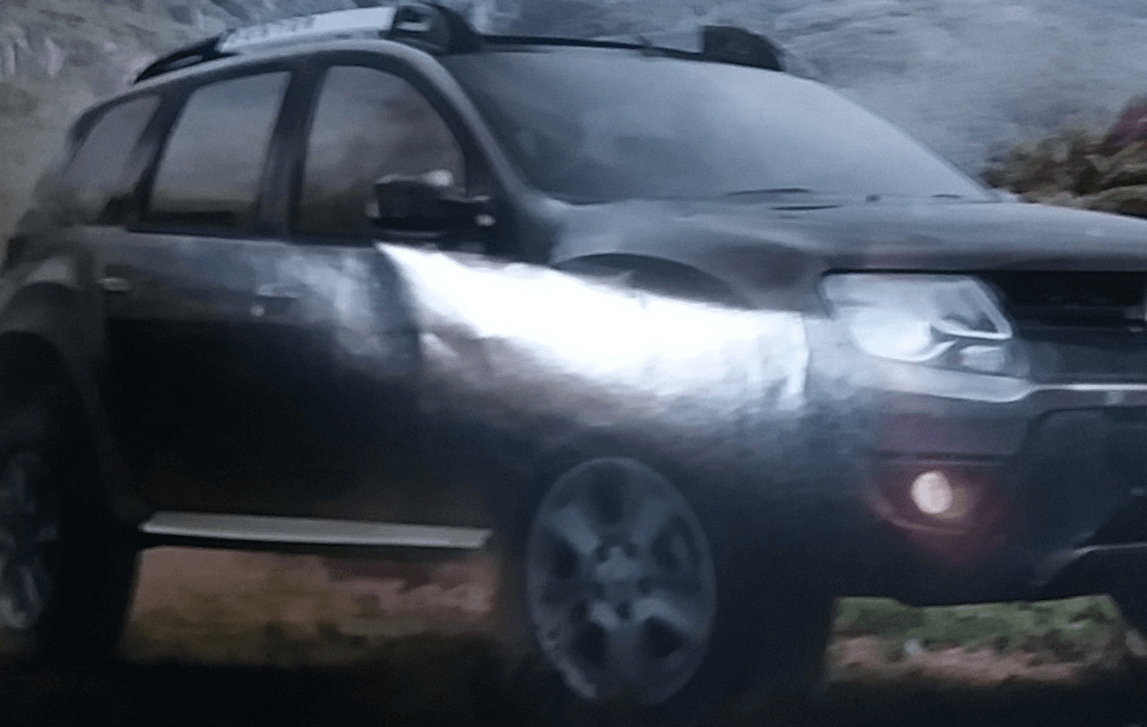
\includegraphics[width=20mm,height=20mm]{manuel4.png} & ``Auto'' & ``Tener suficiente trabajo para comprar un auto familiar'' \\
\hline

5 & 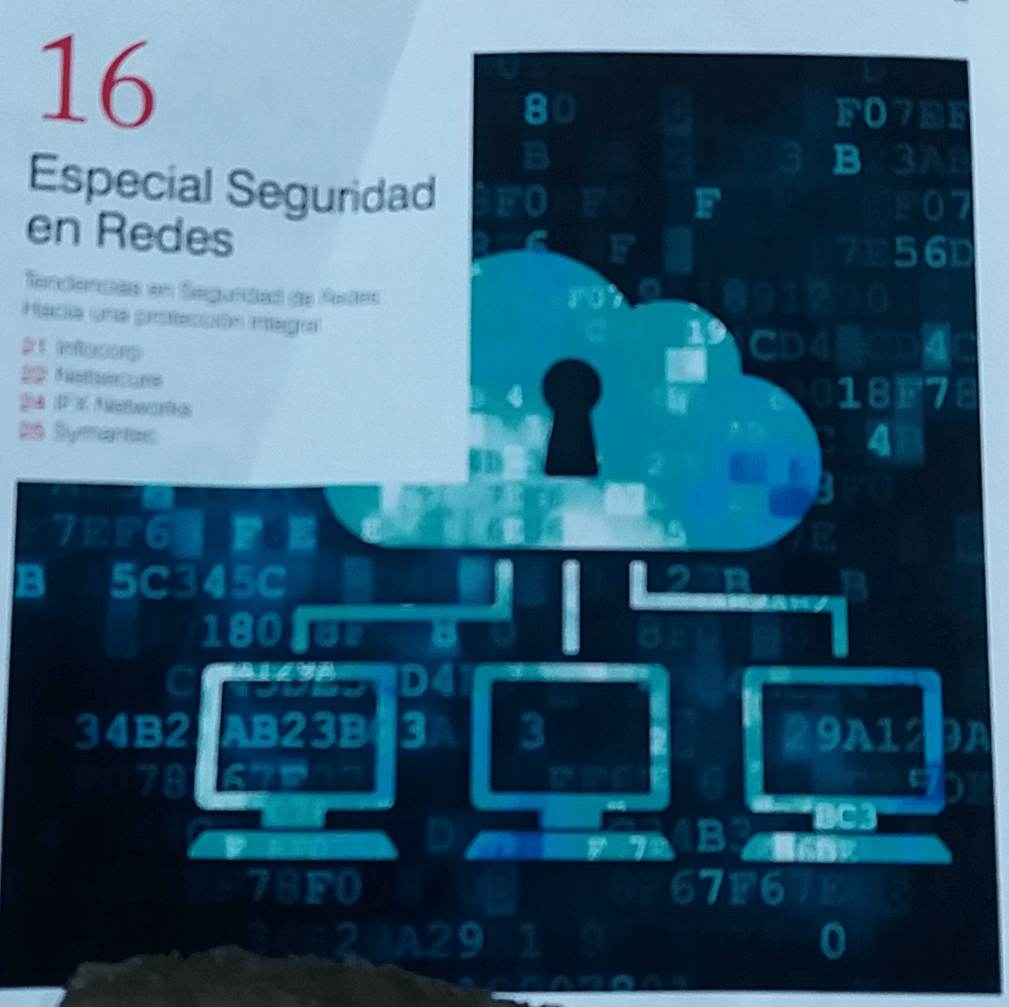
\includegraphics[width=20mm,height=20mm]{manuel5.png} & ``Redes informáticas'' & ``Tener un trabajo en el área de redes informáticas'' \\
\hline

6 & 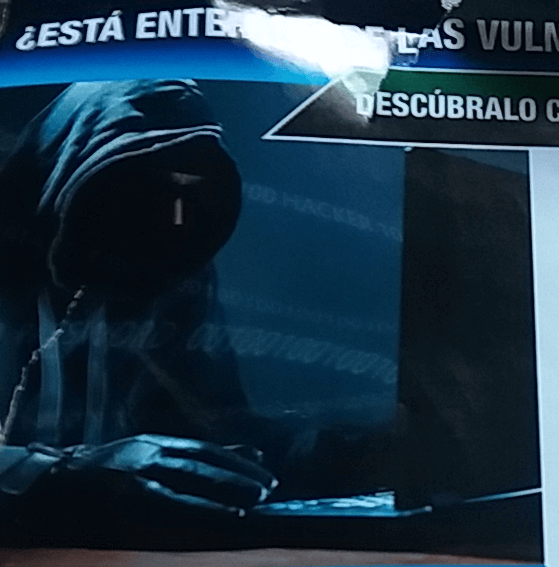
\includegraphics[width=20mm,height=20mm]{manuel6.png} & ``Seguridad informática'' & ``Poder desempeñarse en el área de seguridad informática'' \\
\hline

7 & 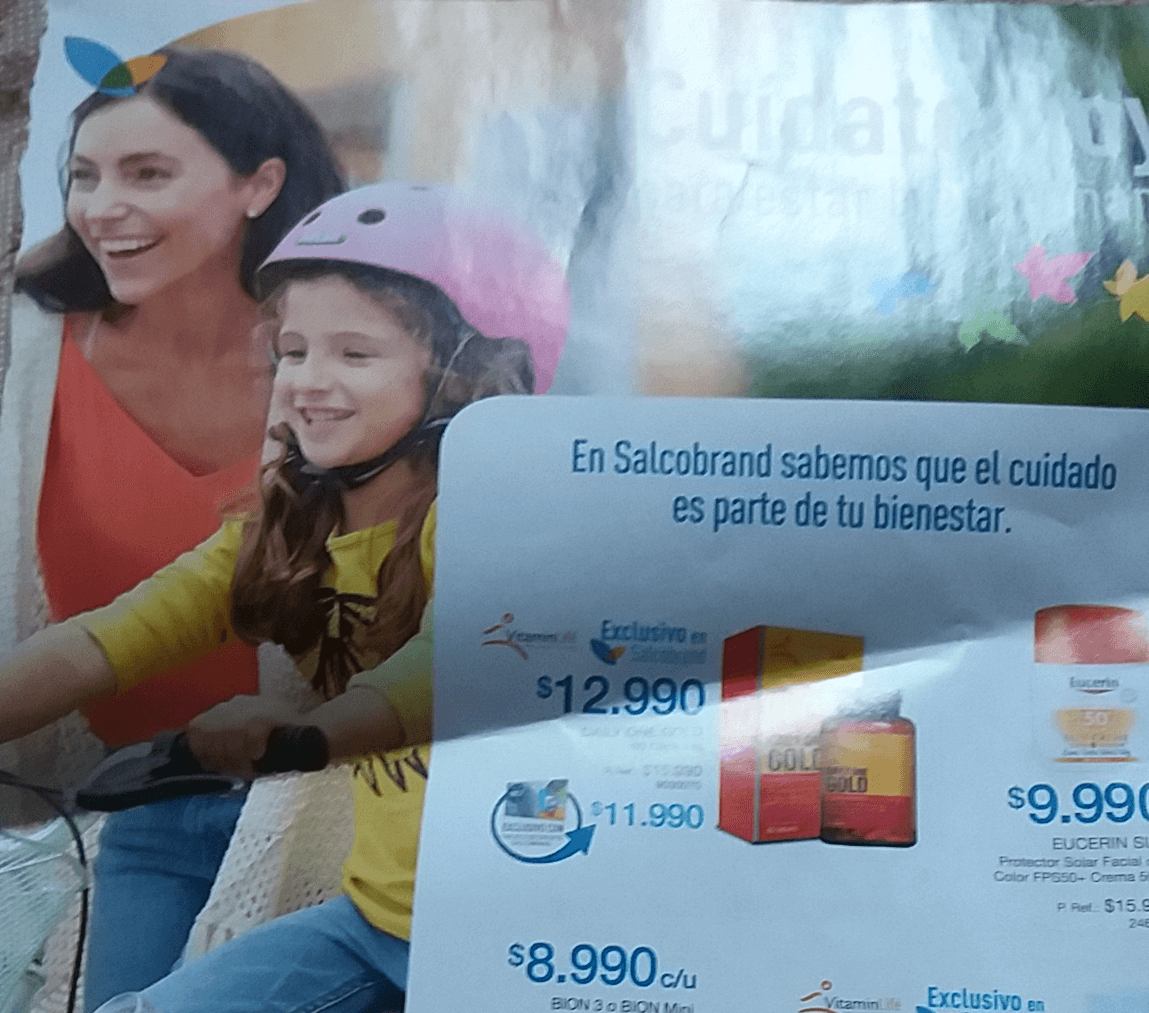
\includegraphics[width=20mm]{manuel7.png} & ``Madre e hija'' & ``Tener una familia con una hija sana'' \\
\hline

\end{tabular}
\caption{Entrevista 4.}
\label{tabla:manuel}
\end{table}

Los grupos de imágenes que escogió el entrevistado fueron:\\

Grupo 1: imágenes 2, 3, 4 y 7, mencionando que es la vida familiar. \\

Grupo 2: imágenes 1, 5 y 6 mencionando que es la vida trabajo.\\


¿Cómo se ven afectadas tus motivaciones si desertas?.\\

``No habría suficiente dinero para sustentar todo''\\

\newpage
\underline {ENTREVISTA 5} \\*
Nombre: Cristian\\
Edad: 23\\
Carrera: 4to Año Psicología\\
Comuna: Antofagasta\\

\begin{table}[H]
\centering
\begin{tabular}{>{\centering\arraybackslash}m{1cm} >{\centering\arraybackslash}m{2cm} >{\arraybackslash}m{5cm}>{\arraybackslash}m{5cm}}
\hline
Número  & Imagen & Descripción & Asociaciones \\
\hline \hline

1 & 
\includegraphics[width=20mm,height=20mm]{cristiant1.jpg} & ``Inexperto'' & ``Falta de experiencia al terminar la carrera, motiva a trabajar'' \\
\hline

2 & 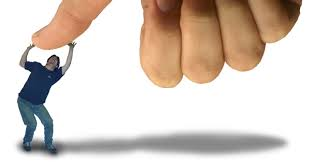
\includegraphics[width=20mm,height=20mm]{cristiant2.jpg} & ``Presión'' & ``Cerrar una etapa de la vida, para pasar a una siguiente'' \\
\hline

3 & 
\includegraphics[width=20mm,height=20mm]{cristiant3.jpg} & ``Profesional'' & ``Estar listo para enfrentar el mundo laboral'' \\
\hline

4 & 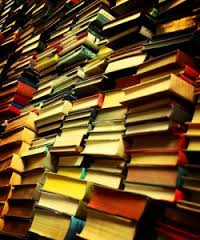
\includegraphics[width=20mm,height=20mm]{cristiant4.jpg} & ``Biblioteca'' & ``Dejar atrás los libros'' \\
\hline

5 & 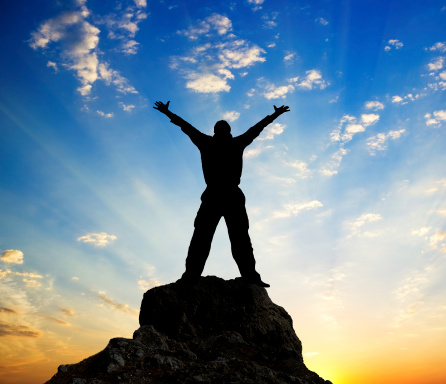
\includegraphics[width=20mm,height=20mm]{cristiant5.jpg} & ``Superación'' & ``Sentir la sensación de éxito''  \\
\hline

6 & 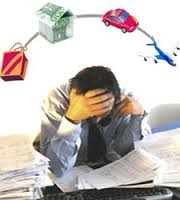
\includegraphics[width=20mm,height=20mm]{cristiant6.jpg} & ``Deudas'' & ``Tener mayores responsabilidades''\\
\hline

7 & \includegraphics[width=20mm,height=20mm]{cristiant7.jpg} & ``Magister'' & ``Poder sacar un postgrado'' \\
\hline

\end{tabular}
\caption{Entrevista 5.}
\label{tabla:cristiant}
\end{table}

Los grupos de imágenes que escogió el entrevistado fueron:\\

Grupo 1: imágenes 3, 4 y 5, mencionando que representa el éxito y el sentirse realizado por completar la carrera \\

Grupo 2: imágenes 1, 2, 6 y 7, mencionando la incertidumbre de enfrentar el mundo laboral.\\


¿Cómo se ven afectadas tus motivaciones si desertas?.\\

``Afectaría en la complicación de tener que pagar el crédito con aval del estado''\\

\newpage
\underline {ENTREVISTA 6}\\*
Nombre: Gabriel\\
Edad: 24\\
Carrera: 5to Año Psicología\\
Comuna: Santiago Centro\\

\begin{table}[H]
\centering
\begin{tabular}{>{\centering\arraybackslash}m{1cm} >{\centering\arraybackslash}m{2cm} >{\arraybackslash}m{5cm}>{\arraybackslash}m{5cm}}
\hline
Número  & Imagen & Descripción & Asociaciones \\
\hline \hline

1 & \includegraphics[width=20mm,height=20mm]{gabriel1.jpg} & ``Librero'' & ``Tener muchos libros por el gusto de leer'' \\
\hline

2 & \includegraphics[width=20mm,height=20mm]{gabriel2.jpg} & ``Psicología clínica'' & ``Dedicarse a su profesión'' \\
\hline

3 & \includegraphics[width=20mm,height=20mm]{gabriel3.jpg} & ``Graduado'' & ``Significa el cierre y el comienzo de una nueva etapa''`` \\
\hline

4 & \includegraphics[width=20mm,height=20mm]{gabriel4.jpg} & ``Autonomía'' & ``Ser una persona independiente'' \\
\hline

5 & \includegraphics[width=20mm,height=20mm]{gabriel5.jpg} & ``Deudas'' & ``Al titularse se tendrán muchas deudas'' \\
\hline

6 & \includegraphics[width=20mm,height=20mm]{gabriel6.jpg} & ``Profesor'' & ``Poder dar clases en un futuro''\\
\hline


\end{tabular}
\caption{Entrevista 6.}
\label{tabla:gabriel}
\end{table}

Los grupos de imágenes que escogió el entrevistado fueron:\\

Grupo 1: imágenes 1, 2, 3 y 6, mencionando que representa la independencia \\

Grupo 2: imágenes 4 y 5, mencionando que refleja el capitalismo y que siempre habrán deudas.\\


¿Cómo se ven afectadas tus motivaciones si desertas?.\\

``Afectaría en la complicación de tener independencia''\\

\newpage
\underline {ENTREVISTA 7}\\*
Nombre: Tania \\
Edad: 24\\
Carrera: 4to Año Ingeniería Civil Industrial \\
Comuna: Peñalolen \\

\begin{table}[H]
\centering
\begin{tabular}{>{\centering\arraybackslash}m{1cm} >{\centering\arraybackslash}m{2cm} >{\arraybackslash}m{5cm}>{\arraybackslash}m{5cm}}
\hline
Número  & Imagen & Descripción & Asociaciones \\
\hline \hline

1 & \includegraphics[width=20mm,height=20mm]{tania1.png} & ``Libertad laboral'' & ``Trabajar de forma independiente'' \\
\hline

2 & \includegraphics[width=20mm,height=20mm]{tania2.png} & ``Salud'' & ``Poder tener el dinero para obtener buenos tratamientos médicos'' \\
\hline

3 & \includegraphics[width=20mm,height=20mm]{tania3.png} & ``¿Qué hacer?'' & ``Necesidad de dinero y experiencia'' \\
\hline

4 & \includegraphics[width=20mm,height=20mm]{tania4.png} & ``Estilo de vida'' & ``Vida consciente con el planeta, a largo plazo'' \\
\hline

5 & \includegraphics[width=20mm,height=20mm]{tania5.png} & ``Seguridad'' & ``Desarrollar seguridad personal'' \\
\hline

6 & \includegraphics[width=20mm,height=20mm]{tania6.png} & ``Viajes'' & ``Tener la disponibilidad de tiempo y dinero, salir de la rutina, tener una vida más relajada''\\
\hline

7 & \includegraphics[width=20mm,height=20mm]{tania7.png} & ``Trabajo estable'' & ``Trabajar con personas, tener vida social''\\
\hline

\end{tabular}
\caption{Entrevista 7.}
\label{tabla:tania}
\end{table}

Los grupos de imágenes que escogió el entrevistado fueron:\\

Grupo 1: imágenes 1, 4 y 6, mencionando que representa tranquilidad y bienestar espiritual, relacionando el trabajo independiente que da libertad, complementándose con su estilo de vida y viajes.  \\

Grupo 2: imágenes 2 y 5, mencionando que representa seguridad, tener seguridad con su salud y frente a la delincuencia.\\

Grupo 3: imágenes 3 y 7, mencionando que representa el ámbito laboral, el no saber en que trabajará, pero si tener una idea de que trabajará con un grupo de gente y hacer vida social.\\

¿Cómo se ven afectadas tus motivaciones si desertas?.\\

``Solo se verían cumplidas las imágenes del grupo 1 y muy a largo plazo, los otros grupos no los podría cumplir''

\newpage
\underline {ENTREVISTA 8}\\*
Nombre: Carlos\\
Edad: 22 \\
Carrera: 3er Año Ingeniería Comercial\\
Comuna: Santiago Centro\\

\begin{table}[H]
\centering
\begin{tabular}{>{\centering\arraybackslash}m{1cm} >{\centering\arraybackslash}m{2cm} >{\arraybackslash}m{5cm}>{\arraybackslash}m{5cm}}
\hline
Número  & Imagen & Descripción & Asociaciones \\
\hline \hline

1 & \includegraphics[width=20mm,height=20mm]{carlos1.png} & ``Tranquilidad'' & ``Terminar una carrera transmite seguridad y sentirse útil para algo'' \\
\hline

2 & \includegraphics[width=20mm,height=20mm]{carlos2.png} & ``Presentación de Apple'' & ``Representa el triunfo que puede llegar a tener como profesional.'' \\
\hline

3 & \includegraphics[width=20mm,height=20mm]{carlos3.png} & ``Triunfo''' & ``Reconocimiento por llegar a una meta'' \\
\hline

4 & \includegraphics[width=20mm,height=20mm]{carlos4.png} & ``Tiempo libre'' & ``Expresa los pasatiempos que se pueden realizar al terminar la carrera'' \\
\hline

5 & \includegraphics[width=20mm,height=20mm]{carlos5.png} & ``Pasatiempos'' & ``Poder tener la libertad de darse tiempos libres y hacer las cosas que uno quiere'' \\
\hline

6 & \includegraphics[width=20mm,height=20mm]{carlos6.png} & ``Trabajo'' & ``Trabajar de forma relajada, ya que con el título tienes una base para dedicarse a lo que te gusta'' \\
\hline


\end{tabular}
\caption{Entrevista 8.}
\label{tabla:carlos}
\end{table}

Los grupos de imágenes que escogió el entrevistado fueron:\\
\\
\\*

Grupo 1: imágenes 1, 4 y 5, mencionando que representa el tiempo libre, que ya obtenido un título, ya tienes una base para poder tener dinero y dedicarse a gustos más caros. \\

Grupo 2: imágenes 2, 3 y 6, mencionando que representa el triunfo, el éxito de terminar una meta.\\


¿Cómo se ven afectadas tus motivaciones si desertas?.\\

``En lo personal tener un título no es el único camino para cumplir mis sueños, la sociedad impone que debe ser así, pero yo no lo veo como la única opción.''

\newpage
\underline {ENTREVISTA 9}\\*
Nombre: Ilana\\
Edad: 23\\
Carrera: 3er Año Ingeniería Comercial\\
Comuna: Las Condes \\

\begin{table}[H]
\centering
\begin{tabular}{>{\centering\arraybackslash}m{1cm} >{\centering\arraybackslash}m{2cm} >{\arraybackslash}m{5cm}>{\arraybackslash}m{5cm}}
\hline
Número  & Imagen & Descripción & Asociaciones \\
\hline \hline

1 & \includegraphics[width=20mm,height=20mm]{ilana1.png} & ``Comida'' & ``Dedicar tiempo para mi persona y realizar lo que me gusta, la cocina.'' \\
\hline

2 & \includegraphics[width=20mm,height=20mm]{ilana2.png} & ``Curso de inglés'' & ``Tener tiempo para poder realizar un curso de inglés y viajar al extranjero.'' \\
\hline

3 & \includegraphics[width=20mm,height=20mm]{ilana3.png} & ``Libertad'' & ``Terminar la carrera, da una sensación de libertad y triunfo.'' \\
\hline

4 & \includegraphics[width=20mm,height=20mm]{ilana4.png} & ``Viajes'' & ``Después de la carrera hay tiempo para disfrutar y conocer el mundo.'' \\
\hline

5 & \includegraphics[width=20mm,height=20mm]{ilana5.png} & ``Independencia'' & ``Poder vivir sola y tener mi departamento.'' \\
\hline

6 & \includegraphics[width=20mm,height=20mm]{ilana6.png} & ``Trabajo'' & ``Encontrar un trabajo en una empresa prestigiosa.'' \\
\hline


\end{tabular}
\caption{Entrevista 9.}
\label{tabla:ilana}
\end{table}

Los grupos de imágenes que escogió el entrevistado fueron:\\

Grupo 1: imágenes 1 y 3, mencionando que representa el relajo y el poder realizar sus gustos, como cocinar. \\

Grupo 2: imágenes 2 y 4, mencionando que representa los viajes, y que aprender un idioma nuevo abre las puertas a conocer otros lugares.\\

Grupo 3: imágenes 5 y 6, mencionado que representa su independencia, para poder tener su departamento, necesita de un trabajo.\\


¿Cómo se ven afectadas tus motivaciones si desertas?.\\

``Seria difícil cumplir el grupo 3, no podría hacer el grupo 2, solamente me podría dedicar a las imágenes del grupo 1.'' \\
\\
\\
\\
\\
\\
\\
\\
\\
\\
\\
\\
\\
\\
\\
\\
\\
\\*

\underline {ENTREVISTA 10}\\*
Nombre: Oscar\\
Edad: 28\\
Carrera: 6to Año Ingeniería Civil en Informática y Telecomunicaciones \\
Comuna: Macul \\

\begin{table}[H]
\centering
\begin{tabular}{>{\centering\arraybackslash}m{1cm} >{\centering\arraybackslash}m{2cm} >{\arraybackslash}m{5cm}>{\arraybackslash}m{5cm}}
\hline
Número  & Imagen & Descripción & Asociaciones \\
\hline \hline

1 & \includegraphics[width=20mm,height=20mm]{oscar1.png} & ``Scooter'' & ``Representa el vehículo que podría adquirir teniendo recursos'' \\
\hline

2 & \includegraphics[width=20mm,height=20mm]{oscar2.png} & ``Departamento'' & ``Representa la adquisición de un bien raíz gracias al trabajo después de títulado'' \\
\hline

3 & \includegraphics[width=20mm,height=20mm]{oscar3.png} & ``Aire acondicionado'' & ``Representa las comodidades que uno podría tener una vez trabajando'' \\
\hline

4 & \includegraphics[width=20mm,height=20mm]{oscar4.png} & ``Plato de comida'' & ``Representa los gustos que me podría dar, teniendo recursos.'' \\
\hline

5 & \includegraphics[width=20mm,height=20mm]{oscar5.png} & ``Buda'' & ``Representa crecimiento personal y laboral'' \\
\hline

6 & \includegraphics[width=20mm,height=20mm]{oscar6.png} & ``Descanso'' & ``Representa los viajes, los gustos, el relajo que podría tener'' \\
\hline

7 & \includegraphics[width=20mm,height=20mm]{oscar7.png} & ``Arte'' & ``Representa al parte artística que podría dedicarme teniendo recursos'' \\
\hline

8 & \includegraphics[width=20mm,height=20mm]{oscar8.png} & ``Viajes'' & ``Representa los lugares que podría conocer'' \\
\hline

\end{tabular}
\caption{Entrevista 10.}
\label{tabla:oscar}
\end{table}

Los grupos de imágenes que escogió el entrevistado fueron:\\

Grupo 1: imágenes 2, 3 y 6, mencionando que representa su parte hogar. \\

Grupo 2: imagen 4, mencionando que representa sus gustos.\\

Grupo 3: imágenes 1, 5, 7 y 8, mencionando que representa su parte personal, sus sueños como persona. \\

¿Cómo se ven afectadas tus motivaciones si desertas?.\\

``Para cumplir todo esto, se necesitan recursos, y en el fondo la carrera me da un pie laboral para tener una buena situación económica, sin recursos se vería todo frustrado.'' \\

\newpage
\underline {ENTREVISTA 11}\\*
Nombre: Diego\\
Edad: 20\\
Carrera: 2do Año Ingeniería Civil Industrial\\
Comuna: Quinta Normal\\

\begin{table}[H]
\centering
\begin{tabular}{>{\centering\arraybackslash}m{1cm} >{\centering\arraybackslash}m{2cm} >{\arraybackslash}m{5cm}>{\arraybackslash}m{5cm}}
\hline
Número  & Imagen & Descripción & Asociaciones \\
\hline \hline

1 & \includegraphics[width=20mm,height=20mm]{diego1.png} & ``Gustos'' & ``Poder obtener gustos exclusivos gracias al dinero.'' \\
\hline

2 & \includegraphics[width=20mm,height=20mm]{diego2.png} & ``Hogar'' & ``Poder conseguir un buen hogar a partir del dinero'' \\
\hline

3 & \includegraphics[width=20mm,height=20mm]{diego3.png} & ``Empresario'' & ``Es a lo que uno aspira ser como ingeniero, teniendo buen puesto y reputación.'' \\
\hline

4 & \includegraphics[width=20mm,height=20mm]{diego4.png} & ``Superación personal'' & ``Es el logro de cumplir con el objetivo de ser ingeniero'' \\
\hline

5 & \includegraphics[width=20mm,height=20mm]{diego5.png} & ``Pareja'' & ``Felicidad y estabilidad amorosa, gracias a una buena situación económica.'' \\
\hline

6 & \includegraphics[width=20mm,height=20mm]{diego6.png} & ``Música'' & ``Cumplir con el sueño de ser músico una vez teniendo estabilidad economica'' \\
\hline

7 & \includegraphics[width=20mm,height=20mm]{diego7.png} & ``Viajes'' & ``Sin dinero no se puede viajar, y teniendo una carrera, uno puede ganar mucho dinero.'' \\
\hline

\end{tabular}
\caption{Entrevista 11.}
\label{tabla:diego}
\end{table}

Los grupos de imágenes que escogió el entrevistado fueron:\\

Grupo 1: imágenes 3 y 4, mencionando que representa el  trabajo donde señala que es su aspiración a ser y su logro personal\\

Grupo 2: imágenes 2 y 5, mencionando que representa la familia, donde espera una relación de pareja y el hogar\\

Grupo 3: imágenes 1, 6 y 7, mencionando que representa sus gustos personales.\\

¿Cómo se ven afectadas tus motivaciones si desertas?.\\

``No se podría conseguir el grupo 2 por falta de dinero al igual que el grupo 3, y el grupo 1 se vería frustrado, por el punto de que quiero ser ingeniero.'' \\
\\
\\
\\
\\
\\
\\
\\
\\
\\
\\
\\
\\
\\
\\*
\underline {ENTREVISTA 12}\\*
Nombre: Matias\\
Edad: 21\\
Carrera: 2do Año Ingeniería Civil Industrial\\
Comuna: Rancagua\\

\begin{table}[H]
\centering
\begin{tabular}{>{\centering\arraybackslash}m{1cm} >{\centering\arraybackslash}m{2cm} >{\arraybackslash}m{5cm}>{\arraybackslash}m{5cm}}
\hline
Número  & Imagen & Descripción & Asociaciones \\
\hline \hline

1 & \includegraphics[width=20mm,height=20mm]{matias1.png} & ``Gustos'' & ``Tener un sueldo millonario para disfrutar de los gustos'' \\
\hline

2 & \includegraphics[width=20mm,height=20mm]{matias2.png} & ``Familia'' & ``Ser solvente'' \\
\hline

3 & \includegraphics[width=20mm,height=20mm]{matias3.png} & ``Departamento'' & ``Tener la autonomía de vivir solo y tener un hogar'' \\
\hline

4 & \includegraphics[width=20mm,height=20mm]{matias4.png} & ``Pasatiempos'' & ``Con un titulo se puede obtener mucha plata y con ella poder tener pasatiempos'' \\
\hline

5 & \includegraphics[width=20mm,height=20mm]{matias5.png} & ``Placeres'' & ``Comprar cosas exclusivas'' \\
\hline

6 & \includegraphics[width=20mm,height=20mm]{matias6.png} & ``Reconocimiento'' & ``Estar graduado y ser reconocido como un ingeniero.'' \\
\hline

7 & \includegraphics[width=20mm,height=20mm]{matias7.png} & ``Grupo de empresarios'' & ``Es lo que quiero llegar hacer, y tener un trabajo luego de titularme.'' \\
\hline

8 & \includegraphics[width=20mm,height=20mm]{matias8.png} & ``Comida'' & ``Tener gustos sin depender económicamente de otras personas'' \\
\hline

\end{tabular}
\caption{Entrevista 12.}
\label{tabla:matias}
\end{table}

Los grupos de imágenes que escogió el entrevistado fueron:\\

Grupo 1: imágenes 1, 6 y 7, mencionando que representa el futuro profesional, los logros y experiencia que va a lograr.\\

Grupo 2: imágenes 2 y 3, mencionando que representa la familia, ser solvente con la familia gracias a la carrera.\\

Grupo 3: imágenes 4, 5 y 8, mencionando que representa los gustos y pasatiempos que se pueda dar a través de su trabajo.\\

¿Cómo se ven afectadas tus motivaciones si desertas?.\\

``No podría cumplir ninguno de estos sueños''\\
\\
\\
\\
\\
\\
\\
\\
\\
\\
\\
\\
\\
\\
\\
\\
\\
\\*

\underline {ENTREVISTA 13}\\*
Nombre: Maximiliano\\
Edad: 24\\
Carrera: 3er Año Ingeniería Civil Industrial\\
Comuna: Macul\\

\begin{table}[H]
\centering
\begin{tabular}{>{\centering\arraybackslash}m{1cm} >{\centering\arraybackslash}m{2cm} >{\arraybackslash}m{5cm}>{\arraybackslash}m{5cm}}
\hline
Número  & Imagen & Descripción & Asociaciones \\
\hline \hline

1 & \includegraphics[width=20mm,height=20mm]{max1.png} & ``Profesores'' & ``Motivan y te enseñan hacer trabajos de calidad'' \\
\hline

2 & \includegraphics[width=20mm,height=20mm]{max2.png} & ``Seguridad'' & ``Tener una carrera te da seguridad de tener un buen trabajo'' \\
\hline

3 & \includegraphics[width=20mm,height=20mm]{max3.png} & ``Tiempo'' & ``Un profesional termina las cosas de manera más rápida, porque esta preparado.'' \\
\hline

4 & \includegraphics[width=20mm,height=20mm]{max4.png} & ``Ingeniería'' & ``Una disciplina que te permite hacer muchas cosas, no hay limites'' \\
\hline

5 & \includegraphics[width=20mm,height=20mm]{max5.png} & ``Mundo'' & ``Como te observan las otras personas y como me proyecto como profesional'' \\
\hline

6 & \includegraphics[width=20mm,height=20mm]{max6.png} & ``Hijos'' & ``Poder dar una buena educación a los hijos'' \\
\hline

7 & \includegraphics[width=20mm,height=20mm]{max7.png} & ``Trabajo en grupo'' & ``Poder relacionarse con otras personas y poder tener un trabajo sinergico'' \\
\hline

8 & \includegraphics[width=20mm,height=20mm]{max8.png} & ``Tarjeta de credito'' & ``Poder acceder a muchas cosas, como bienes'' \\
\hline

\end{tabular}
\caption{Entrevista 13.}
\label{tabla:max}
\end{table}

Los grupos de imágenes que escogió el entrevistado fueron:\\

Grupo 1: imágenes 4, 5 y 6, mencionando que representa lo que él puede dar teniendo un título.\\

Grupo 2: imágenes 1, 2 y 7 mencionando que representa las herramientas que te puede dar la universidad.\\

Grupo 2: imágenes 3 y 8, mencionando que representa los gustos y lo que se puede acceder.\\

¿Cómo se ven afectadas tus motivaciones si desertas?.\\

``Los grupos 1 y 2 si son malos, ejemplo profesores malos, son motivos para desertar de la carrera, al igual que el no poder hacer lo que quiero hacer, que se representa en el grupo 1.''\\
\\
\\
\\
\\
\\
\\
\\
\\
\\
\\
\\
\\
\\
\\
\\
\\
\\*
\underline {ENTREVISTA 14}\\*
Nombre: Ariel\\
Edad: 23\\
Carrera: 3er Año Ingeniería Civil Industrial\\
Comuna: Vitacura\\

\begin{table}[H]
\centering
\begin{tabular}{>{\centering\arraybackslash}m{1cm} >{\centering\arraybackslash}m{2cm} >{\arraybackslash}m{5cm}>{\arraybackslash}m{5cm}}
\hline
Número  & Imagen & Descripción & Asociaciones \\
\hline \hline

1 & \includegraphics[width=20mm,height=20mm]{ariel1.png} & ``Gustos'' & ``Poder darse gustos, sin importar lo barato o caro'' \\
\hline

2 & \includegraphics[width=20mm,height=20mm]{ariel2.png} & ``Telefonos'' & ``Poder comprar tecnología, gracias al buen sueldo que tendré'' \\
\hline

3 & \includegraphics[width=20mm,height=20mm]{ariel3.png} & ``Bar'' & ``Poder tener gustos exclusivos'' \\
\hline

4 & \includegraphics[width=20mm,height=20mm]{ariel4.png} & ``Ropa'' & ``Tener un buen sueldo, me permite comprar mucha ropa.'' \\
\hline

5 & \includegraphics[width=20mm,height=20mm]{ariel5.png} & ``Vacaciones'' & ``Poder ir a buenos lugares y tener relajo'' \\
\hline

6 & \includegraphics[width=20mm,height=20mm]{ariel6.png} & ``Comedor'' & ``Tener un lugar agradable dentro de la casa'' \\
\hline

7 & \includegraphics[width=20mm,height=20mm]{ariel7.png} & ``Tranquilidad'' & ``Poder tener estabilidad económica y por ende tranquilidad'' \\
\hline

8 & \includegraphics[width=20mm,height=20mm]{ariel8.png} & ``Casa'' & ``Poder acceder a una buena casa en un buen barrio'' \\
\hline

\end{tabular}
\caption{Entrevista 14.}
\label{tabla:ariel}
\end{table}

Los grupos de imágenes que escogió el entrevistado fueron:\\

Grupo 1: imágenes 1, 2, 3 y 4, mencionando que representa las cosas que podría comprar día a día.\\

Grupo 2: imágenes 5 y 7, mencionando que representa el relajo y las vacaciones que se podría dar siendo ingeniero.\\

Grupo 3: imágenes 6 y 8, mencionando que representa el tener la casa propia.\\

¿Cómo se ven afectadas tus motivaciones si desertas?.\\

``Entre a estudiar más que por el gusto a la ingeniería como tal, trate de buscar algo que me diera el balance entre algo que soy bueno y que me diera estabilidad económica, y dejar la carrera no podría obtener los gustos que señale en las imágenes'' \\

\newpage
\underline {ENTREVISTA 15}\\*
Nombre: Maximiliano\\
Edad: 23\\
Carrera: 4to Año Ingeniería Civil Informática y Telecomunicaciones \\
Comuna: Maipú\\

\begin{table}[H]
\centering
\begin{tabular}{>{\centering\arraybackslash}m{1cm} >{\centering\arraybackslash}m{2cm} >{\arraybackslash}m{5cm}>{\arraybackslash}m{5cm}}
\hline
Número  & Imagen & Descripción & Asociaciones \\
\hline \hline

1 & \includegraphics[width=20mm,height=20mm]{maxi1.png} & ``Lujo'' & ``Poder vivir con muchos lujos'' \\
\hline

2 & \includegraphics[width=20mm,height=20mm]{maxi2.png} & ``Paisaje'' & ``Vivir en un paisaje fantástico, sin estrés'' \\
\hline

3 & \includegraphics[width=20mm,height=20mm]{maxi3.png} & ``Biblioteca'' & ``Un buen vivir, pude cumplir uno de mis gustos que es leer y despreocuparme de la vida'' \\
\hline

4 & \includegraphics[width=20mm,height=20mm]{maxi4.png} & ``Hotel'' & ``Poder viajar y hospedarse en buenos hoteles'' \\
\hline

5 & \includegraphics[width=20mm,height=20mm]{maxi5.png} & ``Paraiso'' & ``Poder vivir en un lugar así, tranquilo'' \\
\hline

6 & \includegraphics[width=20mm,height=20mm]{maxi6.png} & ``Viajes'' & ``Disfrutar la vida'' \\
\hline


\end{tabular}
\caption{Entrevista 15.}
\label{tabla:maxi}
\end{table}

Los grupos de imágenes que escogió el entrevistado fueron:\\

Grupo 1: imágenes 1, 3, 4 y 6, mencionando que representa los placeres y los gustos que se puede dar teniendo un título. \\

Grupo 2: imágenes 2 y 5 mencionando que representa el lugar perfecto donde vivir.\\


¿Cómo se ven afectadas tus motivaciones si desertas?.\\

``No podría conseguir nada, porque no tendría una situación económica alta para poder darme los lujos y gustos que deseo.''
\newpage

\underline {ENTREVISTA 16}\\*
Nombre: Ignacio\\
Edad: 25\\
Carrera: 5to Año Ingeniería Civil Informática y Telecomunicaciones\\
Comuna: Lampa\\

\begin{table}[H]
\centering
\begin{tabular}{>{\centering\arraybackslash}m{1cm} >{\centering\arraybackslash}m{2cm} >{\arraybackslash}m{5cm}>{\arraybackslash}m{5cm}}
\hline
Número  & Imagen & Descripción & Asociaciones \\
\hline \hline

1 & \includegraphics[width=20mm,height=20mm]{ignacio1.png} & ``Viajes'' & ``Poder tener una vida llena de viajes y poder descubrir el mundo'' \\
\hline

2 & \includegraphics[width=20mm,height=20mm]{ignacio2.png} & ``Dinero'' & ``Ser un profesional significa poder tener mucho dinero'' \\
\hline

3 & \includegraphics[width=20mm,height=20mm]{ignacio3.png} & ``Casa'' & ``Cumplir con mi sueño de poder tener una casa grande y lujosa'' \\
\hline

4 & \includegraphics[width=20mm,height=20mm]{ignacio4.png} & ``Objetos'' & ``Poder adquirir las cosas que siempre quise'' \\
\hline

5 & \includegraphics[width=20mm,height=20mm]{ignacio5.png} & ``Comida'' & ``Disfrutar de buenos platos'' \\
\hline

6 & \includegraphics[width=20mm,height=20mm]{ignacio6.png} & ``Vino'' & ``Poder disfrutar de buenos placeres'' \\
\hline

7 & \includegraphics[width=20mm,height=20mm]{ignacio7.png} & ``Plataformas móviles'' & ``Poder dedicarme al desarrollo de aplicaciones móviles'' \\
\hline

\end{tabular}
\caption{Entrevista 16.}
\label{tabla:ignacio}
\end{table}

Los grupos de imágenes que escogió el entrevistado fueron:\\

Grupo 1: imágenes 1, 4, 5 y 6, mencionando que representa los objetos y placeres que puede obtener. \\

Grupo 2: imágenes 2, 3 y 7, mencionando que representa su entorno familiar y profesional.\\


¿Cómo se ven afectadas tus motivaciones si desertas?.\\

``Claramente me costaría mucho más poder conseguir lo que sueño, tendría que buscar otro camino para poder ganar el dinero suficiente.''\\


\underline {ENTREVISTA 17}\\*
Nombre:Carla \\
Edad: 20\\
Carrera: 1er Año Ingeniería Civil Industrial\\
Comuna: Santiago\\

\begin{table}[H]
	\centering
	\begin{tabular}{>{\centering\arraybackslash}m{1cm} >{\centering\arraybackslash}m{2cm} >{\arraybackslash}m{5cm}>{\arraybackslash}m{5cm}}
		\hline
		Número  & Imagen & Descripción & Asociaciones \\
		\hline \hline
		
		1 & \includegraphics[width=20mm,height=20mm]{carla1.png} & ``Casa'' & ``Tener una casa amplia y con bonita vista para recibir a la familia'' \\
		\hline
		
		2 & \includegraphics[width=20mm,height=20mm]{carla2.png} & ``Tranquilidad'' & ``Poder tener lo necesario para poder estar tranquila'' \\
		\hline
		
		3 & \includegraphics[width=20mm,height=20mm]{carla3.png} & ``Pasatiempo'' & ``Me gusta mucho nadar y muchas actividades similares, pero para eso necesito dinero'' \\
		\hline
		
		4 & \includegraphics[width=20mm,height=20mm]{carla4.png} & ``Vacaciones'' & ``Libertad en poder ir a lugares diferentes y con mucha naturaleza'' \\
		\hline
		
		5 & \includegraphics[width=20mm,height=20mm]{carla5.png} & ``Fundación'' & ``Crear una fundación para ayudar a niños con discapacidad'' \\
		\hline
		
		6 & \includegraphics[width=20mm,height=20mm]{carla6.png} & ``Negocio'' & ``Poder emprender con un negocio gourmet '' \\
		\hline
		
		7 & \includegraphics[width=20mm,height=20mm]{carla7.png} & ``Tranquilidad'' & ``Tener una vida segura y feliz'' \\
		\hline
		

		
	\end{tabular}
	\caption{Entrevista 17.}
	\label{tabla:carla}
\end{table}

Los grupos de imágenes que escogió el entrevistado fueron:\\

Grupo 1: imágenes 1, 2 y 3, mencionando que representa su vida en la ciudad como tener un departamento, disfrutar sus lujos y hacer deportes. \\

Grupo 2: imágenes 4 y 7, mencionando que representa sus vacaciones soñadas, en donde ella prefiere lugares bien tranquilos con mucha naturaleza.\\

Grupo 3: imágenes 5 y 6, mencionando que representa sus metas y sueños a realizar en el futuro.\\

¿Cómo se ven afectadas tus motivaciones si desertas?.\\

``Si desertara por cualquier motivo creo trataría de buscar otro camino, otra carrera para poder cumplir mis objetivos, ya que no podría cumplir algunas, ya que requiero de dinero''\\
\\
\\
\\
\\
\\
\\
\\
\\
\\
\\
\\
\\
\\
\\
\\
\\
\\*


\underline {ENTREVISTA 18}\\*
Nombre: Gabriel G.\\
Edad: 19\\
Carrera: 2do año Ingeniería Civil Obras Civiles \\
Comuna: El Bosque\\

\begin{table}[H]
	\centering
	\begin{tabular}{>{\centering\arraybackslash}m{1cm} >{\centering\arraybackslash}m{2cm} >{\arraybackslash}m{5cm}>{\arraybackslash}m{5cm}}
		\hline
		Número  & Imagen & Descripción & Asociaciones \\
		\hline \hline
		
		1 & \includegraphics[width=20mm,height=20mm]{gabrielg1.png} & ``Mi Presente'' & ``Me gusta estudiar, me gusta los números y ser una persona pensativa'' \\
		\hline
		
		2 & \includegraphics[width=20mm,height=20mm]{gabrielg2.png} & ``Familia'' & ``A futuro poder formar una familia, teniendo ya mi carrera'' \\
		\hline
		
		3 & \includegraphics[width=20mm,height=20mm]{gabrielg3.png} & ``Viajes'' & ``Poder disfrutar viajes con mi familia'' \\
		\hline
		
		4 & \includegraphics[width=20mm,height=20mm]{gabrielg4.png} & ``Hogar'' & ``Con el dinero que ganaré poder tener mi casa propia'' \\
		\hline
		
		5 & \includegraphics[width=20mm,height=20mm]{gabrielg5.png} & ``Futuro'' & ``Me gustaría tener mis propias cosas con el dinero que ganaré'' \\
		\hline
		
		6 & \includegraphics[width=20mm,height=20mm]{gabrielg6.png} & ``Trabajo'' & ``Me gustaría poder liderar obras y aplicar todo lo aprendido en la carrera'' \\
		\hline
				
	\end{tabular}
	\caption{Entrevista 18.}
	\label{tabla:gabrielg}
\end{table}

Los grupos de imágenes que escogió el entrevistado fueron:\\

Grupo 1: imágenes 2 y 3, mencionando que representa la familia. \\

Grupo 2: imágenes 4 y 5, mencionando que representa las cosas materiales que tendrá.\\

Grupo 3: imágenes 1 y 6, mencionando que representa el presente y futuro, aplicando los conocimientos obtenidos en la universidad.\\


¿Cómo se ven afectadas tus motivaciones si desertas?.\\

``Me sentiría mal frente a mi familia, ya que ellos están pagando por mis estudios, ademas se haría muy difícil de cumplir mis otros sueños ya que no ganaría el dinero que ganaría estudiando esta carrera.''\\
\\
\\
\\
\\
\\
\\
\\
\\
\\
\\
\\
\\
\\
\\
\\
\\
\\
\\
\\
\\
\\
\\
\\
\\*

\underline {ENTREVISTA 19}\\*
Nombre: Constanza\\
Edad: 20\\
Carrera: 1er Año Ingeniería Civil Industrial\\
Comuna: Maipú\\

\begin{table}[H]
	\centering
	\begin{tabular}{>{\centering\arraybackslash}m{1cm} >{\centering\arraybackslash}m{2cm} >{\arraybackslash}m{5cm}>{\arraybackslash}m{5cm}}
		\hline
		Número  & Imagen & Descripción & Asociaciones \\
		\hline \hline
		
		1 & \includegraphics[width=20mm,height=20mm]{constanza1.png} & ``Aprendizaje'' & ``La universidad me da herramientas que me servirán para el futuro'' \\
		\hline
		
		2 & \includegraphics[width=20mm,height=20mm]{constanza2.png} & ``El Presente'' & ``Una red de aprendizaje que me llevará al futuro'' \\
		\hline
		
		3 & \includegraphics[width=20mm,height=20mm]{constanza3.png} & ``Casa Propia'' & ``Tener mi casa propia y poder independizarme'' \\
		\hline
		
		4 & \includegraphics[width=20mm,height=20mm]{constanza4.png} & ``Familia'' & ``Poder formar mi familia alegre y saludable'' \\
		\hline
		
		5 & \includegraphics[width=20mm,height=20mm]{constanza5.png} & ``Viajes'' & ``Me gustaría viajar por muchas partes del mundo para poder aprender y disfrutar'' \\
		\hline
		
		6 & \includegraphics[width=20mm,height=20mm]{constanza6.png} & ``El futuro'' & ``Tener mi propia oficina, trabajar con más gente y enseñar lo que sé'' \\
		\hline
		
		
	\end{tabular}
	\caption{Entrevista 19.}
	\label{tabla:contanza}
\end{table}

Los grupos de imágenes que escogió el entrevistado fueron:\\

Grupo 1: imágenes 1 y 2, mencionando que representa ``la llave al futuro'', ya que son las herramientas que la universidad le enseñan para poder ser ingeniero. \\

Grupo 2: imágenes 5 y 6 mencionando que representa su futuro, relacionando su trabajo y los viajes que hará.\\

Grupo 3: imágenes 3 y 4 mencionando que representa su familia, constituir una buena familia y un hogar en donde vivan todos juntos.\\


¿Cómo se ven afectadas tus motivaciones si desertas?.\\

``Me afligiría bastante por las motivaciones ya que quiero ser una buena ingeniera, aun así podría cumplir lo de la familia, pero lo otro seria muy difícil.''\\
\\
\\
\\
\\
\\
\\
\\
\\
\\
\\
\\
\\
\\
\\
\\
\\
\\
\\
\\
\\
\\
\\
\\*

\underline {ENTREVISTA 20}\\*
Nombre: Renata\\
Edad: 19\\
Carrera: 1er Año Ingeniería Civil Industrial \\
Comuna: Providencia\\

\begin{table}[H]
	\centering
	\begin{tabular}{>{\centering\arraybackslash}m{1cm} >{\centering\arraybackslash}m{2cm} >{\arraybackslash}m{5cm}>{\arraybackslash}m{5cm}}
		\hline
		Número  & Imagen & Descripción & Asociaciones \\
		\hline \hline
		
		1 & \includegraphics[width=20mm,height=20mm]{renata1.png} & ``Auto'' & ``Poder comprar mi auto soñado con el dinero que ganaré'' \\
		\hline
		
		2 & \includegraphics[width=20mm,height=20mm]{renata2.png} & ``Corazón'' & ``Me haría sentir plena y bien conmigo misma'' \\
		\hline
		
		3 & \includegraphics[width=20mm,height=20mm]{renata3.png} & ``Teléfono y Reloj'' & ``Terminar un ciclo y armar la vida'' \\
		\hline
		
		4 & \includegraphics[width=20mm,height=20mm]{renata4.png} & ``Maleta'' & ``Refleja que terminando la carrera podré viajar mucho'' \\
		\hline
		
		5 & \includegraphics[width=20mm,height=20mm]{renata5.png} & ``Casa'' & ``Poder tener una casa amplia'' \\
		\hline
		
		6 & \includegraphics[width=20mm,height=20mm]{renata6.png} & ``Colores'' & ``Como vería mi alma'' \\
		\hline
		
		7 & \includegraphics[width=20mm,height=20mm]{renata7.png} & ``Buda'' & ``Representa la felicidad'' \\
		\hline
		
	\end{tabular}
	\caption{Entrevista 20.}
	\label{tabla:renata}
\end{table}

Los grupos de imágenes que escogió el entrevistado fueron:\\

Grupo 1: imágenes 1, 4 y 5, mencionando que representa su lado externo, con lo económico y superficial, que no es tan primordial. \\

Grupo 2: imágenes 2, 3, 6 y 7, mencionando que representa su lado interno, lo que le ayudará a crear su personalidad, su vida y felicidad.\\


¿Cómo se ven afectadas tus motivaciones si desertas?.\\

``No afectaría en nada, simplemente estudiaría otra carrera''\\
\\
\\
\\
\\
\\
\\
\\
\\
\\
\\
\\
\\
\\
\\
\\
\\
\\
\\
\\
\\
\\
\\
\\
\\
\\
\\*

\underline {ENTREVISTA 21}\\*
Nombre: Ramón\\
Edad: 19 \\
Carrera: 1er Año Ingeniería Civil Industrial\\
Comuna: Santiago\\

\begin{table}[H]
	\centering
	\begin{tabular}{>{\centering\arraybackslash}m{1cm} >{\centering\arraybackslash}m{2cm} >{\arraybackslash}m{5cm}>{\arraybackslash}m{5cm}}
		\hline
		Número  & Imagen & Descripción & Asociaciones \\
		\hline \hline
		
		1 & \includegraphics[width=20mm,height=20mm]{ramon1.png} & ``Familia'' & ``Poder formar una familia feliz'' \\
		\hline
		
		2 & \includegraphics[width=20mm,height=20mm]{ramon2.png} & ``Padres'' & ``Refleja a mis padres, al terminar mi carrera ellos estarían orgullosos de mí'' \\
		\hline
		
		3 & \includegraphics[width=20mm,height=20mm]{ramon3.png} & ``Seguridad'' & ``Salir de la carrera es un gran paso y te da libertar y seguridad en trabajar en lo que quieras'' \\
		\hline
		
		4 & \includegraphics[width=20mm,height=20mm]{ramon4.png} & ``Viajes'' & ``Poder viajar con la familia y conocer más lugares'' \\
		\hline
		
		
		5 & \includegraphics[width=20mm,height=20mm]{ramon6.png} & ``Auto'' & ``Tener un buen trabajo, ser éxitos y tener lujos'' \\
		\hline
		
		6 & \includegraphics[width=20mm,height=20mm]{ramon7.png} & ``Hijos'' & ``Tener hijos sanos y que no les falte nada'' \\
		\hline
		
		
	\end{tabular}
	\caption{Entrevista 21.}
	\label{tabla:ramon}
\end{table}

Los grupos de imágenes que escogió el entrevistado fueron:\\

Grupo 1: imágenes 1, 2 y 6, mencionando que representa su entorno familiar, que estarían orgullos de terminar un ciclo. \\

Grupo 2: imágenes 3, 4 y 5, mencionando que representa los lujos que podría obtener si terminara la carrera.\\


¿Cómo se ven afectadas tus motivaciones si desertas?.\\

``Podría cumplir el tema de la familia, el segundo grupo dependería de como me fuera a futuro''\\
\\
\\
\\
\\
\\
\\
\\
\\
\\
\\
\\
\\
\\
\\
\\
\\
\\
\\
\\
\\
\\
\\
\\*

\underline {ENTREVISTA 22}\\*
Nombre: Ian \\
Edad: 19\\
Carrera: 1er Año Ingeniería Civil en Obras Civiles \\
Comuna: Providencia\\

\begin{table}[H]
	\centering
	\begin{tabular}{>{\centering\arraybackslash}m{1cm} >{\centering\arraybackslash}m{2cm} >{\arraybackslash}m{5cm}>{\arraybackslash}m{5cm}}
		\hline
		Número  & Imagen & Descripción & Asociaciones \\
		\hline \hline
		
		1 & \includegraphics[width=20mm,height=20mm]{ian1.png} & ``Cosas'' & ``Las cosas que uno puede optar'' \\
		\hline
		
		2 & \includegraphics[width=20mm,height=20mm]{ian2.png} & ``Herramientas'' & ``Representa las habilidades obtenidas en la carrera'' \\
		\hline
		
		3 & \includegraphics[width=20mm,height=20mm]{ian3.png} & ``Naturaleza'' & ``Me gustaría tener un desarrollo sustentable, poder ayudar a la naturaleza con mi carrera'' \\
		\hline
		
		4 & \includegraphics[width=20mm,height=20mm]{ian4.png} & ``Viajar'' & ``Poder viajar junto a mis cercanos'' \\
		\hline
		
		5 & \includegraphics[width=20mm,height=20mm]{ian5.png} & ``Disfrutar'' & ``Dejar de estar preocupado y juntarse con su familia o amigos'' \\
		\hline
		
		
		6 & \includegraphics[width=20mm,height=20mm]{ian7.png} & ``Tarjeta Bancaria'' & ``Poder tener dinero para poder pagar con diferentes medios de pago'' \\
		\hline	
			
		7 & \includegraphics[width=20mm,height=20mm]{ian8.png} & ``Seguridad'' & ``Poder tener dinero para estar seguro'' \\
		\hline
		
	\end{tabular}
	\caption{Entrevista 22.}
	\label{tabla:ian}
\end{table}

Los grupos de imágenes que escogió el entrevistado fueron:\\

Grupo 1: imágenes 4 y 5, mencionando que representa su lado social. \\

Grupo 2: imágenes 1, 2 y 3, mencionando que representa su lado intelectual y lo que podría hacer al terminar la carrera.\\

Grupo 3: imágenes 6 y 7 mencionando que representa la estabilidad que le daría el terminar la carrera.\\


¿Cómo se ven afectadas tus motivaciones si desertas?.\\

``Se verían muy afectado, ya que tendría que trabajar y no podría cumplir varias metas''\\

%\chapter{Segundo anexo}
%\label{ch:anexo-b}


%\blindtext[10]



\chapter{RapidMiner}
\label{ch:anexo-b}
\newpage
%\blindtext[5]

RapidMiner es una herramienta de código abierto, usado para la minería de datos. Utiliza un ambiente gráfico que permite combinar distintos operadores y generar procesos de tratamiento y/o análisis de datos\\

Operadores utilizados en la creación del proceso para la predicción de la deserción.\\

\begin{longtable}{>{\centering\arraybackslash}m{3cm} >{\centering\arraybackslash}m{8cm}}
		\hline
		Operador & Descripción \\
		\hline \hline
		\endfirsthead
		
		\hline
		Operador & Descripción \\
		\hline \hline
		\endhead
		
		 \includegraphics[width=20mm,height=20mm]{retrieve.png} & Este operador se utiliza para acceder a los repositorios. Transforma la mayor cantidad de datos del archivo de entrada en metadatos para un mejor procesamiento. \\	\hline \\
		 
	     \includegraphics[width=20mm,height=20mm]{replace.png} & Este operador reemplaza los valores faltantes en los ejemplos de atributos seleccionados por un reemplazo especificado. \\ \hline \\
		
	     \includegraphics[width=20mm,height=20mm]{nominal.png} & Este operador cambia el tipo de atributos no numéricos seleccionados a un tipo numérico. También asigna todos los valores de estos atributos a valores numéricos. \\	\hline \\
		
	     \includegraphics[width=20mm,height=20mm]{normalize.png} &  Este operador normaliza los valores de atributos de los atributos seleccionados.\\	\hline \\
	     
	     \includegraphics[width=20mm,height=20mm]{removeuseless.png} & Este operador elimina los atributos inútiles de un conjunto. Los umbrales para los atributos inútiles son especificados por el usuario. \\	\hline \\
	     
	     \includegraphics[width=20mm,height=20mm]{matriz.png} & Este operador determina la correlación entre todos los atributos y puede producir un vector de pesos basado en estas correlaciones. La correlación es una técnica estadística que puede mostrar si y con qué fuerza los pares de atributos están relacionados. \\	\hline \\
		
	     \includegraphics[width=20mm,height=20mm]{removecorrelated.png} & Este operador elimina los atributos correlacionados de un conjunto. El umbral de correlación es especificado por el usuario. \\	\hline
	     
	     \includegraphics[width=20mm,height=20mm]{wei.png} & Este operador calcula la relevancia de los atributos calculando para cada atributo de la entrada del conjunto el valor de la estadística chi-cuadrado con respecto al atributo de clase. \\	\hline	     

	     \includegraphics[width=20mm,height=20mm]{select.png} & Este operador selecciona solamente aquellos atributos de una entrada del conjunto cuyas ponderaciones satisfacen el criterio especificado con respecto a los pesos de entrada. \\	\hline

		
	     \includegraphics[width=20mm,height=20mm]{multiply.png} & Este operador copia su objeto de entrada a todos los puertos de salida conectados. No modifica el objeto de entrada. \\	\hline
		
	     \includegraphics[width=20mm,height=20mm]{filter.png} & Este operador selecciona los datos de un conjunto de datos que se deben conservar y qué datos deben eliminarse. Se mantienen los datos que satisfacen la condición dada, se eliminan los datos restantes. \\	\hline \\
	     
	     \includegraphics[width=20mm,height=20mm]{sampleboot.png} & Este operador crea una muestra de arranque de cinta de un conjunto. El muestreo de arranque utiliza muestreo con reemplazo, por lo tanto la muestra puede no tener todos los registros únicos. El tamaño de la muestra puede especificarse en base absoluta y relativa. \\	\hline	
	     
	     \includegraphics[width=20mm,height=20mm]{sample.png} & Este operador crea una muestra de un conjunto seleccionando registros aleatoriamente. El tamaño de una muestra se puede especificar en base absoluta, relativa y de probabilidad. \\	\hline     
		
		 \includegraphics[width=20mm,height=20mm]{apply.png} & Este operador aplica un modelo ya aprendido o entrenado en un conjunto de datos. \\	\hline \\
		 
		 \includegraphics[width=20mm,height=20mm]{write.png} &  Este operador escribe el conjunto de datos en un archivo de hoja de cálculo de Excel.\\	\hline \\
		
		 \includegraphics[width=20mm,height=20mm]{validation.png} & Este operador realiza una validación simple, es decir, divide aleatoriamente los datos en un conjunto de entrenamiento y un conjunto de pruebas y evalúa el modelo. Este operador realiza una validación de división para estimar el rendimiento de un operador de aprendizaje (normalmente en conjuntos de datos no vistos). Se utiliza principalmente para estimar la precisión con la que un modelo (aprendido por un operador de aprendizaje en particular) se llevará a cabo en la práctica. \\	\hline \\
		 
		 \includegraphics[width=20mm,height=20mm]{linear.png} & Este operador calcula un modelo de regresión lineal a partir de la entrada del conjunto de datos. \\	\hline \\
		 
		 \includegraphics[width=20mm,height=20mm]{decision.png} & Genera un árbol de decisión para la clasificación de datos nominales y numéricos. \\	\hline \\
		 
		 \includegraphics[width=20mm,height=20mm]{neural.png} & Este operador aprende un modelo por medio de una red neuronal feed-forward entrenada por un algoritmo de retropropagación (perceptron multicapa).  \\	\hline \\
		 
		 \includegraphics[width=20mm,height=20mm]{svm.png} & Este operador es un aprendiz de SVM (Support Vector Machine). Se basa en la implementación Java interna de mySVM por Stefan Rueping. \\	\hline \\
		 
		 \includegraphics[width=20mm,height=20mm]{performance.png} & Este operador se utiliza para la evaluación del desempeño. Proporciona una lista de valores de criterios de rendimiento. Estos criterios de rendimiento se determinan automáticamente para adaptarse al tipo de tarea de aprendizaje. \\	\hline \\		

	\caption{Operadores RapidMiner}
	\label{tabla:operadores}
\end{longtable}
% puede incluir más archivos de anexos
% \input{anexo-dos}

\end{document}
% that's all folks